% Options for packages loaded elsewhere
\PassOptionsToPackage{unicode}{hyperref}
\PassOptionsToPackage{hyphens}{url}
%
\documentclass[
  man,floatsintext]{apa6}
\usepackage{amsmath,amssymb}
\usepackage{iftex}
\ifPDFTeX
  \usepackage[T1]{fontenc}
  \usepackage[utf8]{inputenc}
  \usepackage{textcomp} % provide euro and other symbols
\else % if luatex or xetex
  \usepackage{unicode-math} % this also loads fontspec
  \defaultfontfeatures{Scale=MatchLowercase}
  \defaultfontfeatures[\rmfamily]{Ligatures=TeX,Scale=1}
\fi
\usepackage{lmodern}
\ifPDFTeX\else
  % xetex/luatex font selection
\fi
% Use upquote if available, for straight quotes in verbatim environments
\IfFileExists{upquote.sty}{\usepackage{upquote}}{}
\IfFileExists{microtype.sty}{% use microtype if available
  \usepackage[]{microtype}
  \UseMicrotypeSet[protrusion]{basicmath} % disable protrusion for tt fonts
}{}
\makeatletter
\@ifundefined{KOMAClassName}{% if non-KOMA class
  \IfFileExists{parskip.sty}{%
    \usepackage{parskip}
  }{% else
    \setlength{\parindent}{0pt}
    \setlength{\parskip}{6pt plus 2pt minus 1pt}}
}{% if KOMA class
  \KOMAoptions{parskip=half}}
\makeatother
\usepackage{xcolor}
\usepackage{graphicx}
\makeatletter
\def\maxwidth{\ifdim\Gin@nat@width>\linewidth\linewidth\else\Gin@nat@width\fi}
\def\maxheight{\ifdim\Gin@nat@height>\textheight\textheight\else\Gin@nat@height\fi}
\makeatother
% Scale images if necessary, so that they will not overflow the page
% margins by default, and it is still possible to overwrite the defaults
% using explicit options in \includegraphics[width, height, ...]{}
\setkeys{Gin}{width=\maxwidth,height=\maxheight,keepaspectratio}
% Set default figure placement to htbp
\makeatletter
\def\fps@figure{htbp}
\makeatother
\setlength{\emergencystretch}{3em} % prevent overfull lines
\providecommand{\tightlist}{%
  \setlength{\itemsep}{0pt}\setlength{\parskip}{0pt}}
\setcounter{secnumdepth}{-\maxdimen} % remove section numbering
% Make \paragraph and \subparagraph free-standing
\makeatletter
\ifx\paragraph\undefined\else
  \let\oldparagraph\paragraph
  \renewcommand{\paragraph}{
    \@ifstar
      \xxxParagraphStar
      \xxxParagraphNoStar
  }
  \newcommand{\xxxParagraphStar}[1]{\oldparagraph*{#1}\mbox{}}
  \newcommand{\xxxParagraphNoStar}[1]{\oldparagraph{#1}\mbox{}}
\fi
\ifx\subparagraph\undefined\else
  \let\oldsubparagraph\subparagraph
  \renewcommand{\subparagraph}{
    \@ifstar
      \xxxSubParagraphStar
      \xxxSubParagraphNoStar
  }
  \newcommand{\xxxSubParagraphStar}[1]{\oldsubparagraph*{#1}\mbox{}}
  \newcommand{\xxxSubParagraphNoStar}[1]{\oldsubparagraph{#1}\mbox{}}
\fi
\makeatother
% definitions for citeproc citations
\NewDocumentCommand\citeproctext{}{}
\NewDocumentCommand\citeproc{mm}{%
  \begingroup\def\citeproctext{#2}\cite{#1}\endgroup}
\makeatletter
 % allow citations to break across lines
 \let\@cite@ofmt\@firstofone
 % avoid brackets around text for \cite:
 \def\@biblabel#1{}
 \def\@cite#1#2{{#1\if@tempswa , #2\fi}}
\makeatother
\newlength{\cslhangindent}
\setlength{\cslhangindent}{1.5em}
\newlength{\csllabelwidth}
\setlength{\csllabelwidth}{3em}
\newenvironment{CSLReferences}[2] % #1 hanging-indent, #2 entry-spacing
 {\begin{list}{}{%
  \setlength{\itemindent}{0pt}
  \setlength{\leftmargin}{0pt}
  \setlength{\parsep}{0pt}
  % turn on hanging indent if param 1 is 1
  \ifodd #1
   \setlength{\leftmargin}{\cslhangindent}
   \setlength{\itemindent}{-1\cslhangindent}
  \fi
  % set entry spacing
  \setlength{\itemsep}{#2\baselineskip}}}
 {\end{list}}
\usepackage{calc}
\newcommand{\CSLBlock}[1]{\hfill\break\parbox[t]{\linewidth}{\strut\ignorespaces#1\strut}}
\newcommand{\CSLLeftMargin}[1]{\parbox[t]{\csllabelwidth}{\strut#1\strut}}
\newcommand{\CSLRightInline}[1]{\parbox[t]{\linewidth - \csllabelwidth}{\strut#1\strut}}
\newcommand{\CSLIndent}[1]{\hspace{\cslhangindent}#1}
\ifLuaTeX
\usepackage[bidi=basic]{babel}
\else
\usepackage[bidi=default]{babel}
\fi
\babelprovide[main,import]{english}
% get rid of language-specific shorthands (see #6817):
\let\LanguageShortHands\languageshorthands
\def\languageshorthands#1{}
% Manuscript styling
\usepackage{upgreek}
\captionsetup{font=singlespacing,justification=justified}

% Table formatting
\usepackage{longtable}
\usepackage{lscape}
% \usepackage[counterclockwise]{rotating}   % Landscape page setup for large tables
\usepackage{multirow}		% Table styling
\usepackage{tabularx}		% Control Column width
\usepackage[flushleft]{threeparttable}	% Allows for three part tables with a specified notes section
\usepackage{threeparttablex}            % Lets threeparttable work with longtable

% Create new environments so endfloat can handle them
% \newenvironment{ltable}
%   {\begin{landscape}\centering\begin{threeparttable}}
%   {\end{threeparttable}\end{landscape}}
\newenvironment{lltable}{\begin{landscape}\centering\begin{ThreePartTable}}{\end{ThreePartTable}\end{landscape}}

% Enables adjusting longtable caption width to table width
% Solution found at http://golatex.de/longtable-mit-caption-so-breit-wie-die-tabelle-t15767.html
\makeatletter
\newcommand\LastLTentrywidth{1em}
\newlength\longtablewidth
\setlength{\longtablewidth}{1in}
\newcommand{\getlongtablewidth}{\begingroup \ifcsname LT@\roman{LT@tables}\endcsname \global\longtablewidth=0pt \renewcommand{\LT@entry}[2]{\global\advance\longtablewidth by ##2\relax\gdef\LastLTentrywidth{##2}}\@nameuse{LT@\roman{LT@tables}} \fi \endgroup}

% \setlength{\parindent}{0.5in}
% \setlength{\parskip}{0pt plus 0pt minus 0pt}

% Overwrite redefinition of paragraph and subparagraph by the default LaTeX template
% See https://github.com/crsh/papaja/issues/292
\makeatletter
\renewcommand{\paragraph}{\@startsection{paragraph}{4}{\parindent}%
  {0\baselineskip \@plus 0.2ex \@minus 0.2ex}%
  {-1em}%
  {\normalfont\normalsize\bfseries\itshape\typesectitle}}

\renewcommand{\subparagraph}[1]{\@startsection{subparagraph}{5}{1em}%
  {0\baselineskip \@plus 0.2ex \@minus 0.2ex}%
  {-\z@\relax}%
  {\normalfont\normalsize\itshape\hspace{\parindent}{#1}\textit{\addperi}}{\relax}}
\makeatother

\makeatletter
\usepackage{etoolbox}
\patchcmd{\maketitle}
  {\section{\normalfont\normalsize\abstractname}}
  {\section*{\normalfont\normalsize\abstractname}}
  {}{\typeout{Failed to patch abstract.}}
\patchcmd{\maketitle}
  {\section{\protect\normalfont{\@title}}}
  {\section*{\protect\normalfont{\@title}}}
  {}{\typeout{Failed to patch title.}}
\makeatother

\usepackage{xpatch}
\makeatletter
\xapptocmd\appendix
  {\xapptocmd\section
    {\addcontentsline{toc}{section}{\appendixname\ifoneappendix\else~\theappendix\fi: #1}}
    {}{\InnerPatchFailed}%
  }
{}{\PatchFailed}
\makeatother
\keywords{anticipatory looking; spontaneous Theory of Mind;  replication\newline\indent Word count: 15907}
\DeclareDelayedFloatFlavor{ThreePartTable}{table}
\DeclareDelayedFloatFlavor{lltable}{table}
\DeclareDelayedFloatFlavor*{longtable}{table}
\makeatletter
\renewcommand{\efloat@iwrite}[1]{\immediate\expandafter\protected@write\csname efloat@post#1\endcsname{}}
\makeatother
\usepackage{lineno}

\linenumbers
\usepackage{csquotes}
\usepackage{caption}
\ifLuaTeX
  \usepackage{selnolig}  % disable illegal ligatures
\fi
\usepackage{bookmark}
\IfFileExists{xurl.sty}{\usepackage{xurl}}{} % add URL line breaks if available
\urlstyle{same}
\hypersetup{
  pdftitle={Action Anticipation Based on an Agent's Epistemic State in Toddlers and Adults},
  pdfauthor={The ManyBabies2 Consortium1},
  pdflang={en-EN},
  pdfkeywords={anticipatory looking; spontaneous Theory of Mind; replication},
  hidelinks,
  pdfcreator={LaTeX via pandoc}}

\title{Action Anticipation Based on an Agent's Epistemic State in Toddlers and Adults}
\author{The ManyBabies2 Consortium\textsuperscript{1}}
\date{}


\shorttitle{EPISTEMIC STATE-BASED ACTION ANTICIPATION}

\authornote{

The ManyBabies2 Consortium consists of Tobias Schuwerk (Ludwig-Maximilians-Universität München), Dora Kampis* (University of Copenhagen), Renée Baillargeon (University of Illinois at Urbana-Champaign), Szilvia Biro (Leiden University), Manuel Bohn (Max Planck Institute for Evolutionary Anthropology), Krista Byers-Heinlein (Concordia University), Sebastian Dörrenberg (University of Bremen), Cynthia Fisher (University of Illinois at Urbana-Champaign), Laura Franchin (University of Trento), Tess Fulcher (University of Chicago), Isa Garbisch (University of Göttingen), Alessandra Geraci (University of Trento), Charlotte Grosse Wiesmann (Max Planck Institute for Human Cognitive and Brain Sciences), J. Kiley Hamlin (University of British Columbia), Daniel Haun (Max Planck Institute for Evolutionary Anthropology) Robert Hepach (University of Oxford), Sabine Hunnius (Radboud University Nijmegen), Daniel C. Hyde (University of Illinois at Urbana-Champaign), Petra Kármán (Central European University), Heather L Kosakowski (MIT), Ágnes M. Kovács (Central European University), Anna Krämer (University of Salzburg), Louisa Kulke (Friedrich-Alexander-University Erlangen-Nürnberg), Crystal Lee (Princeton University), Casey Lew-Williams (Princeton University), Ulf Liszkowski (Universität Hamburg), Kyle Mahowald (University of California, Santa Barbara), Olivier Mascaro (Integrative Neuroscience and Cognition Center, CNRS UMR8002/University of Paris), Marlene Meyer (Radboud University Nijmegen), David Moreau (University of Auckland), Josef Perner (University of Salzburg), Diane Poulin-Dubois (Concordia University), Lindsey J. Powell (University of California, San Diego), Julia Prein (Max Planck Institute for Evolutionary Anthropology), Beate Priewasser (University of Salzburg), Marina Proft (Universität Göttingen), Gal Raz (MIT), Peter Reschke (Brigham Young University), Josephine Ross (University of Dundee), Katrin Rothmaler (Max Planck Institute for Human Cognitive and Brain Sciences), Rebecca Saxe (MIT), Dana Schneider (Friedrich-Schiller-University Jena, Germany), Victoria Southgate (University of Copenhagen), Luca Surian (University of Trento), Anna-Lena Tebbe (Max Planck Institute for Human Cognitive and Brain Sciences), Birgit Träuble (Universität zu Köln), Angeline Sin Mei Tsui (Stanford University), Annie E. Wertz (Max Planck Institute for Human Development), Amanda Woodward (University of Chicago), Francis Yuen (University of British Columbia), Amanda Rose Yuile (University of Illinois at Urbana-Champaign), Luise Zellner (University of Salzburg), Lucie Zimmer (Ludwig-Maximilians-Universität München), Michael C. Frank (Stanford University), and Hannes Rakoczy (University of Göttingen).

Correspondence concerning this article should be addressed to The ManyBabies2 Consortium, Leopoldstr. 13, 80802 München, Germany. E-mail: \href{mailto:tobias.schuwerk@psy.lmu.de}{\nolinkurl{tobias.schuwerk@psy.lmu.de}}

}

\affiliation{\vspace{0.5cm}\textsuperscript{1} See author note}

\abstract{%
Do toddlers and adults engage in spontaneous Theory of Mind (ToM)? Evidence from anticipatory looking (AL) studies suggests they do. But a growing body of failed replication studies raised questions about the paradigm's suitability, urging the need to test the robustness of AL as a spontaneous measure of ToM. In a multi-lab collaboration we examine whether 18- to 27-month- olds' and adults' anticipatory looks distinguish between two basic forms of epistemic states: knowledge and ignorance. In adults {[}n = 703 included, 68 \% FEMALE{]}, we found clear support for epistemic state-based action anticipation: they engaged in simple goal-based action anticipation in pilot studies, and clearly differentiated between knowledge and ignorance conditions in the main study as predicted. In toddlers {[}n = 521 included, 49 \% FEMALE{]}, in contrast, the results were less clear. They did engage in simple goal-based action anticipation in pilot studies, but did not show the clear differentiation between knowledge and ignorance conditions in the main study as predicted. Future research with adults can now move on to probe whether their spontaneous action anticipation is also sensitive to more complex kinds of epistemic states, such as true and false beliefs. Future research with toddlers will first need to investigate more systematically the source of the puzzling findings in the present study and clarify whether they indicate competence or mere performance limitations.
}



\begin{document}
\maketitle

The capacity to represent epistemic states, known as Theory of Mind (ToM) or mentalizing, plays a central role in human cognition (Dennett, 1989; Frith \& Frith, 2006; Premack \& Woodruff, 1978). Although ToM has been under intense scrutiny in the past decades, its nature and ontogeny are still the subjects of much controversy. At the heart of these debates are questions about the reliability of the tools used to measure ToM (Baillargeon, Buttelmann, \& Southgate, 2018; e.g., Poulin-Dubois et al., 2018), among others, anticipatory looking (AL) paradigms. To address this issue, in a collaborative long-term project we assess the robustness of infants' and adults' tendency to spontaneously take into account different kinds of epistemic states --- what they perceive, know, think, or believe --- when predicting others' behaviors. This paper reports the first foundational step of this project, which focuses on the most basic epistemic state ascription: the capacity to distinguish between knowledgeable and ignorant individuals. Simple forms of knowledge attribution (such as tracking what other individuals have seen or experienced) are typically assumed to develop early and to operate spontaneously throughout the lifespan (Liszkowski, Carpenter, \& Tomasello, 2007; e.g., Luo \& Baillargeon, 2007; O'Neill, 1996; Phillips et al., 2021). Thus, evaluating whether ToM measures are sensitive to the knowledge-ignorance distinction is a crucial test case to assess their robustness. The present paper investigates this question in an AL paradigm including 18-27-month-old infants and adults.

In the following sections we first establish the background and scientific context of this study, namely the reliability and replicability of spontaneous ToM measures. We then introduce a novel way to approach these issues: a large-scale collaborative project targeting the replicability of ToM findings. Finally, we outline the rationale of the present study which uses an AL paradigm to test whether infants and adults distinguish between two basic forms of an agent's epistemic state: knowledge and ignorance.

\subsection{Spontaneous Theory of Mind tasks}\label{spontaneous-theory-of-mind-tasks}

Humans are proficient at interpreting and predicting others' intentional actions. Adults as well as infants expect agents to act persistently towards the goal they pursue Woodward \& Sommerville (2000), and anticipate others' actions based on their goals even before goals are achieved - that is, humans engage in goal-based action anticipation (for review, see Elsner \& Adam, 2021; but see Ganglmayer, Attig, Daum, \& Paulus, 2019). To predict others' actions, however, it is essential to consider their epistemic state: what they perceive, know, or believe. A number of seminal studies using non-verbal spontaneous measures have suggested that infants, toddlers, older children, and adults show action anticipation and action understanding not only based on other agents' goals (what they want) but also on the basis of their epistemic status (what they perceive, know, or believe). These studies suggest that from infancy onwards, humans spontaneously engage in ToM or mentalizing. For example, studies using violation of expectation methods have demonstrated that infants look longer in response to events in which an agent acts in ways that are incompatible with their (true or false) beliefs, compared to events in which they act in belief-congruent ways (Onishi \& Baillargeon, 2005; Surian, Caldi, \& Sperber, 2007; Träuble, Marinović, \& Pauen, 2010). Other studies have employed more interactive tasks requiring the child to play, communicate, or cooperate with experimenters and, for example, give an experimenter one of several objects as a function of their epistemic status. Such studies have shown that toddlers spontaneously adjust their behavior to the experimenter's beliefs (D. Buttelmann, Carpenter, \& Tomasello, 2009; Király, Oláh, Csibra, \& Kovács, 2018; Knudsen \& Liszkowski, 2012; Southgate, Johnson, Karoui, \& Csibra, 2010).

The largest body of evidence for spontaneous ToM comes from studies using AL tasks. In such tasks, participants see an agent who acts in pursuit of some goal (typically, to collect a certain object) and has either a true or a false belief (for example, regarding the location of the target object). A number of studies have shown that infants, toddlers, older children, neurotypical adults, and even non-human primates anticipate (indicated by looks to the location in question) that an agent will go where it (truly or falsely) believes the object to be rather than, irrespective of the actual location of the object (Gliga, Jones, Bedford, Charman, \& Johnson, 2014; Grosse Wiesmann, Friederici, Singer, \& Steinbeis, 2017; Hayashi et al., 2020; Kano, Krupenye, Hirata, Tomonaga, \& Call, 2019; Krupenye, Kano, Hirata, Call, \& Tomasello, 2016; Meristo et al., 2012; Schneider, Bayliss, Becker, \& Dux, 2012; Schneider, Slaughter, Bayliss, \& Dux, 2013; Senju et al., 2010; Senju, Southgate, Snape, Leonard, \& Csibra, 2011; Senju, Southgate, White, \& Frith, 2009; Surian \& Franchin, 2020; Thoermer, Sodian, Vuori, Perst, \& Kristen, 2012). These studies have revealed converging evidence for spontaneous ToM across the human lifespan and even in other primate species.

Across the different measures, the majority of early works on spontaneous ToM in infants and toddlers have reported positive results in the second year of life, and a few studies even within the first year (Kovács, Téglás, \& Endress, 2010; Luo \& Baillargeon, 2010; Southgate \& Vernetti, 2014), yielding a rich body of coherent and convergent evidence (for reviews see e.g., Barone, Corradi, \& Gomila, 2019; Kampis, Buttelmann, \& Kovács, 2020; Scott \& Baillargeon, 2017). This growing body of literature has led to a theoretical transformation of the field. In particular, findings with young infants have paved the way for novel accounts of the development and cognitive foundations of ToM. The previous consensus was that full-fledged ToM emerges only at around age 4, potentially as the result of developing executive functions, complex language skills and other factors (e.g., Perner, 1991; Wellman \& Cross, 2001). In contrast, the newer accounts proposed that some basic forms of ToM may be phylogenetically more ancient and may develop much earlier in ontogeny (e.g., Baillargeon, Scott, \& He, 2010; Carruthers, 2013; Kovács, 2016; Leslie, 2005).

Recently, however, a number of studies have raised uncertainty regarding the empirical foundations of the early-emergence theories, as we review below. In the following sections, we present an overview of the current empirical picture of early understanding of epistemic states and then introduce ManyBabies2 (MB2), a large-scale collaborative project exploring the replicability of ToM in infancy, of which the current study constitutes the first step.

\subsection{Replicability of Spontaneous Theory of Mind Tasks}\label{replicability-of-spontaneous-theory-of-mind-tasks}

A number of failures to replicate findings from spontaneous ToM tasks have recently been published with infants, toddlers, and adults (e.g., Burnside, Ruel, Azar, \& Poulin-Dubois, 2018; Dörrenberg, Rakoczy, \& Liszkowski, 2018; Grosse Wiesmann et al., 2017; Kampis, Karman, Csibra, Southgate, \& Hernik, 2021; Kulke, Duhn, Schneider, \& Rakoczy, 2018; Kulke \& Hinrichs, 2021; Kulke, Johannsen, \& Rakoczy, 2019; Kulke \& Rakoczy, 2017, 2019; Kulke, Reiß, Krist, \& Rakoczy, 2018; Kulke, Wübker, \& Rakoczy, 2019; Powell, Hobbs, Bardis, Carey, \& Saxe, 2018; Priewasser, Fowles, Schweller, \& Perner, 2020; Priewasser, Rafetseder, Gargitter, \& Perner, 2018; Schuwerk, Priewasser, Sodian, \& Perner, 2018; Wiesmann, Friederici, Disla, Steinbeis, \& Singer, 2018; for overviews, see Barone et al., 2019; Kulke \& Rakoczy, 2018). Besides conceptual replications, many of these studies involve more direct replication attempts with the original stimuli and procedures. One of these was a two-lab replication attempt of one of the most influential AL studies (Southgate, Senju, \& Csibra, 2007). This failure to replicate is especially notable not only because of the influence of the original finding of the field, but also because of the large sample size and the involvement of some of the original authors (Kampis et al., 2021). Additional unpublished replication failures have also been reported. Kulke and Rakoczy (2018) examined 65 published and non-published studies including 36 AL studies (replications of Schneider et al., 2012; Southgate et al., 2007; Surian \& Geraci, 2012; and Low \& Watts, 2013), as well as studies using other paradigms, and classified them as a successful, partial, or non-replication, depending on whether all, some, or none of the original main effects were found. Although no formal analysis of effect size was carried out, overall, non-replications and partial replications outnumbered successful replications, regardless of the method used.
In addition to the failure to replicate spontaneous anticipation of agents' behaviors based on their beliefs, many of the replication studies revealed an even more fundamental problem of spontaneous AL procedures: a failure to adequately anticipate an agent's action in the absence of a belief. That is, researchers did not find evidence for spontaneous anticipation of agents' behaviors based on their goals, even in the initial familiarization trials of the experiments, where the agent's beliefs do not play any role yet (e.g., Kampis et al., 2020; Kulke, Reiß, et al., 2018; Schuwerk et al., 2018). The familiarization trials are designed to convey the goal of the agent, as well as the general timing and structure of events, to set up participants' expectations in the test trials where the agent's epistemic state is then manipulated. Typically, the last familiarization trial can also be used to probe participants' spontaneous action anticipation; and test trials can only be meaningfully interpreted if there is evidence of above-chance anticipation in the familiarization trials. In several AL studies many participants had to be excluded from the main analyses for failing to demonstrate robust action anticipation during the familiarization trials (e.g., Kampis et al., 2020; Kulke, Reiß, et al., 2018; Schuwerk et al., 2018; Southgate et al., 2007). This raises the possibility that these paradigms may not be suitable for reliably eliciting spontaneous action prediction in the first place (for discussion see Baillargeon et al., 2018).
In sum, in light of the complex and mixed state of the evidence, it currently remains unclear whether infants, toddlers, and adults engage in spontaneous ToM. This calls for systematic, large-scale, a priori designed multi-lab study that stringently tests for the robustness, reliability, and replicability of spontaneous measures of ToM.

\subsection{General Rationale of MB2}\label{general-rationale-of-mb2}

To this end, ManyBabies 2 (MB2) was established as an international consortium dedicated to investigating infants' and toddlers' ToM skills. The main aim is to test the replicability and thus reliability of findings from spontaneous ToM tasks. In the long-term, MB2 will build on the initial findings and the aim will be extended to include testing the validity of these experimental designs and addressing theoretical accounts of spontaneous ToM. MB2 operates under the general umbrella of ManyBabies (MB), a large-scale international research consortium founded with the aim of probing the reliability of central findings from infancy research. In particular, MB projects bring together large and theoretically diverse groups of researchers to tackle pressing questions of infant cognitive development, by collaboratively designing and implementing methodologies and pre-registered analysis plans (Frank et al., 2017). The MB2 consortium involves authors of original studies as well as authors of both successful and failed replication studies, and researchers from very different theoretical backgrounds. It thus presents a case of true ``adversarial collaboration'' (Mellers, Hertwig, \& Kahneman, 2001).

\subsection{Rationale of the Present Study}\label{rationale-of-the-present-study}

Based on both theoretical and practical considerations, the current paper presents the first foundational step in MB2, focusing on AL measures. It investigates whether toddlers and adults anticipate (in their looking behavior) how other agents will act based on their goals (i.e., what they want) and epistemic status (i.e., what they know or do not know). From a practical perspective, we focus on AL since it is a child-friendly and widely used method that is also suitable for humans across the lifespan and even other species. Additionally, as AL is screen-based and standardizable, identical stimuli can be presented in different labs. From a theoretical perspective, given the mixed findings with AL tasks reviewed in the previous section, we take a systematic and bottom-up approach.
First, we probe whether AL measures are suitable for measuring spontaneous goal-directed action anticipation. With the aim to improve the low overall rates of anticipatory looks in recent studies, we designed new, engaging stimuli to test whether these are successful in eliciting spontaneous action anticipation. Second, in case reliably elicited action anticipation can be found: we probe whether toddlers and adults take into account the agent's epistemic status in their spontaneous goal-based action anticipation. That is, do they track whether the agent saw or did not see a crucial event, and therefore whether this agent does or does not know something? In the current study we focus on the most basic form of tracking the epistemic status of agents: considering whether they had access to relevant information, and whether they are thus \emph{knowledgeable} or \emph{ignorant}. We reasoned that only after establishing whether a context can elicit spontaneous tracking of an agent's epistemic status in a more basic sense (i.e., the agent's knowledge vs.~ignorance) is it eventually meaningful to ask whether this context also elicits more complex epistemic state tracking (i.e., the agent's beliefs).
Answering these first two questions in the present study will allow us, in the long run, to address a third set of questions in subsequent studies, probing the nature of the representations and cognitive mechanisms involved in infant ToM. Do toddlers and adults engage in full-fledged belief-ascription in their spontaneous goal-based action anticipation? What \emph{kind} of epistemic states do toddlers and adults spontaneously attribute to others in their action anticipation (e.g., Horschler, MacLean, \& Santos, 2020; Phillips et al., 2021)? Do the results that prove replicable really assess ToM, or can they be interpreted in alternative ways such as behavioral rules, associations, or simple perceptual preferences (see, e.g., Heyes, 2014; Perner \& Ruffman, 2005)? The present study lays the foundation for investigating these questions.
Regarding the knowledge-ignorance distinction, many accounts in developmental and comparative ToM research have argued for the ontogenetic and evolutionary primacy of representing \emph{what} agents witness and represent, relative to more sophisticated ways of representing \emph{how} agents represent (and potentially mis-represent) objects and situations (e.g., Apperly \& Butterfill, 2009; Flavell, 1988; Kaminski, Call, \& Tomasello, 2008; Martin \& Santos, 2016; Perner, 1991; Phillips et al., 2021). For example, it is often assumed that young children and non-human primates may be capable of so-called ``Level I perspective-taking'' (understanding \emph{who} sees \emph{what}) but only human children from around age 4 may finally develop capacities for ``Level II perspective-taking'' {[}understanding \emph{how} a given situation may appear to different agents; Flavell, Everett, Croft, and Flavell (1981){]}. Empirically, many studies using verbal and/or interactive measures have indicated that children may engage in knowledge-ignorance and related distinctions before they engage in more complex forms of meta-representation (e.g., Flavell et al., 1981; Hogrefe, Wimmer, \& Perner, 1986; Moll \& Tomasello, 2006; O'Neill, 1996; F. Buttelmann \& Kovács, 2019; F. Buttelmann, Suhrke, \& Buttelmann, 2015; Kampis et al., 2020; though for some findings indicating Level II perspective-taking at an early age see Scott \& Baillargeon, 2009; Scott, Richman, \& Baillargeon, 2015), and that non-human primates seem to master knowledge-ignorance tasks while not demonstrating any more complex, meta-representational form of ToM (e.g., Hare, Call, \& Tomasello, 2001; Kaminski et al., 2008; Karg, Schmelz, Call, \& Tomasello, 2015). The knowledge-ignorance distinction thus appears to be an ideal candidate for assessing epistemic status-based action anticipation in a wide range of populations.
To date, however, no study has probed whether or how children's (and adults') spontaneous action anticipation, as indicated by AL, is sensitive to ascriptions of knowledge vs.~ignorance. Most studies that have addressed ToM with AL measures have targeted the more sophisticated true/false belief contrast. As reviewed above, the results of those studies yield a mixed picture regarding replicability of the findings. It has been argued that tasks that reliably replicate are ones which can be solved with the more basic knowledge-ignorance distinction, whereas tasks that do not replicate require more sophisticated belief-ascription (Powell et al., 2018)\footnote{For example, some studies have found partial replication results, with patterns of the following kind: participants showed systematic anticipation (or appropriate interactive responses) in true belief trials but showed ooking (or interactive responses) at chance level in the false belief trials (e.g., Dörrenberg, Wenzel, Proft, Rakoczy, \& Liszkowski, 2019; Kulke, Reiß, et al., 2018; Powell et al., 2018). Such a pattern remains ambiguous since it may merely reflect a knowledge-ignorance distinction.}, suggesting that only some but not all findings might not be replicable. Based on these considerations, the present study tests whether toddlers and adults engage in knowledge- and ignorance-based AL to probe the most basic form of spontaneous, epistemic state-based action anticipation.

\subsection{Design and Predictions of the Present Study}\label{design-and-predictions-of-the-present-study}

The current study presents 18- to 27-month-old toddlers and adults with animated scenarios while measuring their gaze behavior. Testing adults (and not just toddlers) is crucial to address debates about the validity and interpretation of AL measures of ToM throughout the lifespan (e.g., Schneider, Slaughter, \& Dux, 2017). Following the structure of previous AL paradigms, participants are first familiarized to an agent repeatedly approaching a target (familiarization trials). AL is measured during familiarization trials to probe whether participants understood the agent's goal and spontaneously anticipate their actions. Subsequently, during test trials the agent's visual access is manipulated, leading them to be either \emph{knowledgeable} or \emph{ignorant} about the location of the target. Participants' AL will be measured during test trials to determine whether or not they take into account the agent's epistemic access and adjust their action anticipation accordingly. Participants' looking patterns will be recorded using either lab-based corneal reflection eye-tracking or online recording of gaze patterns. We chose to provide the online testing option to increase the flexibility for data collection given the disruption caused by the Covid-19 pandemic. This option will also provide the opportunity to potentially compare in-lab and online testing procedures (Sheskin et al., 2020).
Novel animated stimuli were collectively developed within the MB2 consortium on the basis of previous work (e.g., Clements \& Perner, 1994) and based on input from collaborators with experience with both successful and failed replication studies (e.g., Grosse Wiesmann et al., 2017; Surian \& Geraci, 2012). These animated 3D scenes feature a dynamic interaction aimed to optimally engage participants' attention: a chasing scenario involving two agents, a \emph{chaser} and a \emph{chasee} (see Figures 1 and 2). As part of the chase, the chasee enters from the top of an upside-down Y-shaped tunnel with two boxes at its exits. The tunnel is opaque so participants cannot see the chasee after it enters the tunnel, but can hear noises that indicate movement. The chasee eventually exits from one of the arms of the Y, and goes into the box on that side. The chaser observes the chasee exit the tunnel and go into a box, and then follows it through the tunnel. During familiarization trials, the chaser always exits the tunnel on the same side as the chasee, and approaches the box where the chasee is currently located. Thus, if participants engage in spontaneous action anticipation during familiarization trials, they should reliably anticipate during the period when the chaser is in the tunnel that it will emerge at the exit that leads to the box containing the chasee.
During test trials, the chasee always first hides in one of the boxes but shortly thereafter leaves its initial hiding place and hides in the box at the other tunnel exit. Critically, the chaser either does (\emph{knowledge} condition) or does not (\emph{ignorance} condition) have epistemic access to the chasee's location. During \emph{knowledge} trials, the chaser observes all movements of the chasee. During \emph{ignorance} trials, the chaser observes the chasee enter the tunnel, but then leaves and only returns once the chasee is already hidden inside the second box. The event sequences in the two conditions are thus identical with the only difference between conditions pertaining to what the chaser has or has not seen. They were designed in this way with the long-term aim to implement, in a minimal contrast design, more complex conditions of false/true belief contrasts with the very same event sequences (true belief conditions will then be identical to the knowledge conditions here, but in false belief conditions the chaser witnesses the chasee's placement in the first box, but then fails to witness the re-location)\footnote{There is thus a certain asymmetry with regard to the interpretation and the consequences of potentially positive and negative results of the present knowledge-ignorance contrast: in the case of positive results, we can conclude that subjects spontaneously engage in basic epistemic state ascription and can move on to test, with the minimal contrast comparison of knowledge-ignorance vs.~false belief-true belief, whether this extends to more complex forms of epistemic state attribution. In the case of negative results, though, we cannot draw firm conclusions to the effect that subjects do not engage in spontaneous epistemic state ascription. More caution is in order since the present knowledge-ignorance contrast has been designed in order to be comparable to future belief contrasts rather than to be the simplest implementation possible. Simpler implementations would then need to be devised that involve fewer steps (i.e.~the chasee just goes to one location and this is or is not witnessed by the chasee).}.
Participants' AL (their gaze pattern indicating where they expect the chaser to appear) will be assessed during the anticipatory period - that is, the period during which the chaser is going through the tunnel and is not visible. There will be two main dependent measures: first looks, and a differential looking score (DLS). The first look measure will be binary, indicating which of the two tunnel exits participants fixate first: the exit where the chasee is actually hiding, or the other exit. DLS is a measure of the proportion of time spent looking at the correct tunnel exit during the entire anticipatory period.
In two pilot studies (see Methods section), we addressed the foundational question of the current study: whether these stimuli reveal spontaneous goal-directed action anticipation as measured by AL in the above-described familiarization trials (i.e., without a change of location by the chasee or manipulation of the chaser's epistemic state). We found that our paradigm indeed elicited action anticipation and exclusion rates due to lack of anticipation were significantly lower relative to previous (original and replication) AL studies. Both toddlers and adults showed reliable anticipation of the chaser's exit at the chasee's location, indicating that in contrast with many previous AL studies the current paradigm successfully elicits spontaneous goal-based action anticipation. Based on these pilot data we concluded that the paradigm is suitable for examining the second and critical question: whether toddlers and adults, in their spontaneous goal-based action anticipation, take into account the agent's epistemic state.
We predict that if participants track the chaser's perceptual access and resulting epistemic state (knowledge/ignorance) and anticipate their actions accordingly, they should look more in anticipation to the exit at the chasee's location than the other exit in the \emph{knowledge} condition, but should not do so (or to a lesser degree; see below) in the \emph{ignorance} condition. We anticipate three potential factors that could influence participant's gaze patterns: Keeping track of the chaser's epistemic status in the \emph{ignorance} condition might either lead to no expectations as to where the chaser will look (resulting in chance level looking between the two exits) or (if participants follow an ``ignorance leads to mistakes''-rule, see e.g., Ruffman, 1996) to an expectation that the chaser will go to the wrong location {[}longer looking to the exit with the empty box; e.g., Fabricius, Boyer, Weimer, and Carroll (2010){]}. Either way, participants may still show a `pull of the real' even in the \emph{ignorance} condition, i.e., reveal a default tendency to look to the side where the chasee is located. But if they truly keep track of the epistemic status of the chaser (\emph{knowledge} vs.~\emph{ignorance}), they should show this tendency to look to the side where the chasee really is in the \emph{ignorance} condition to a lesser degree than in the \emph{knowledge} condition.
In sum, the research questions of the present study are the following: First, can we observe in a large sample that toddlers and adults robustly anticipate agents' actions based on their goals in this paradigm, as they did in our pilot study? Second, can we find evidence that they take into account the agent's epistemic access (knowledge vs.~ignorance) and adjust their action anticipation accordingly? In addressing these questions, the present study will significantly contribute to our knowledge on spontaneous ToM. It will inform us whether the present paradigm and stimuli can elicit spontaneous goal-based and mental-state-based action anticipation in adults and toddlers, based on a large sample of about 800 participants in total from over 20 labs. In the long run, the present study will lay the foundation for future work to address broader questions of what \emph{kind} of epistemic states toddlers and adults spontaneously attribute to others in their action anticipation and what cognitive mechanisms allow them to do so.

\section{Methods}\label{methods}

All materials, and later the collected de-identified data, will be provided on the Open Science Framework (OSF; \url{https://osf.io/jmuvd/}). All analysis scripts, including the pilot data analysis and simulations for the design analysis, can be found on GitHub (\url{https://github.com/manybabies/mb2-analysis}). We report how we determined our sample size and we will report all data exclusions, all manipulations, and all measures in the study. Additional methodological details can be found in the Supplemental Material.

\subsection{Stimuli}\label{stimuli}

Figures 1 and 2 provide an overview of the paradigm. For the stimuli, 3D animations were created depicting a chasing scenario between two agents (chaser and chasee) who start in the upper part of the scene. At the very top of the scene a door leads to outside the visible scene. Below this area, a horizontal fence separates the space, and thus the lower part of the space can be reached by the Y-shaped tunnel only. Additional information on the general scene setup, events, and timings in the familiarization and the test trials, as well as trial randomization can be found in the Supplemental Material.

\begin{figure}

{\centering 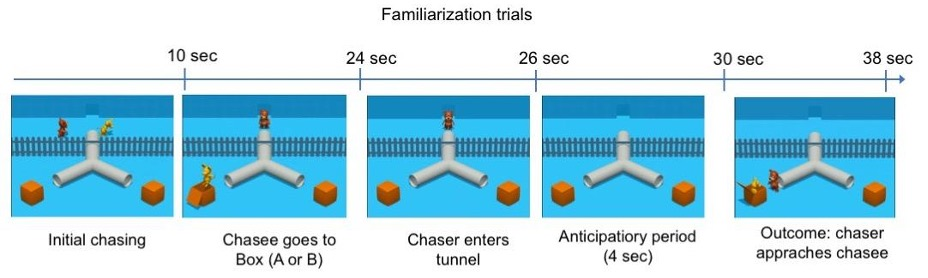
\includegraphics[width=6.8in]{/Users/mellischreiner/Documents/GitHub/mb2-analysis/paper/Figure1} 

}

\caption{Timeline of the familiarization trials.}\label{fig:fig1}
\end{figure}

\subsubsection{Familiarization Trials}\label{familiarization-trials}

All participants will view four familiarization trials (for an overview of key events see Figure 1). During familiarization trials, after a brief chasing introduction, the chasee enters an upside-down Y-shaped tunnel with a box at both of its exits. The chasee then leaves the tunnel through one of the exits and hides in the box on the corresponding side. Subsequently, the chaser enters the tunnel (to follow the chasee), and participants' AL to the tunnel exits is measured before the chaser exits on the side the chasee is hiding, as an index of their goal-based action anticipation. In these familiarization trials, if participants engage in spontaneous action anticipation, they should reliably anticipate that the chaser should emerge at the tunnel exit that leads to the box where the chasee is. After leaving the tunnel, the chaser approaches the box in which the chasee is hiding and knocks on it. Then, the chasee jumps out of the box and the two briefly interact.

\paragraph{Familiarization Phase Pilot Studies.}\label{familiarization-phase-pilot-studies.}

In a pilot study with 18- to 27-month-olds (\emph{n} = 65) and adults (\emph{n} = 42), seven labs used in-lab corneal reflection eye-tracking to collect data on gaze behavior in the familiarization phase. A key desideratum of our paradigm is that it should produce sufficient AL, as a low rate of AL in previous studies has led to high exclusion rates. The goals of the pilot study were to 1) estimate the level of correct goal-based action predictions in the familiarization phase, 2) determine the optimal number of familiarization trials, 3) check for issues with perceptual properties of stimuli (e.g., distracting visual saliencies), and 4) test the general procedure including preprocessing and analyzing raw gaze data from different eye-tracking systems. We found that the familiarization stimuli elicited a relatively high proportion of goal-directed action anticipations, but we were concerned about the effects of some minor properties of the stimulus (in particular, a small rectangular window in the tunnel tube that allowed participants to see the agents at one point on their path to the tunnel exits).
In a second pilot study with 18- to 27-month-olds (\emph{n} = 12, three participating labs), slight changes of stimulus features (the removal of the window in the tube; temporal changes of auditory anticipation cue) did not cause major changes in the AL rates.
Sixty-eight percent of toddlers' first looks in the first pilot, 69\% of toddlers' first looks in the second pilot, and 69\% of adults' first looks were toward the correct area of interest (AOI) during the anticipatory period. The average proportion of looking towards the correct AOI during the anticipatory period was 70.7\% (CI\textsubscript{95\%} = 67.6\% - 73.8\%) in toddlers in the first pilot, 70.5\% (CI\textsubscript{95\%} = 62.8\% - 78.2\%) in the second pilot for toddlers, and 75.3\% (CI\textsubscript{95\%} = 71.0\% - 79.5\%) in adults. In Bayesian analyses, we found strong evidence that toddlers and adults looked more towards the target than towards the distractor during the anticipation period. Based on conceptual and practical methodological considerations while also considering previous studies, we decided to include four trials in the final experiment. The pilot data results of the toddlers supported this decision insofar as we observed a looking bias towards the correct location already in trials 1-4, without additional benefit of trials 5-8.
Further, prototypical analysis pipelines were established for combining raw gaze data from different eye-trackers. In short, we developed a way to resample gaze data from different eye-trackers to be at a common Hz rate and to define proportionally correct AOIs for different screen dimensions with the goal to merge all raw data into one data set for inferential statistics. The established analysis procedure is described further in the Data Preprocessing section below.
In sum, we concluded that this paradigm sufficiently elicits goal-directed action predictions, an important prerequisite for drawing any conclusion on AL behavior in the test trials of this study. A detailed description of the two pilot studies can be found in the Supplemental Material.

\subsubsection{Test Trials}\label{test-trials}

All participants will see two test trials, one \emph{knowledge} and one \emph{ignorance} trial. However, in line with common practice in ToM studies, the main comparison concerns the first test trial between-participants to avoid potential carryover effects. In addition, in exploratory analyses, we plan to assess whether results remain the same if both trials are taken into account and whether gaze patterns differ between the two trials (see Exploratory Analyses). If the results remain largely unchanged across the two trials, it may suggest that future studies could increase power by including multiple test trials.
In test trials, the chasee first hides in one of the boxes, but shortly thereafter the chasee leaves this box and hides in the second box, at the other tunnel exit. Critically, the chaser either witnesses (\emph{knowledge} condition) or does not witness (\emph{ignorance} condition) from which tunnel exit the chasee exited and thus where the chasee is currently hiding (for an overview, see Figure 2). In the \emph{knowledge} trials, the chaser observes all movements of the chasee. The chaser leaves for a brief period of time after the chasee entered the tunnel, but it returns before the chasee exits the tunnel. Therefore, no events take place in the chaser's absence. In the \emph{ignorance} trials, the chaser sees the chasee enter the tunnel, but then leaves. Therefore, the chaser does not see the chasee entering either box and only returns once the chasee is already hidden in the final location. Finally, the chaser enters the tunnel but does not appear in either exit. Rather, the scene ``freezes'' for four seconds and participants' AL is measured. Thus, the \emph{knowledge} and \emph{ignorance} conditions are matched for the chaser leaving for a period of time, but they differ in whether they warrant the chaser's epistemic access to the location of the chasee. No outcome is shown in either test trials.
When designing the \emph{knowledge} and \emph{ignorance} condition, we aimed at keeping all events and their timings parallel, except the crucial manipulation. We show the same events in both conditions. Where possible, all events also have the same duration. In the case of the chaser's absence in the \emph{knowledge} condition, there were two main options, both with inevitable trade-offs. First, we could have increased the duration of the chaser's absence in the \emph{knowledge} condition to match the duration of the chaser's absence in both conditions. Yet, this would potentially disrupt the flow of events, such as keeping track of the chasee's actions and the general scene dynamics, since nothing would happen for a substantial amount of time. Second, the chaser can be absent for a shorter time in the \emph{knowledge} than in the \emph{ignorance} condition, in which case the flow of events -- the chasee's actions and the general scene dynamics -- remains natural. We chose the second option because we reasoned that the artificial break in the \emph{knowledge} condition could disrupt the participant's tracking of the chaser's epistemic state, thus being a confound that would be more detrimental than the difference in the duration of absence. Further, the current contrast has the advantage that the chasee's sequence and timing of actions are identical in both conditions, thus minimizing the difference between conditions. Finally, with the current design, the duration of the chaser's absence will be closely matched in the later planned false belief - true belief contrast, because in the future false belief condition, the chaser has to be absent for fewer events (because the chaser witnesses the first hiding events after the chasee reappeared at the other side of the tunnel).

\begin{figure}

{\centering 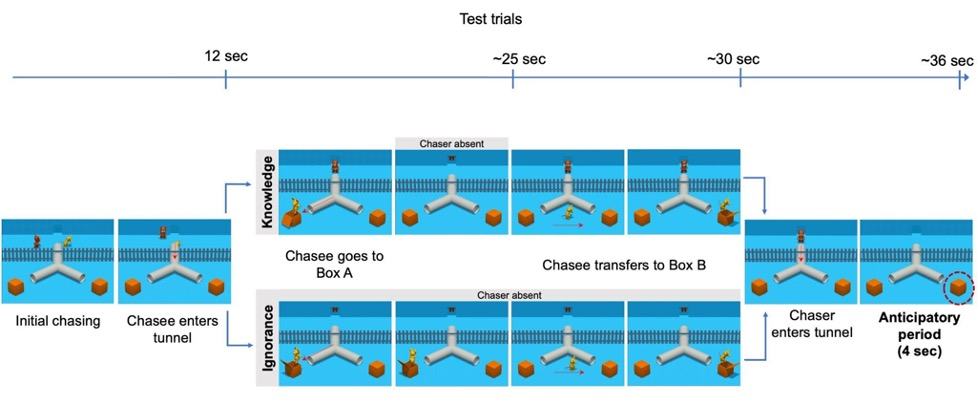
\includegraphics[width=6.5in]{/Users/mellischreiner/Documents/GitHub/mb2-analysis/paper/Figure2} 

}

\caption{Schematic overview of stimuli and conditions of the test trials. \newline{} \textit{Note}. After the familiarization phase, participants know about the agent’s goal (chaser wants to find chasee), perceptual access (chaser can see what happens on the other side of the fence), and situational constraints (boxes can be reached by walking through the forking tunnel). In the \textit{knowledge} condition, the chaser witnesses the chasee walking through the tunnel and jumping in and out of the first box. While the chasee is in the box, the chaser briefly leaves the scene through the door in the back and returns shortly after. Subsequently, the chaser watches the chasee jumping out of the box again and hiding in the second box. In the \textit{ignorance} condition, the chaser turns around and stands on the other side of the door in the back of the scene, thus unable to witness any of the chasee’s actions. The chaser then returns and enters the tunnel to look for the chasee. During the test phase (4 seconds still frame), AL towards the end of the tunnels is measured.}\label{fig:fig2}
\end{figure}

\subsubsection{Trial Randomization}\label{trial-randomization}

We will vary the starting location of the chasee (left or right half of the upper part of the scene) and the box the chasee ended up (left or right box) in both familiarization and test trials. The presentation of the familiarization trials will be counterbalanced in two pseudo-randomized orders. Each lab signs up for one or two sets of 16-trial-combinations, for each of their tested age groups.

\subsection{Lab Participation Details}\label{lab-participation-details}

\subsubsection{Time-Frame}\label{time-frame}

The contributing labs will start data collection as soon as they are able to once our Registered Report receives an in-principle acceptance. The study will be submitted for Stage 2 review within one year after in-principle acceptance (i.e., post-Stage 1 review). We anticipate that this time window gives the individual labs enough flexibility to contribute the committed sample sizes; however, if this timeline needs adjusting due to the Covid-19 pandemic this decision will be made prior to any data analysis.

\subsubsection{Participation Criterion}\label{participation-criterion}

The participating labs were recruited from the MB2 consortium. In July 2020, we asked via the MB2 listserv which labs plan to contribute how many participants for the respective age group (toddlers and/or adults). The Supplemental Material provides an overview of participating labs. Each lab made a commitment to collecting data from at least 16 participants (toddlers or adults), but we will not exclude any contributed data on the basis of the total sample size contributed by that lab. Labs will be allowed to test using either in-lab eye-tracking or online methods.

\subsubsection{Ethics}\label{ethics}

All labs will be responsible for obtaining ethics approval from their appropriate institutional review board. The labs will contribute de-identified data for central data analysis (i.e., eye-tracking raw data/coded gaze behavior, demographic information). Video recordings of the participants will be stored at each lab according to the approved local data handling protocol. If allowed by the local institutional review board, video recordings will be made available to other researchers via the video library Databrary (\url{https://nyu.databrary.org/}).

\subsubsection{Participants}\label{participants}

In a preliminary expression of interest, 26 labs signed up to contribute a minimal sample size of 16 toddlers and/or adults. Based on this information, we expect to recruit a total sample of 520 toddlers (ages 18-27 months) and 408 adults (ages 18-55 years). To avoid an unbalanced age distribution in the toddlers sample, labs will sign up for testing at least one of two age bins (bin 1: 18-22 months, bin 2: 23-27 months), and will be asked to ensure approximately equal distribution of participants' age in their collected sample if possible. They will be asked to try to ensure that the mean age of their sample lies in the middle of the range of the chosen bin and that participant ages are distributed across their whole bin. Both for adults and toddlers, basic demographic data will be collected on a voluntary basis with a brief questionnaire (see Supplemental Material for details). The requested demographic information that is not used in the registered confirmatory and/or exploratory analyses of this study will be collected for further potential follow-up analyses in spin-off projects within the MB framework.
After completing the task, adult participants will be asked to fill a funneled debriefing questionnaire. This questionnaire asks what the participant thinks the purpose of the experiment was, whether the participant had any particular goal or strategy while watching the videos, and whether the participant consciously tracked the chaser's epistemic state. Additionally, we collect details regarding each testing session (see Supplemental Material).

\begin{center}
\begin{ThreePartTable}

\footnotesize{

\begin{longtable}{lccccl}\noalign{\getlongtablewidth\global\LTcapwidth=\longtablewidth}
\caption{\label{tab:Lab and participant information}Lab and Participant information.}\\
\toprule
Lab & N collected & N included & Sex (N   Female) & Mean Age (years) & Method\\
\midrule
\endfirsthead
\caption*{\normalfont{Table \ref{tab:Lab and participant information} continued}}\\
\toprule
Lab & N collected & N included & Sex (N   Female) & Mean Age (years) & Method\\
\midrule
\endhead
CogConcordia & 21 & 16 & 11 & 22.12 & In-lab\\
CorbitLab & 16 & 15 & 14 & 19.87 & In-lab\\
DevlabAU & 20 & 20 & 15 & 25.15 & In-lab\\
MEyeLab & 53 & 53 & 39 & 24.47 & In-lab\\
MiniDundee & 15 & 13 & 10 & 30.23 & In-lab\\
PKUSu & 39 & 32 & 19 & 22.66 & In-lab\\
SkidLSDLab & 11 & 8 & 3 & 21.62 & In-lab\\
ToMcdlSalzburg & 33 & 31 & 22 & 27.23 & In-lab\\
UIUCinfantlab & 36 & 32 & 25 & 19.06 & In-lab\\
WSUMARCS & 18 & 13 & 8 & 29.85 & In-lab\\
affcogUTSC & 23 & 8 & 5 & 20.88 & web-based\\
babyLeidenEdu & 20 & 16 & 12 & 23.31 & In-lab\\
babylabAmsterdam & 17 & 16 & 13 & 24.00 & In-lab\\
babylabBrookes & 67 & 65 & 49 & 21.78 & In-lab\\
babylabINCC & 18 & 18 & 12 & 31.00 & In-lab\\
babylabMPIB & 16 & 16 & 11 & 27.44 & In-lab\\
babylabNijmegen & 19 & 15 & 13 & 22.13 & In-lab\\
babylabTrento & 16 & 16 & 9 & 21.69 & In-lab\\
babylabUmassb & 33 & 11 & 10 & 19.00 & In-lab\\
babyuniHeidelberg & 16 & 16 & 14 & 22.06 & In-lab\\
beinghumanWroclaw & 19 & 16 & 9 & 32.75 & web-based\\
careylabHarvard & 18 & 15 & 12 & 19.80 & In-lab\\
cclUNIRI & 32 & 32 & 17 & 30.53 & In-lab\\
childdevlabAshoka & 16 & 16 & 8 & 30.88 & In-lab\\
collabUIOWA & 16 & 16 & 10 & 19.19 & In-lab\\
gaugGöttingen & 30 & 28 & 18 & 31.71 & In-lab\\
jmuCDL & 32 & 32 & 22 & 18.81 & In-lab\\
kidsdevUniofNewcastle & 15 & 14 & 7 & 33.57 & In-lab\\
labUNAM & 20 & 11 & 8 & 22.45 & In-lab\\
lmuMunich & 31 & 30 & 23 & 22.53 & In-lab\\
mecdmpihcbs & 19 & 19 & 10 & 27.79 & In-lab\\
socialcogUmiami & 16 & 15 & 9 & 19.27 & In-lab\\
sociocognitivelab & 17 & 17 & 11 & 32.12 & In-lab\\
tauccd & 15 & 12 & 6 & 24.50 & In-lab\\
Total & 803 & 703 & 484 & 24.75 & \\
\bottomrule
\end{longtable}

}

\end{ThreePartTable}
\end{center}

\begin{center}
\begin{ThreePartTable}

\footnotesize{

\begin{longtable}{lccccc}\noalign{\getlongtablewidth\global\LTcapwidth=\longtablewidth}
\caption{\label{tab:Lab and participant information}Lab and Participant information.}\\
\toprule
Lab & N collected & N included & Sex (N   Female) & Mean Age (months) & Method\\
\midrule
\endfirsthead
\caption*{\normalfont{Table \ref{tab:Lab and participant information} continued}}\\
\toprule
Lab & N collected & N included & Sex (N   Female) & Mean Age (months) & Method\\
\midrule
\endhead
CogConcordia & 21 & 8 & 4 & 22.92 & web-based\\
CorbitLab & 11 & 10 & 5 & 22.77 & In-lab\\
DevlabAU & 18 & 17 & 8 & 19.00 & In-lab\\
PKUSu & 50 & 32 & 13 & 20.84 & In-lab\\
SkidLSDLab & 8 & 2 & 0 & 20.11 & In-lab\\
ToMcdlSalzburg & 17 & 12 & 6 & 22.20 & In-lab\\
UIUCinfantlab & 18 & 15 & 9 & 21.96 & In-lab\\
babyLeidenEdu & 18 & 12 & 8 & 22.59 & In-lab\\
babylabAmsterdam & 28 & 12 & 6 & 23.19 & In-lab\\
babylabBrookes & 17 & 12 & 7 & 22.15 & In-lab\\
babylabChicago & 17 & 13 & 4 & 20.10 & In-lab\\
babylabINCC & 16 & 9 & 6 & 23.40 & In-lab\\
babylabNijmegen & 19 & 10 & 3 & 23.52 & In-lab\\
babylabOxford & 25 & 19 & 8 & 23.42 & In-lab\\
babylabPrinceton & 17 & 11 & 7 & 22.15 & In-lab\\
babylabTrento & 18 & 17 & 10 & 22.72 & In-lab\\
babylabUmassb & 7 & 6 & 2 & 20.35 & In-lab\\
babylingOslo & 17 & 14 & 7 & 21.99 & In-lab\\
babyuniHeidelberg & 16 & 12 & 4 & 22.69 & In-lab\\
beinghumanWroclaw & 24 & 14 & 7 & 23.77 & web-based\\
careylabHarvard & 17 & 12 & 5 & 21.99 & In-lab\\
cecBYU & 16 & 14 & 4 & 22.39 & In-lab\\
childdevlabAshoka & 16 & 10 & 6 & 22.44 & In-lab\\
gaugGöttingen & 28 & 15 & 9 & 23.06 & In-lab\\
gertlabLancaster & 21 & 17 & 8 & 23.03 & In-lab\\
infantcogUBC & 26 & 19 & 8 & 24.39 & In-lab\\
irlConcordia & 19 & 12 & 5 & 22.47 & In-lab\\
kidsdevUniofNewcastle & 16 & 14 & 9 & 22.36 & In-lab\\
kokuHamburg & 19 & 14 & 7 & 25.99 & In-lab\\
labUNAM & 18 & 12 & 7 & 22.68 & In-lab\\
lmuMunich & 48 & 24 & 16 & 22.68 & In-lab\\
mecdmpihcbs & 25 & 12 & 8 & 23.58 & In-lab\\
mpievaCCP & 22 & 18 & 10 & 23.33 & In-lab\\
saxelab & 31 & 15 & 2 & 23.13 & web-based\\
socallabUCSD & 47 & 15 & 4 & 22.09 & web-based\\
tauccd & 15 & 12 & 8 & 22.99 & In-lab\\
unicph & 43 & 29 & 16 & 21.50 & In-lab\\
Total & 809 & 521 & 256 & 22.48 & \\
\bottomrule
\end{longtable}

}

\end{ThreePartTable}
\end{center}

Our final dataset consisted of 1224 participants, with an overall exclusion rate of 24.16\% (toddlers: 35.60\%, adults: 12.67\%).
Tables 1 A. and B. show the distribution of included participants across labs, eye-tracking methods, and ages.
A final sample of 521 toddlers (49.14\% female) that were tested in 37 labs (mean lab sample size = 14.08, \emph{SD} = 5.56, range: 2 - 32) was analyzed.
The average age of toddlers in the final sample was 22.49 months (\emph{SD}: 2.53, range: 18 - 27.01).
The final sample size of included adults was \emph{N} = 703 (68.85\% female), tested in 34 labs (mean lab sample size = 20.68, \emph{SD} = 12.14, range: 8 - 65).
Their mean age was 24.61 years (\emph{SD}: 7.36, range: 18 - 55).

\subsection{Apparatus and Procedure}\label{apparatus-and-procedure}

\subsubsection{Eye-tracking Methods}\label{eye-tracking-methods}

We expect that participating labs will use one of three types of eye-tracker brands to track the participant's gaze patterns: Tobii, EyeLink, or SMI. Thus, apparatus setup will slightly vary in individual labs (e.g., different sampling rates and distances at which the participants are seated in front of the monitor). Participating labs will report their eye-tracker specifications and study procedure alongside the collected data. To minimize variation between labs, all labs using the same type of eye-tracker will use the same presentation study file specific to that eye-tracker type. The Supplemental Material will provide an overview of employed eye-trackers, stimulus presentation softwares, sampling rates and screen dimensions.

\subsubsection{Online Gaze Recording}\label{online-gaze-recording}

To allow for the participation of labs that do not have access to an eye-tracker, or are not able to invite participants to their facilities due to current restrictions regarding the COVID-19 pandemic, labs can choose to collect data via online testing. Specifically, labs may choose to manually code gaze direction during stimulus presentation on a frame-by-frame basis from video recordings of a camera facing the participant (e.g., a webcam). Labs that choose to collect data virtually will utilize the platform of their choice (e.g., LookIt, YouTube, Zoom, Labvanced, etc.). Further, labs may also choose to use webcam eye-tracking with tools like WebGazer.js (Papoutsaki et al., 2016). In our analyses, we control for and quantify potential sources of variability due to these different methods.

\subsubsection{Testing Procedure}\label{testing-procedure}

Toddlers will be seated either on their caregiver's lap or in a highchair. The distance from the monitor will depend on the data collection method. Caregivers will be asked to refrain from interacting with their child and close their eyes during stimulus presentation or wear a set of opaque sunglasses. Adult participants will be seated on a chair within the respective appropriate distance from the monitor. Once the participant is seated, the experimenter will initiate the eye-tracker-specific calibration procedure. Additionally, we will present another calibration stimulus before and after the presentation of the task. This allows for evaluating the accuracy of the calibration procedure across labs (cf., Frank, Vul, \& Saxe, 2012).

\subsection{General Lab Practices}\label{general-lab-practices}

To ensure standardization of procedure, materials for testing practices and instructions will be prepared and distributed to the participating labs. Each lab will be responsible for maintaining these practices and report all relevant details on testing sessions (for details see the Supplemental Material).

\subsubsection{Videos of Participants}\label{videos-of-participants}

As with all MB projects, we strongly encourage labs to record video data of their own lab procedures and each testing session, provided that this is in line with regulations of the respective institutional ethics review board and the given informed consent. Participating labs that cannot contribute participant videos will be asked to provide a video walk-through of their experimental set-up and procedure instead. If no institutional ethics review board restrictions occur, labs are encouraged to share video recordings of the test sessions via DataBrary.

\subsection{Design Analysis}\label{design-analysis}

Here we provide a simulation of the predicted findings because a traditional frequentist power analysis is not applicable for our project for two reasons. First, we use Bayesian methods to quantify the strength of our evidence for or against our hypotheses, rather than assessing the probability of rejecting the null hypothesis. In particular, we compute a Bayes factor (BF; a likelihood ratio comparing two competing hypotheses), which allows us to compare models. Second, because of the many-labs nature of the study, the sample size will not be determined by power analysis, but by the amount of data that participating labs are able to contribute within the pre-established timeframe. Even if the effect size is much smaller than what we anticipate (e.g., less than Cohen's \emph{d} = 0.20), the results would be informative as our study is expected to be dramatically larger than any previous study in this area. If, due to unforeseen reasons, the participating labs will not be able to collect a minimum number of 300 participants per age group within the proposed time period, we plan to extend the time for data collection until this minimum number is reached. Or in contrast, if the effect size is large (e.g., more than Cohen's \emph{d} = 0.80), the resulting increased precision of our model will allow us to test a number of other theoretically and methodologically important hypotheses (see Results section).
Although we did not determine our sample size based on power analysis, here we provide a simulation-based design analysis to demonstrate the range of BFs we might expect to see, given a plausible range of effect sizes and parameters. We focus this analysis on our key analysis of the test trials (as specified below), namely the difference in AL on the first test trial that participants saw. We describe below the simulation for the child sample, but based on our specifications, we expect that a design analysis for adult data would produce similar results.
We first ran a simulation for the first look analysis. In each iteration of our simulation, we used a set of parameters to simulate an experiment, using a first look (described below) as the key measure. For the key effect size parameter for condition (\emph{knowledge} vs.~\emph{ignorance}), we sampled a range of effect sizes in logit space spanning from small to large effects (Cohen's \emph{d} = 0.20 - 0.80; log odds from 0.36 - 1.45). For each experiment, the betas for age and the age x condition interaction were sampled uniformly between -0.20 and 0.20. The age of each participant was sampled uniformly between 18 and 27 months and then centered. The intercept was sampled from a normal distribution (1, 0.25), corresponding to an average looking proportion of 0.73. Lab intercepts and the lab slope by condition were set to 0.1, and other lab random effects were set to 0 as we do not expect them to be meaningfully non-zero. These values were chosen based on pilot data (average looking proportion), but also to have a large range of possible outcomes (lab intercept, age and age x condition interaction). We are confident that the results would be robust to different choices. We then used these simulated data to simulate an experiment with 22 labs and 440 toddlers and computed the resulting BFs, as specified in the analysis plan below. We adopted all of the priors specified in the results section below\footnote{After the design analysis, additional labs expressed their interest in contributing data, which is why the anticipated sample sizes and the numbers this design analysis is based on differ. Given the uncertainty in determining the final sample size in this project, we kept the design analysis as is to have a more conservative estimate of the study's power.}. We ran 349 simulations and, in 72\% of them, the BF showed strong evidence in favor of the full model (BF \textgreater{} 10); in 6\% the BF showed substantial evidence (10 \textgreater{} BF \textgreater{} 3); it was inconclusive 14\% of the time (1/10 \textgreater{} BF \textgreater{} 3), and in 8\% of cases the null model was substantially favored (see Supplement). The BF was not \textless{} 1/10 in any of the simulations.. Thus, under the parameters chosen here for our simulations, it is likely that the planned experiment is of sufficient size to detect the expected effect.
We also ran a design analysis for the proportional looking analysis. We used the same experimental parameters (number of labs, participants, ages, etc.). For generating simulated data, we drew the condition effect from a uniform distribution between .05 and .20 (in proportion space). The age and age:condition effects were drawn from uniform distributions between -.05 and .05. Sigma, the overall noise in the experiment, was drawn from a uniform distribution between .05 and .1. The intercept was drawn from a normal distribution with mean .65 and a standard deviation of .05. The by-lab standard deviation for the intercept and condition slope was set to .01. Priors were as described in the main text. We ran 119 simulations, and in all 119 we obtained a BF greater than 10, suggesting that, under our assumptions, the study is well-powered.

\subsection{Data Preprocessing}\label{data-preprocessing}

\subsubsection{Eye-tracking}\label{eye-tracking}

Raw gaze position data (x- and y-coordinates) will be extracted in the time window starting from the first frame at which the chaser enters the tunnel until the last frame before it exits the tunnel in the last familiarisation trial and in the test trial. For data collected from labs using a binocular eye-tracker, gaze positions of the left and the right eye will be averaged.
We will use the peekds R package (\url{https://github.com/peekbank/peekbankr}) to convert eye-tracking data from disparate trackers into a common format. Because not all eye-trackers record data with the same frequency or regularity, we will resample all data to be at a common rate of 40 Hz (samples per second).
We will exclude individual trials if more than 50\% of the gaze data is missing (defined as off-screen or unavailable point of gaze during the whole trial, not just the anticipatory period). Applying this criterion would have caused us to exclude 4\% of the trials in our pilot data, which inspection of our pilot data suggested was an appropriate trade-off between not excluding too much usable data and not analyzing trials which were uninformative.
For each monitor size, we will determine the specific AOIs and compute whether the specific x- and y-position for each participant, trial, and time point fall within their screen resolution-specific AOIs. Our goal is to determine whether participants are anticipating the emergence of the chaser from one of the two tunnel exits. Thus, we defined AOIs on the stimulus by creating a rectangular region around the tunnel exit that is D units from the top, bottom, left, and right of the boundary of the tunnel exit, where D is the diameter of the tunnel exits. We then expanded the sides of the AOI rectangles by 25\% in all directions to account for tracker calibration error. Our rationale was that, if we made the AOI too small, we might fail to capture anticipations by participants with poor calibrations. In contrast, if we made the regions too large, we might capture some fixations by participants looking at the box where the chasee actually is. On the other hand, these chasee looks would not be expected to vary between conditions and so would only affect our baseline level of looking. Thus, the chosen AOIs aim at maximizing our ability to capture between-condition differences. For an illustration of the tunnel exit AOIs see Figure 3. We are not analyzing looks to the boxes, since they can less unambiguously be interpreted as epistemic state-based action predictions and because we observed few anticipatory looks to the boxes in the pilot studies. For more detailed information about the AOI definition process see the description of the pilot study results in the Supplemental Material.

\begin{figure}

{\centering 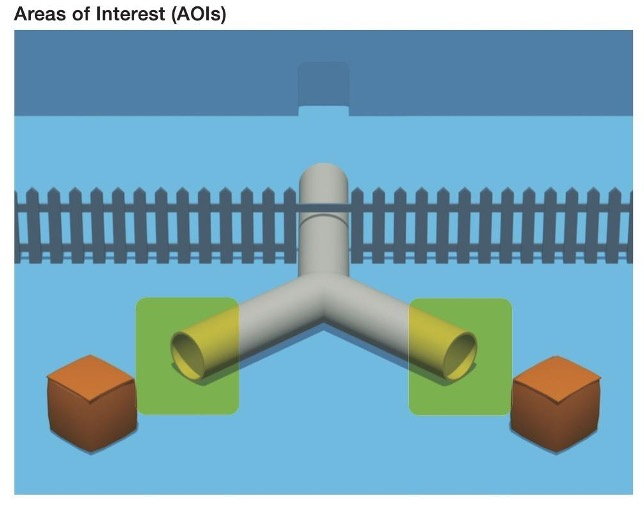
\includegraphics[width=4in]{/Users/mellischreiner/Documents/GitHub/mb2-analysis/paper/Figure4} 

}

\caption{Illustration of Areas of Interest (AOIs) for gaze data analysis during the anticipatory period. \newline{} \textit{Note}. The light green rectangles show the dimensions of the AOIs used for the analysis of AL during the test period.}\label{fig:fig3}
\end{figure}

\subsubsection{Manual Coding}\label{manual-coding}

For data gathered without an eye-tracker (e.g., videos of participants gathered from online administration), precise estimation of looks to specific AOIs will not be possible. Instead, videos will be coded for whether participants are looking to the left or the right side of the screen (or ``other/off screen''). In our main analysis, during the critical anticipatory window, we will treat these looks identically to looks to the corresponding AOI. See exploratory analyses for analysis of data collected online.

\subsubsection{Temporal Region of Interest}\label{temporal-region-of-interest}

For familiarization trials, we define the start of the anticipatory period (total length = 4000 ms) as starting 120 ms after the first frame after which the chaser has completely entered the tunnel and lasting until 120 ms after the first frame at which the chaser is visible again {[}we chose 120 ms as a conservative value for cutting off reactive saccades; cf., Yang, Bucci, and Kapoula (2002){]}. For test trials, we define the start of the anticipatory period in the same way, with a total duration of 4000 ms.

\subsubsection{Dependent Variables}\label{dependent-variables}

We define two primary dependent variables:
1. First look. First saccades will be determined as the first change in gaze occurring within the anticipatory time window that is directed towards one of the AOIs. The first look is then the binary variable denoting the target of this first saccade (i.e., either the correct or incorrect AOI) and is defined as the first AOI where participants fixated at for at least 150 ms, as in Rayner, Smith, Malcolm, and Henderson (2009). The rationale for this definition was that, if participants are looking at a location within the tunnel exit AOIs before the anticipation period, they might have been looking there for other reasons than action prediction. We therefore count only looks that start within the anticipation period because they more unambiguously reflect action predictions. This further prevents us from running into a situation where we would include a lot of fixations on regions other than the tunnel exit AOIs because participants are looking somewhere else before the anticipation period begins.
2. Proportion DLS {[}also referred to as total relative looking time; Senju et al. (2009){]}. We compute the proportion looking (p) to the correct AOI during the full 4000 ms anticipatory window (correct looking time / (correct looking time + incorrect looking time)), excluding looks outside of either AOI.

\section{Results}\label{results}

\subsection{Confirmatory Analyses}\label{confirmatory-analyses}

\subsubsection{Approach.}\label{approach.}

As discussed in the Methods section, we adopted a Bayesian analysis strategy so as to maximize our ability to make inferences about the presence or absence of a condition effect (i.e., our key effect of interest). In particular, we fit Bayesian mixed effects regressions using the package brms in R (Bürkner, 2017). This framework allows us to estimate key effects of interest while controlling for variability across grouping units (in our case, labs).
To facilitate interpretation of individual coefficients, we report means and credible intervals. For key inferences in our confirmatory analysis, we use the bridge sampling approach (Gronau et al., 2017) to compute BFs comparing different models. As the ratio of the likelihood of the observed data under two different models, BFs allow us to quantify the evidence that our data provide with respect to key comparisons. For example, by comparing models with and without condition effects, we can quantify the strength of the evidence for or against such effects.
Bayesian model comparisons require the specification of proper priors on the coefficients of individual models. Here, for our first look analysis, we use a set of weakly informative priors that capture the expectation that the effects that we observe (of condition and, in some cases, trial order) are modest. For coefficients, we choose a normal distribution with mean of 0 and \emph{SD} of 2. Based on our pilot testing and the results of MB1, we assume that lab and participant-level variation will be relatively small, and so for the standard deviation of random effects (i.e., variation in effects across labs and, in the case of the familiarization trials, participants) we set a Normal prior with mean of 0 and \emph{SD} of 0.1. We set an LKJ(2) prior on the correlation matrix in the random effect structure, a prior that is commonly used in Bayesian analyses of this type (Bürkner, 2017). Because the BF is sensitive to the choice of prior, we also ran a secondary analysis with a less informative prior: fixed effect coefficients chosen from a normal distribution with mean 0 and \emph{SD} of 3, and random effect standard deviations drawn from a normal prior with a mean of 0 and \emph{SD} of 0.5 (see Supplement S3). With respect to the specification of random effects, we followed the approach advocated by Barr (2013), that is, specifying the maximal random effect structure justified by our design. Since we are interested in lab-level variation, we will fit random effect coefficients for fixed effects of interest within labs (e.g., condition within lab). Further, where there were participant-level repeated measure data (e.g., familiarization trials), we fitted random effects of participants.
For the proportional looking score analysis, we used a uniform prior on the intercept between -0.5 and 0.5 (corresponding to proportional looking scores between 0 and 1: the full possible range). For the priors on the fixed effect coefficients, we used a normal prior with a mean of 0 and an \emph{SD} of 0.1. Because these regressions are in proportion space, 0.10 corresponds to a change in proportion of 10\%. For the random effect priors, we used a normal distribution with mean 0 and standard deviation .05. The LKJ prior was specified as above.
All preregistered confirmatory models converged, with no divergent transitions, all Rhat values \textless{} 1.1, and an effective sample size greater than 20\% of the total sample size.

\begin{figure}

{\centering 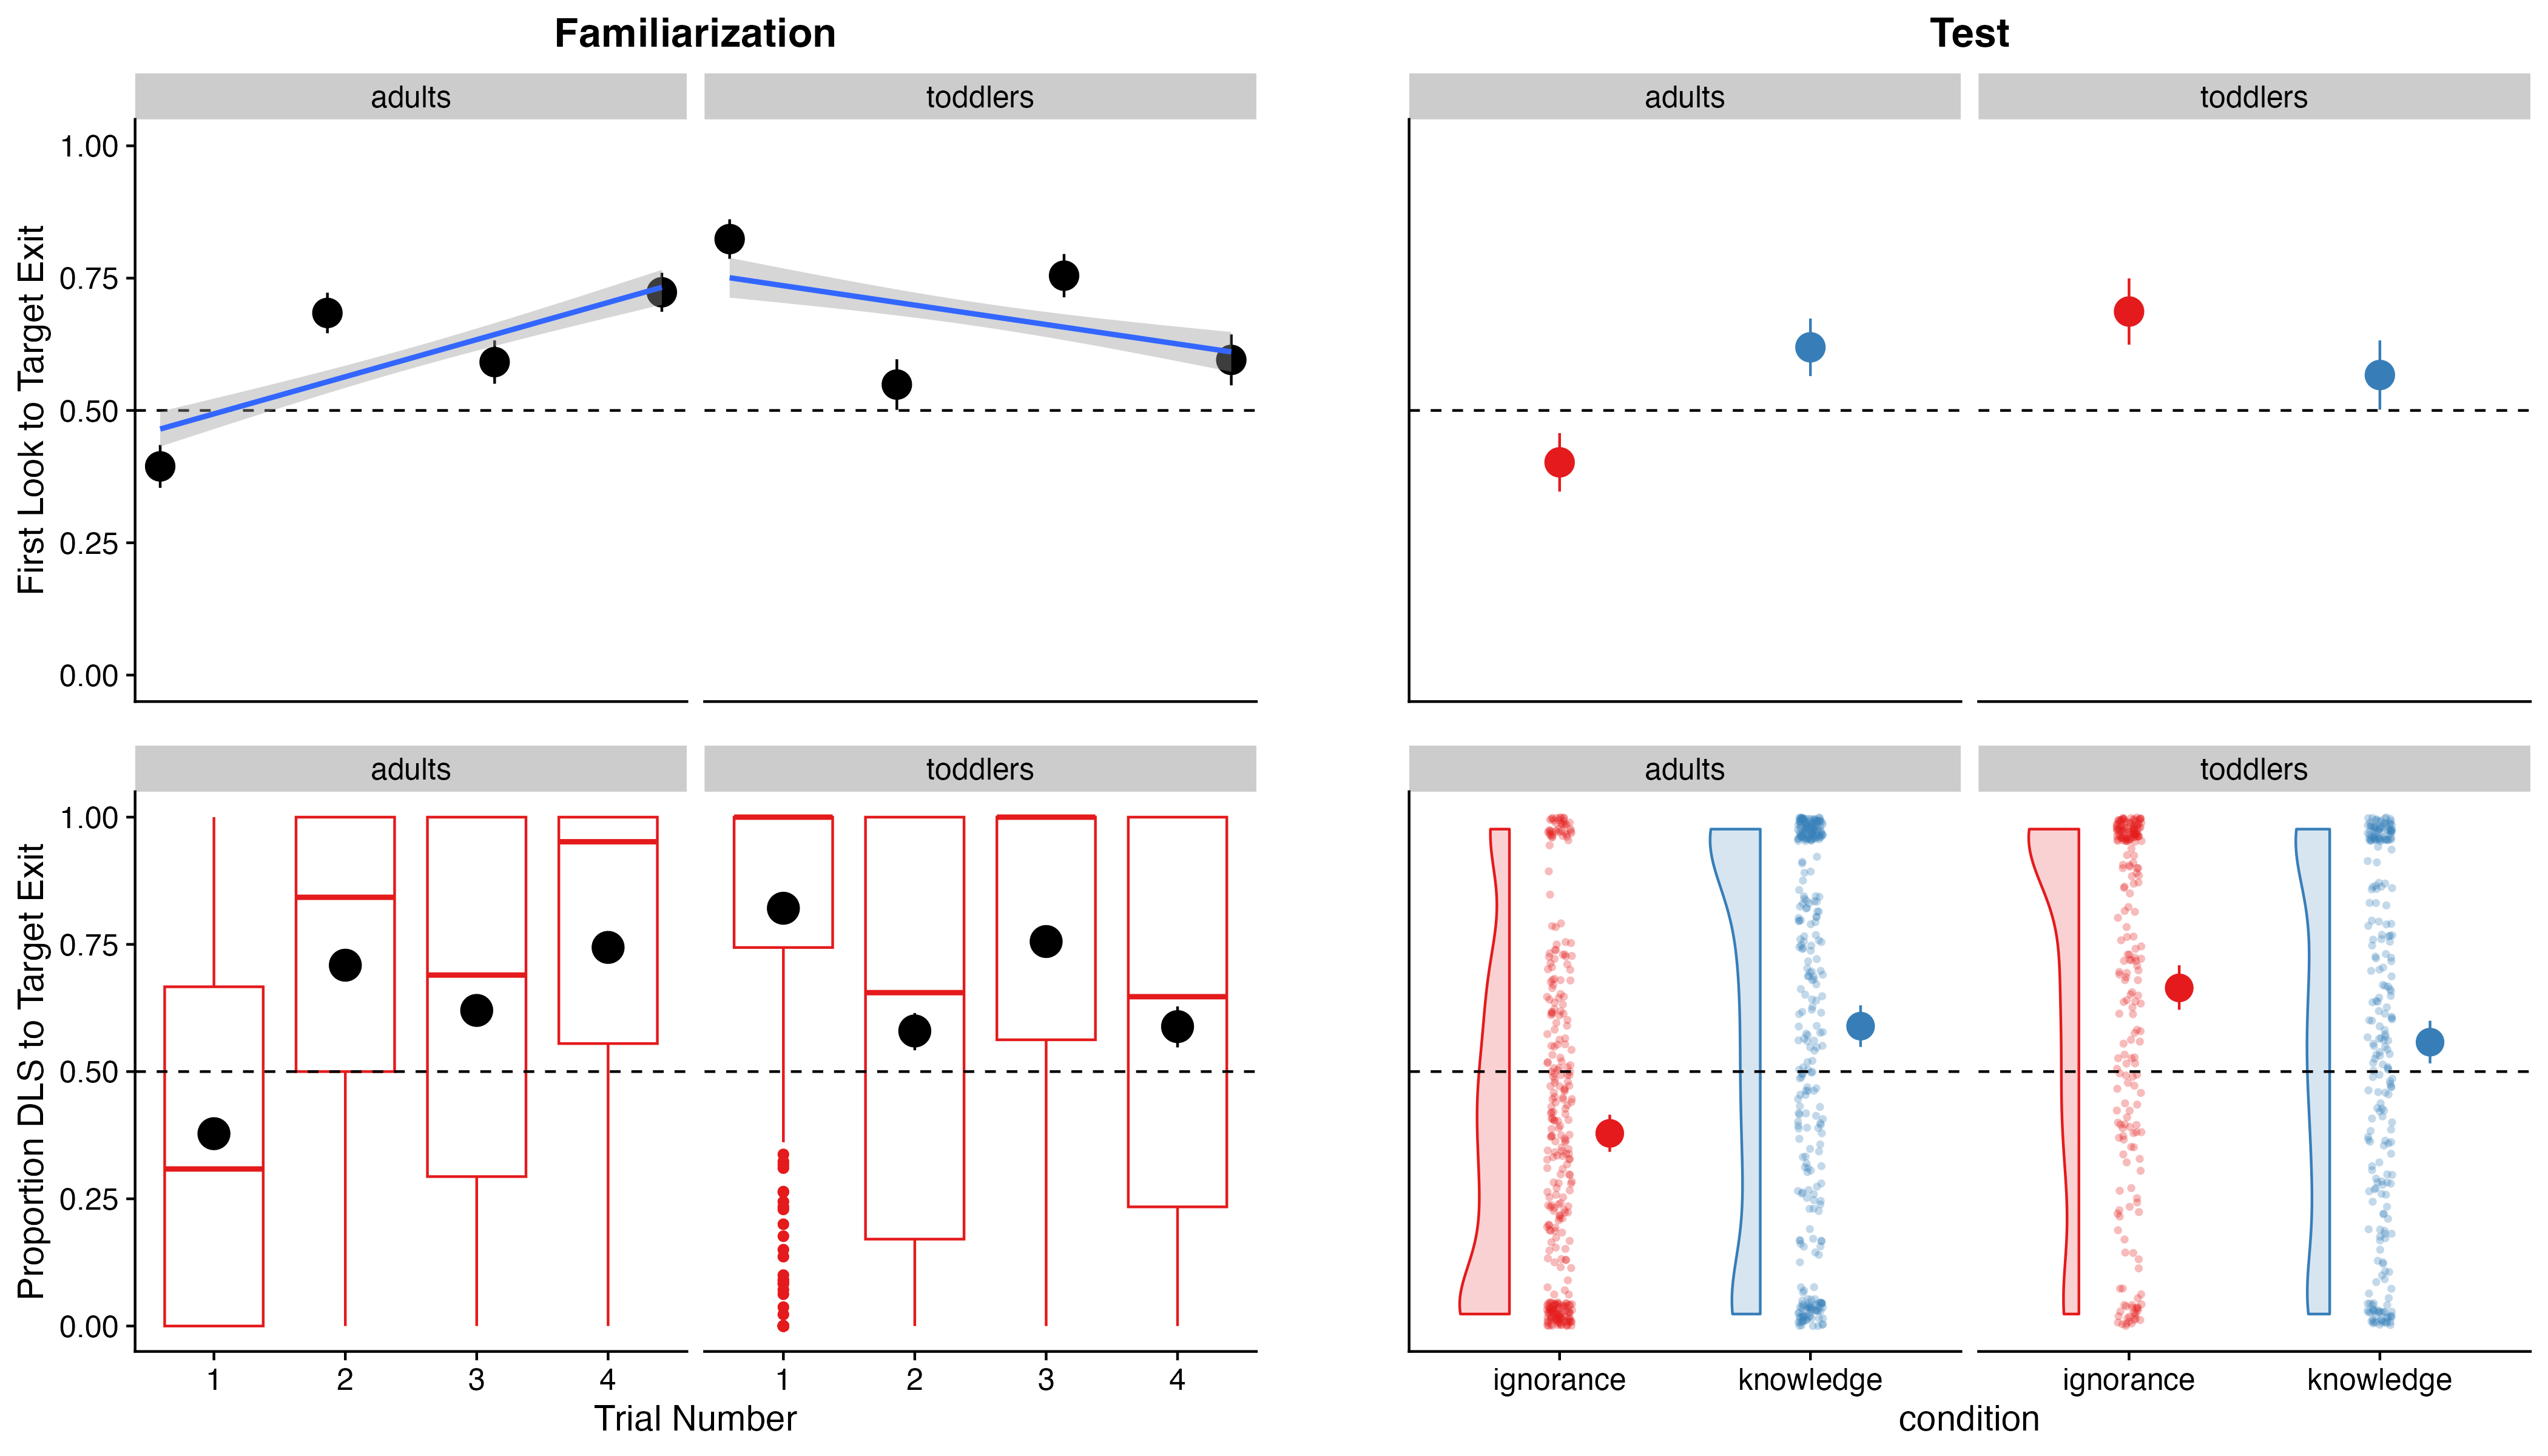
\includegraphics[width=6.8in]{/Users/mellischreiner/Documents/GitHub/mb2-analysis/paper/Figure5} 

}

\caption{Proportional target looking and proportion of first looks for toddlers and adults during familiarization and test.}\label{fig:fig4}
\end{figure}

\begin{center}
\begin{ThreePartTable}

\footnotesize{

\begin{longtable}{llrrrrr}\noalign{\getlongtablewidth\global\LTcapwidth=\longtablewidth}
\caption{\label{tab:Results table of Bayesian regression models}Results of the Bayesian mixed effects models for the familiarization trials.}\\
\toprule
model & \multicolumn{1}{c}{term} & \multicolumn{1}{c}{estimate} & \multicolumn{1}{c}{est\_error} & \multicolumn{1}{c}{lower\_ci} & \multicolumn{1}{c}{upper\_ci} & \multicolumn{1}{c}{rhat}\\
\midrule
\endfirsthead
\caption*{\normalfont{Table \ref{tab:Results table of Bayesian regression models} continued}}\\
\toprule
model & \multicolumn{1}{c}{term} & \multicolumn{1}{c}{estimate} & \multicolumn{1}{c}{est\_error} & \multicolumn{1}{c}{lower\_ci} & \multicolumn{1}{c}{upper\_ci} & \multicolumn{1}{c}{rhat}\\
\midrule
\endhead
fl toddlers & Intercept & 0.44 & 0.09 & 0.27 & 0.61 & 1.00\\
 & Trial Number & -0.22 & 0.05 & -0.32 & -0.12 & 1.00\\
fl adults & Intercept & 1.03 & 0.09 & 0.86 & 1.20 & 1.00\\
 & Trial Number & 0.38 & 0.04 & 0.30 & 0.47 & 1.00\\
aoi toddlers & Intercept & 0.12 & 0.02 & 0.09 & 0.15 & 1.00\\
 & Trial Number & -0.05 & 0.01 & -0.06 & -0.03 & 1.00\\
aoi adults & Intercept & 0.26 & 0.02 & 0.23 & 0.29 & 1.00\\
 & Trial Number & 0.10 & 0.01 & 0.09 & 0.11 & 1.00\\
\bottomrule
\end{longtable}

}

\end{ThreePartTable}
\end{center}

\begin{center}
\begin{ThreePartTable}

\footnotesize{

\begin{longtable}{llrrrrr}\noalign{\getlongtablewidth\global\LTcapwidth=\longtablewidth}
\caption{\label{tab:Results table of Bayesian regression models}Results of the Bayesian mixed effects models for the test trials.}\\
\toprule
model & \multicolumn{1}{c}{term} & \multicolumn{1}{c}{estimate} & \multicolumn{1}{c}{est\_error} & \multicolumn{1}{c}{lower\_ci} & \multicolumn{1}{c}{upper\_ci} & \multicolumn{1}{c}{rhat}\\
\midrule
\endfirsthead
\caption*{\normalfont{Table \ref{tab:Results table of Bayesian regression models} continued}}\\
\toprule
model & \multicolumn{1}{c}{term} & \multicolumn{1}{c}{estimate} & \multicolumn{1}{c}{est\_error} & \multicolumn{1}{c}{lower\_ci} & \multicolumn{1}{c}{upper\_ci} & \multicolumn{1}{c}{rhat}\\
\midrule
\endhead
fl toddlers & Intercept & 0.53 & 0.11 & 0.32 & 0.74 & 1.00\\
 & Condition & 0.53 & 0.21 & 0.13 & 0.93 & 1.00\\
 & Age & 0.06 & 0.05 & -0.03 & 0.15 & 1.00\\
 & Condition:Age & -0.13 & 0.09 & -0.30 & 0.04 & 1.00\\
fl adults & Intercept & 0.05 & 0.09 & -0.12 & 0.22 & 1.00\\
 & Condition & -0.89 & 0.17 & -1.22 & -0.56 & 1.00\\
aoi toddlers & Intercept & 0.61 & 0.02 & 0.58 & 0.65 & 1.00\\
 & Condition & 0.10 & 0.03 & 0.03 & 0.17 & 1.00\\
 & Age & 0.01 & 0.01 & -0.01 & 0.02 & 1.00\\
 & Condition:Age & -0.01 & 0.02 & -0.04 & 0.02 & 1.00\\
aoi adults & Intercept & 0.48 & 0.02 & 0.45 & 0.51 & 1.00\\
 & Condition & -0.20 & 0.03 & -0.26 & -0.15 & 1.00\\
\bottomrule
\end{longtable}

}

\end{ThreePartTable}
\end{center}

\subsubsection{Familiarization Trials.}\label{familiarization-trials.}

Figure 4 shows the proportion of first looks and the proportion of target looking (non-logit transformed) for toddlers and adults plotted across familiarization trials and test trials. Our first set of analyses examined data from the four familiarization trials and asked whether participants anticipated the chaser's reappearance at one of the tunnel exits. In our first analysis, we were interested in whether participants engaged in AL during the familiarization trials. To quantify the level of familiarization, we fitted Bayesian mixed effect models predicting target looks based on trial number (1-4) with random effects for lab and participants and random slopes for trial number for each.
In R formula notation (which we adopt here because of its relative concision compared with standard mathematical notation), our base model was as follows:
\(measure \sim 1 + trial\_number +  (trial\_number | lab) + (trial\_number | participant).\)
We fitted a total of four instances of this model, one for each age group (toddlers vs.~adults) and dependent measure (proportion looking score vs.~first look). First look models were fitted using Bernoulli family with a logit link function. The proportion looking score models were Gaussian.
Our key question of interest was whether overall anticipation was higher than chance levels on the familiarization trial immediately before the test trials, in service of evaluating the evidence that participants were attentive and making predictive looks immediately prior to test. To evaluate this question across the four models, we coded trial number so that the last trial before the test trials (trial 4) was set to the intercept, allowing the model intercept to encode an estimate of the proportion of correct anticipation immediately before test. We then fitted a simpler model for comparison
\(measure \sim 0 + trial\_number +  (trial\_number | lab) + (trial\_number | participant),\)
which included no intercept term. We then computed the BF comparing this model to the full model. This BF quantified the evidence for an anticipation effect for each group and measure.

\paragraph{Proportion of first looks}\label{proportion-of-first-looks}

\subparagraph{Toddlers}\label{toddlers}

Investigating proportion of first looks to the target location for toddlers, we again used a Bayesian mixed effects model to predict whether toddlers' first look was to the target exit based on trial number (1-4), with random effects for lab and participants and random slopes for trial number for each.
The Bayes factor comparing the full model to the simpler model was estimated to be BF \textgreater{} 1000, favoring the full model over the null model. This confirmed that toddlers showed above-chance looking to the target location during the anticipatory window of the last familiarization trial.
The model also provided support for an effect of trial number on proportion of first looks, with the negative coefficient indicating a decrease in target looks across the familiarization trials.

\subparagraph{Adults}\label{adults}

Comparing the Bayesian mixed effects model of adults predicting proportion of first looks based on trial number (1-4), with random effects for lab and participants and random slopes for trial number for each with the simpler model without an intercept, we computed a Bayes factor of BF \textgreater{} 1000, strongly favoring the full model over the null model. Again, this suggested that also adults' anticipation was higher than chance levels on the last familiarization trial.
In addition, there was support for an effect of trial number on proportion of first looks, with the positive coefficient indicating an increase in proportion of first target looks across the familiarization trials.

\paragraph{Proportion of target looking}\label{proportion-of-target-looking}

\subparagraph{Toddlers}\label{toddlers-1}

We used a Bayesian mixed effects models to predict proportional target looking based on trial number (1-4) for toddlers, with random effects for lab and participants and random slopes for trial number for each. The Bayes factor comparing this model to the simpler null model without the intercept was estimated to be BF \textgreater{} 1000, strongly favoring the full model over the null model. See also Table 3 for regression coefficients for the full model. These results suggest a significant effect of trial number on PTL, with the negative coefficient indicating a decrease in PTL across the familiarization trials.

\subparagraph{Adults}\label{adults-1}

Next, we used a Bayesian mixed effects model to predict PTL based on trial number (1-4) for adults, again with random effects for lab and participants and random slopes for trial number for each. The Bayes factor for the full model against the null model was BF \textgreater{} 1000, suggesting strong evidence for the full model. These results suggest a significant effect of trial number on PTL, with the positive coefficient indicating an increase in target looks across the familiarization trials.

\subsubsection{Test Trials.}\label{test-trials.}

We focused our confirmatory analysis on the first test trial (see Exploratory Analysis section for an analysis of both trials). Our primary question of interest was whether AL differs between conditions (knowledge vs.~ignorance, coded as -.5/.5) and by age (in months, centered). For child participants, we fitted models with the specification:
\(measure \sim 1 + condition + age + condition:age + (1 + condition + age + condition:age | lab).\)
For adult participants, we fitted models with the specification
\(measure \sim 1 + condition + (1 + condition | lab).\)
Again, we fitted models with a logistic link for first look analyses and with a standard linear link for DLS.
In each case, our key BF was a comparison of this model with a simpler ``null'' model that did not include the fixed effect of condition but still included other terms. We took a BF \textgreater{} 3 in favor of a particular model as substantial evidence and a BF \textgreater{} 10 in favor of strong evidence. A BF \textless{} 1/3 was taken as substantial evidence in favor of the simpler model, and a BF \textless{} 1/10 as strong evidence in favor of the simpler model.
For the model of data from toddlers, we additionally were interested in whether the model showed changes in AL with age. We assessed evidence for this by computing BFs related to the comparison with a model that did not include an interaction between age and condition as fixed effects
\[measure \sim 1 + condition + age + (1 + condition + age + condition:age | lab).\]
These BFs captured the evidence for age-related changes in the difference in action anticipation between the two conditions.
It is important to note that in the case of a null effect, there are two main explanations: (1) toddlers and adults in our study do not distinguish between knowledgeable and ignorant agents when predicting their actions. (2) The method used is not appropriate to reveal knowledge/ignorance understanding. By using Bayesian analyses, we are able to better evaluate the first of these two possibilities: The BF provides a measure of our statistical confidence in the null hypothesis, i.e., no difference between experimental conditions, given the data in ways that standard null hypothesis significance testing does not. In other words, instead of merely concluding that we did not find a difference between conditions, we would be able to find no/anecdotal/moderate/strong/very strong/extreme evidence for the null hypothesis that our participants did not distinguish between knowledgeable and ignorant agents when predicting their actions (Schönbrodt \& Wagenmakers, 2018). We therefore consider this analysis an important addition to our overall analysis strategy. Yet, even our Bayesian analyses are not able to rule out the second possibility that participants may well show such knowledge/ignorance understanding with different methods, or that this ability may not be measurable with any methods available at the current time. Addressing this alternative explanation warrants follow up experiments.

\paragraph{Proportion of first looks}\label{proportion-of-first-looks-1}

\subparagraph{Toddlers}\label{toddlers-2}

Investigating proportion of first looks for toddlers, we again used a Bayesian mixed effects model to predict target looks based on condition, with random effects for lab. The Bayes factor comparing the full model to the simpler model was estimated to be BF = 2.4, providing only anecdotal evidence in favor of the full model over the null model.

Again, we examined whether age influenced the difference in action anticipation between knowledge and ignorance trials. To do this, we compared the full model, which included an interaction between age and condition, with a simpler model without this interaction. The computed Bayes factor, BF \textless{} 0.1, strongly supports the simpler model, suggesting that the interaction term does not substantially improve the model's fit. This implies that age does not appear to significantly affect the difference in action anticipation between the two trial types.

\subparagraph{Adults}\label{adults-2}

We compared a Bayesian mixed-effects model predicting the proportion of first looks based on condition, including random effects for lab to a simpler model without the main effect of condition. The analysis yielded a Bayes factor of BF \textgreater{} 1000, providing strong evidence in favor of the full model over the null model. Results indicated that first looks to the target were significantly more frequent in the knowledge condition compared to the ignorance condition.

\paragraph{Proportion of target looking}\label{proportion-of-target-looking-1}

\begin{figure}

{\centering 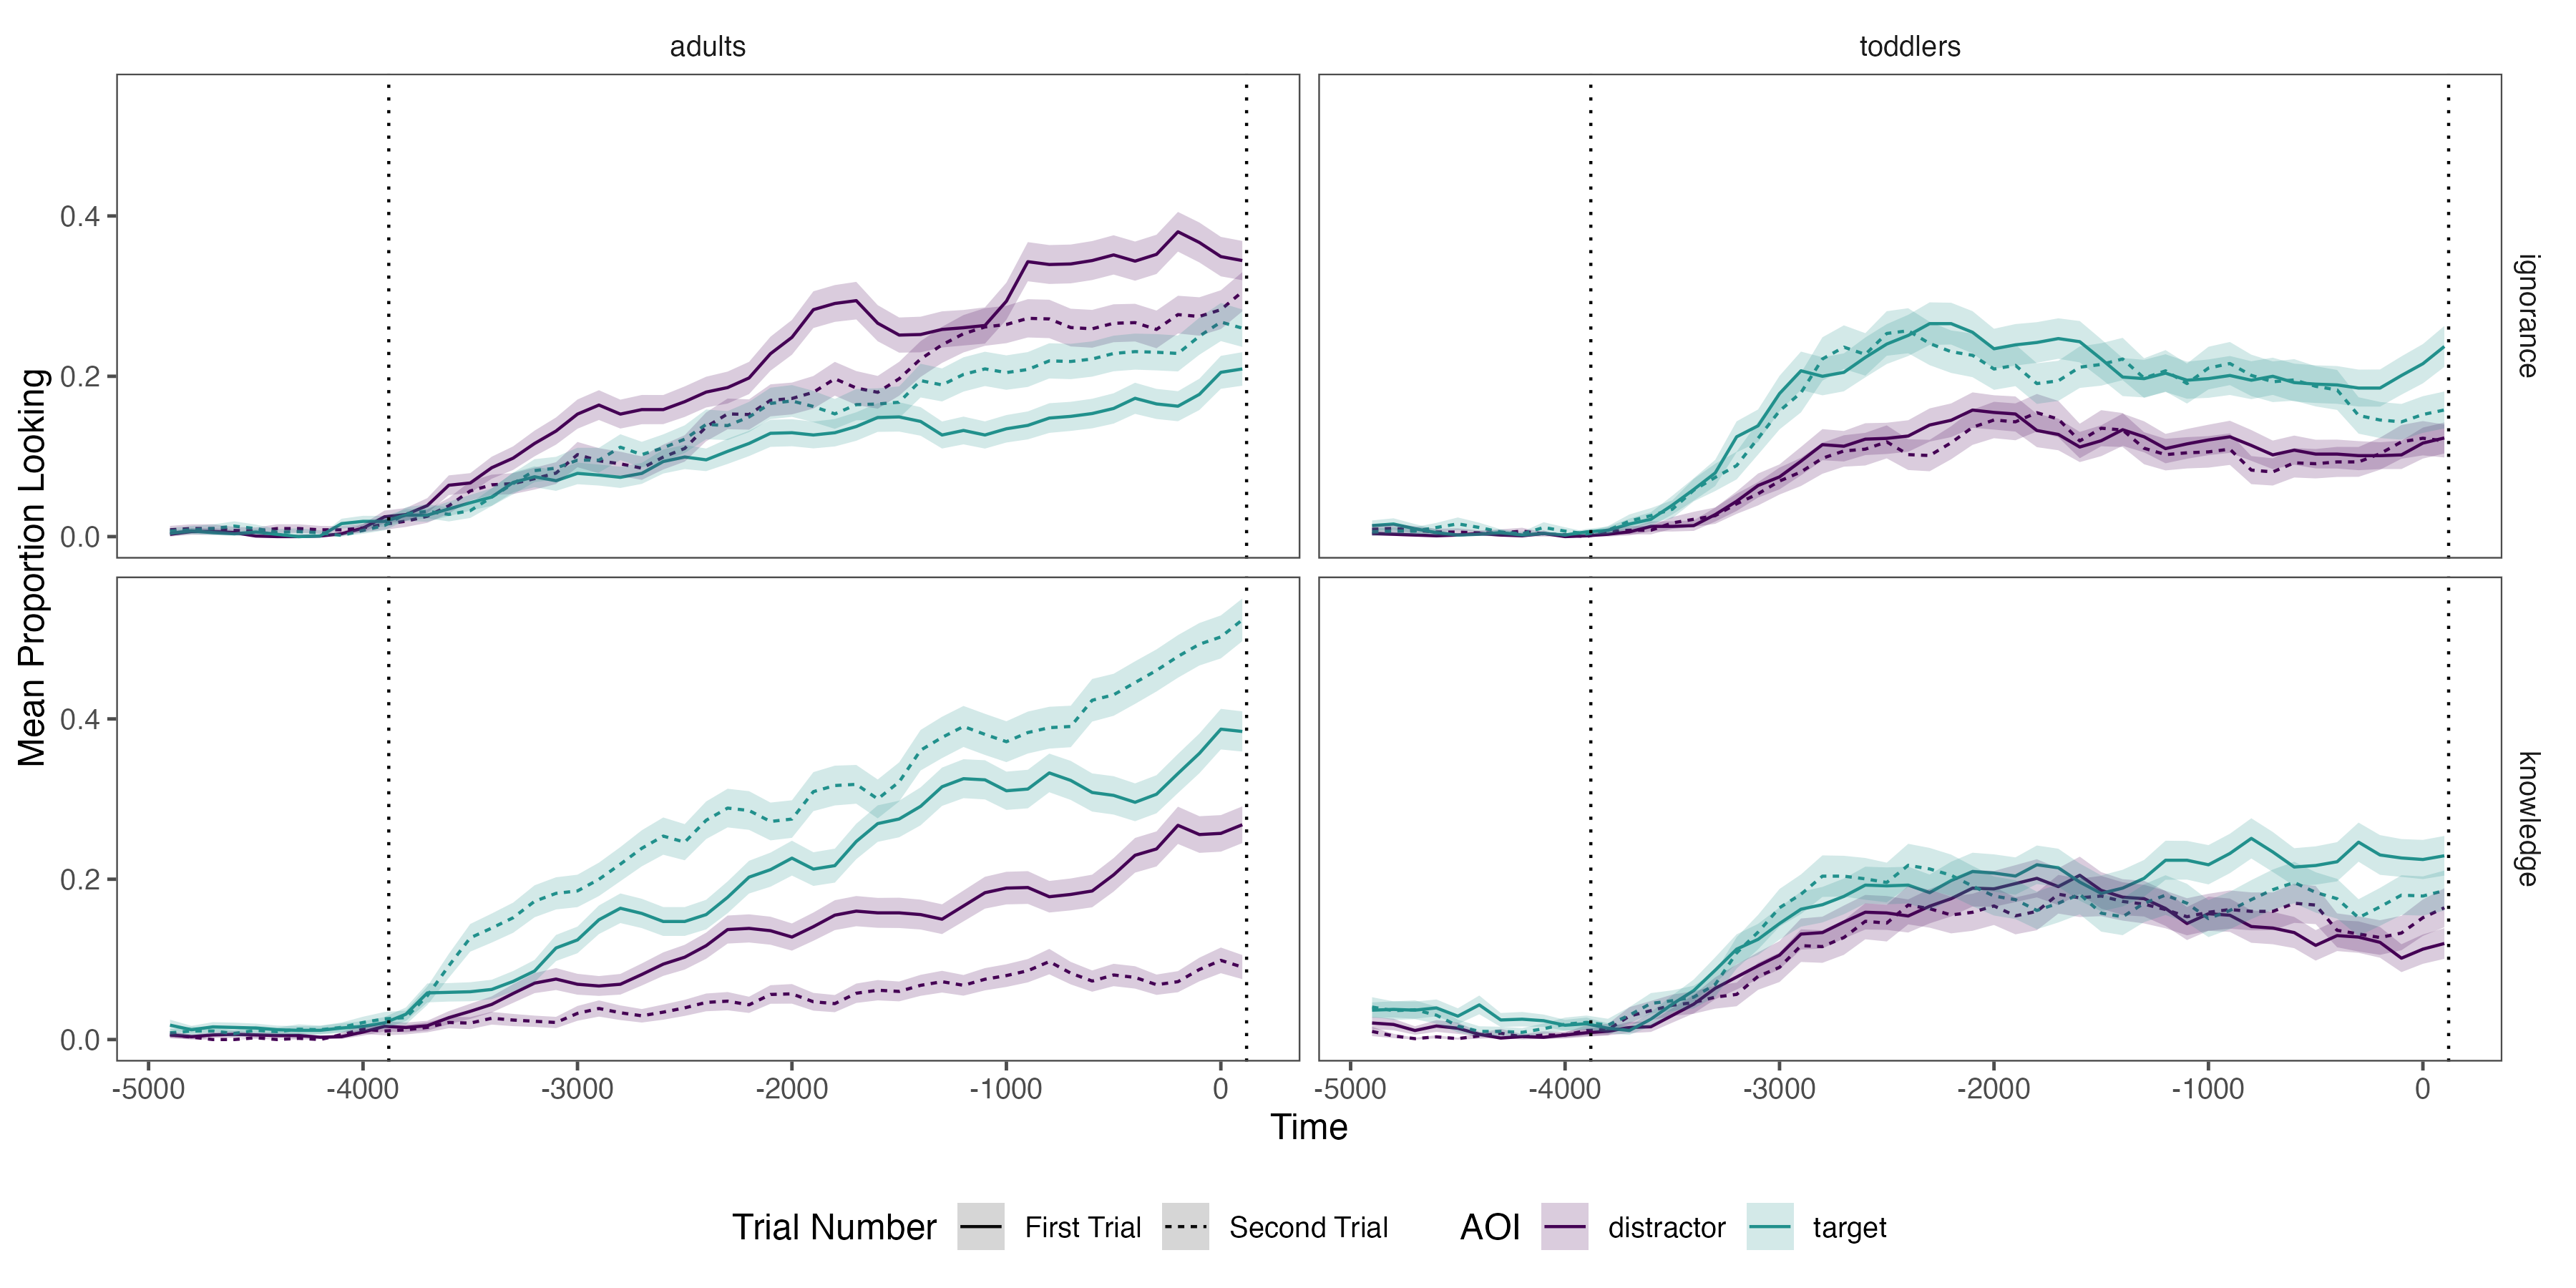
\includegraphics[width=6.8in]{/Users/mellischreiner/Documents/GitHub/mb2-analysis/paper/Figure_test_timecourse_plot_anticipation_phase} 

}

\caption{Timecourse of mean proportional looking for the first and second test trial for toddlers and adults in the ignorance and knowledge condition.}\label{fig:fig5}
\end{figure}

Figure 5 depicts mean proportion of looking to target and distractor during the anticipation window. The timecourse plot displays mean proportional looking for both conditions, knowledge and ignorance, both age cohorts, toddlers and adults, as wells as both test trials, first and second.

\subparagraph{Toddlers}\label{toddlers-3}

As first model, we used a Bayesian mixed effects models to predict toddlers' PTL based on condition, age, and the interaction of condition and age, while accounting for variability across labs. The Bayes factor comparing this model to the simpler null model without the interaction of condition was estimated to be BF = 21.2, favoring the full model over the null model. Table 4 shows the statistics for regression coefficients of the full model. These results suggest a significant effect of condition on PTL, with the positive coefficient indicating higher PTL for ignorance trials compared to knowledge trials.

Additionally, we assessed whether toddlers' AL changed with age. Comparing our full model, which included an interaction between age and condition, with a simpler model without this interaction yielded a Bayes factor, BF = 0.4, providing only anecdotal evidence supporting the simpler model. This result suggests that the interaction between age and condition might not be a necessary predictor, as it doesn't provide substantial additional explanatory power. Hence, our results do not provide sufficient evidence to determine whether age-related changes in AL are consistent across conditions or differ between them.

\subparagraph{Adults}\label{adults-3}

Next, we used a Bayesian mixed effects model to predict PTL based on condition for adults, again with random effects for lab. The Bayes factor comparing this model to the simpler null model without the main effect of condition was estimated to be BF \textgreater{} 1000, strongly favoring the full model over the null model. These results suggest a significant main effect of condition on PTL, with the negative coefficient indicating a higher number of target looks for knowledge than for ignorance trials.

\subsection{Exploratory Analyses}\label{exploratory-analyses}

\subsubsection{Spill-over}\label{spill-over}

We will analyze within-participants data from the second test trial that participants saw, using exploratory models to assess whether (1) findings are consistent when both trials are included (overall condition effect), (2) whether effects are magnified or diminished on the second trial (order main effect), and (3) whether there is evidence of ``spillover'' - dependency in anticipation on the second trial depending on what the first trial is (condition x order interaction effect; see Figure 6).

Analyzing condition-effects of within-participants data for both test trials, we fitted a Bayesian mixed-effects model with the dependent variable of PTL and main effects of condition and age and their interaction for toddlers. Comparing this full model to a null model that did not include the fixed effect of condition, we obtained a Bayes Factor of BF \textless{} 0.1, providing
strong evidence in favor of the null model.

For adults, we also fitted a Bayesian mixed-effects model to predict their PTL for both test trials with the main effect of condition and random effects for participant and lab. Again, the data provided very strong evidence for the inclusion of the main effect of condition with a Bayes Factor of BF \textgreater{} 1000. The effect of condition was negative and credible, suggesting that PTL was significantly lower in the ignorance condition compared to the knowledge condition.

In order to investigate whether there was an interaction of condition and test trial number, we fitted Bayesian mixed-effects models to predict PTL with fixed effects for condition, test trial number, and their interaction, along with random intercepts and slopes for these variables across labs, for toddlers and adults separately. For toddlers, the Bayes factor, BF = 0.4, provided anecdotal evidence for the simpler null model without the interaction term, indicating that the interaction between condition and test trial number does not add substantial explanatory power to the model. These results suggest that neither condition nor its interaction with test trial number significantly impacts PTL in this sample.

For adults, the Bayes Factor, BF = 19.7, provided strong evidence for including the interaction of condition and test trial number as a fixed effect. These results indicate that while PTL increased over trials, this effect was moderated by condition, with the ignorance condition showing a slower rate of increase compared to the knowledge condition.

To examine whether anticipatory looking during the second test trial was influenced by condition and anticipatory looking during the first test trial, we fitted a Bayesian mixed-effects model for each age cohort separately. This model included fixed effects for condition, proportion of target looking during the first test trial, and their interaction. Random intercepts and slopes for these predictors were modeled at the lab level. For toddlers, the Bayes factor, BF = 1.1, suggests negligible evidence in favor of including these predictors compared to the null model, indicating that these factors did not strongly influence second trial anticipatory looking in toddlers. There was a small and non-significant positive main effect of condition, indicating minimal differences in anticipatory looking between conditions and a negligible and non-significant effect of first test trial anticipatory looking. The interaction between condition and first test trial anticipatory looking was also minimal and non-significant. These findings indicate that condition, first trial anticipatory looking, and their interaction did not strongly predict anticipatory looking during the second test trial in toddlers. The Bayes factor close to 1 reflects weak or inconclusive evidence for the inclusion of these predictors, suggesting that the variability in second trial behavior arose from other unmodeled factors.

For adults, the Bayes factor, BF \textgreater{} 1000, strongly supports the inclusion of these predictors, suggesting that condition and first trial behavior substantially explained second trial anticipatory looking. The regression results showed a significant negative main effect of condition, indicating reduced anticipatory looking in the ignorance condition compared to the knowledge condition. There was a small negative effect of first trial anticipatory looking, suggesting that higher anticipatory looking in the first test trial was slightly associated with reduced looking in the second test trial.
The interaction between condition and first test trial anticipatory looking was negligible and non-significant. These findings indicate that condition strongly impacts anticipatory looking during the second test trial, while anticipatory looking during the first trial had a smaller and more nuanced influence. The interaction between condition and first trial looking appears minimal. The extremely large Bayes factor underscores the importance of considering these predictors in explaining second test trial anticipatory looking behavior.

\begin{figure}

{\centering 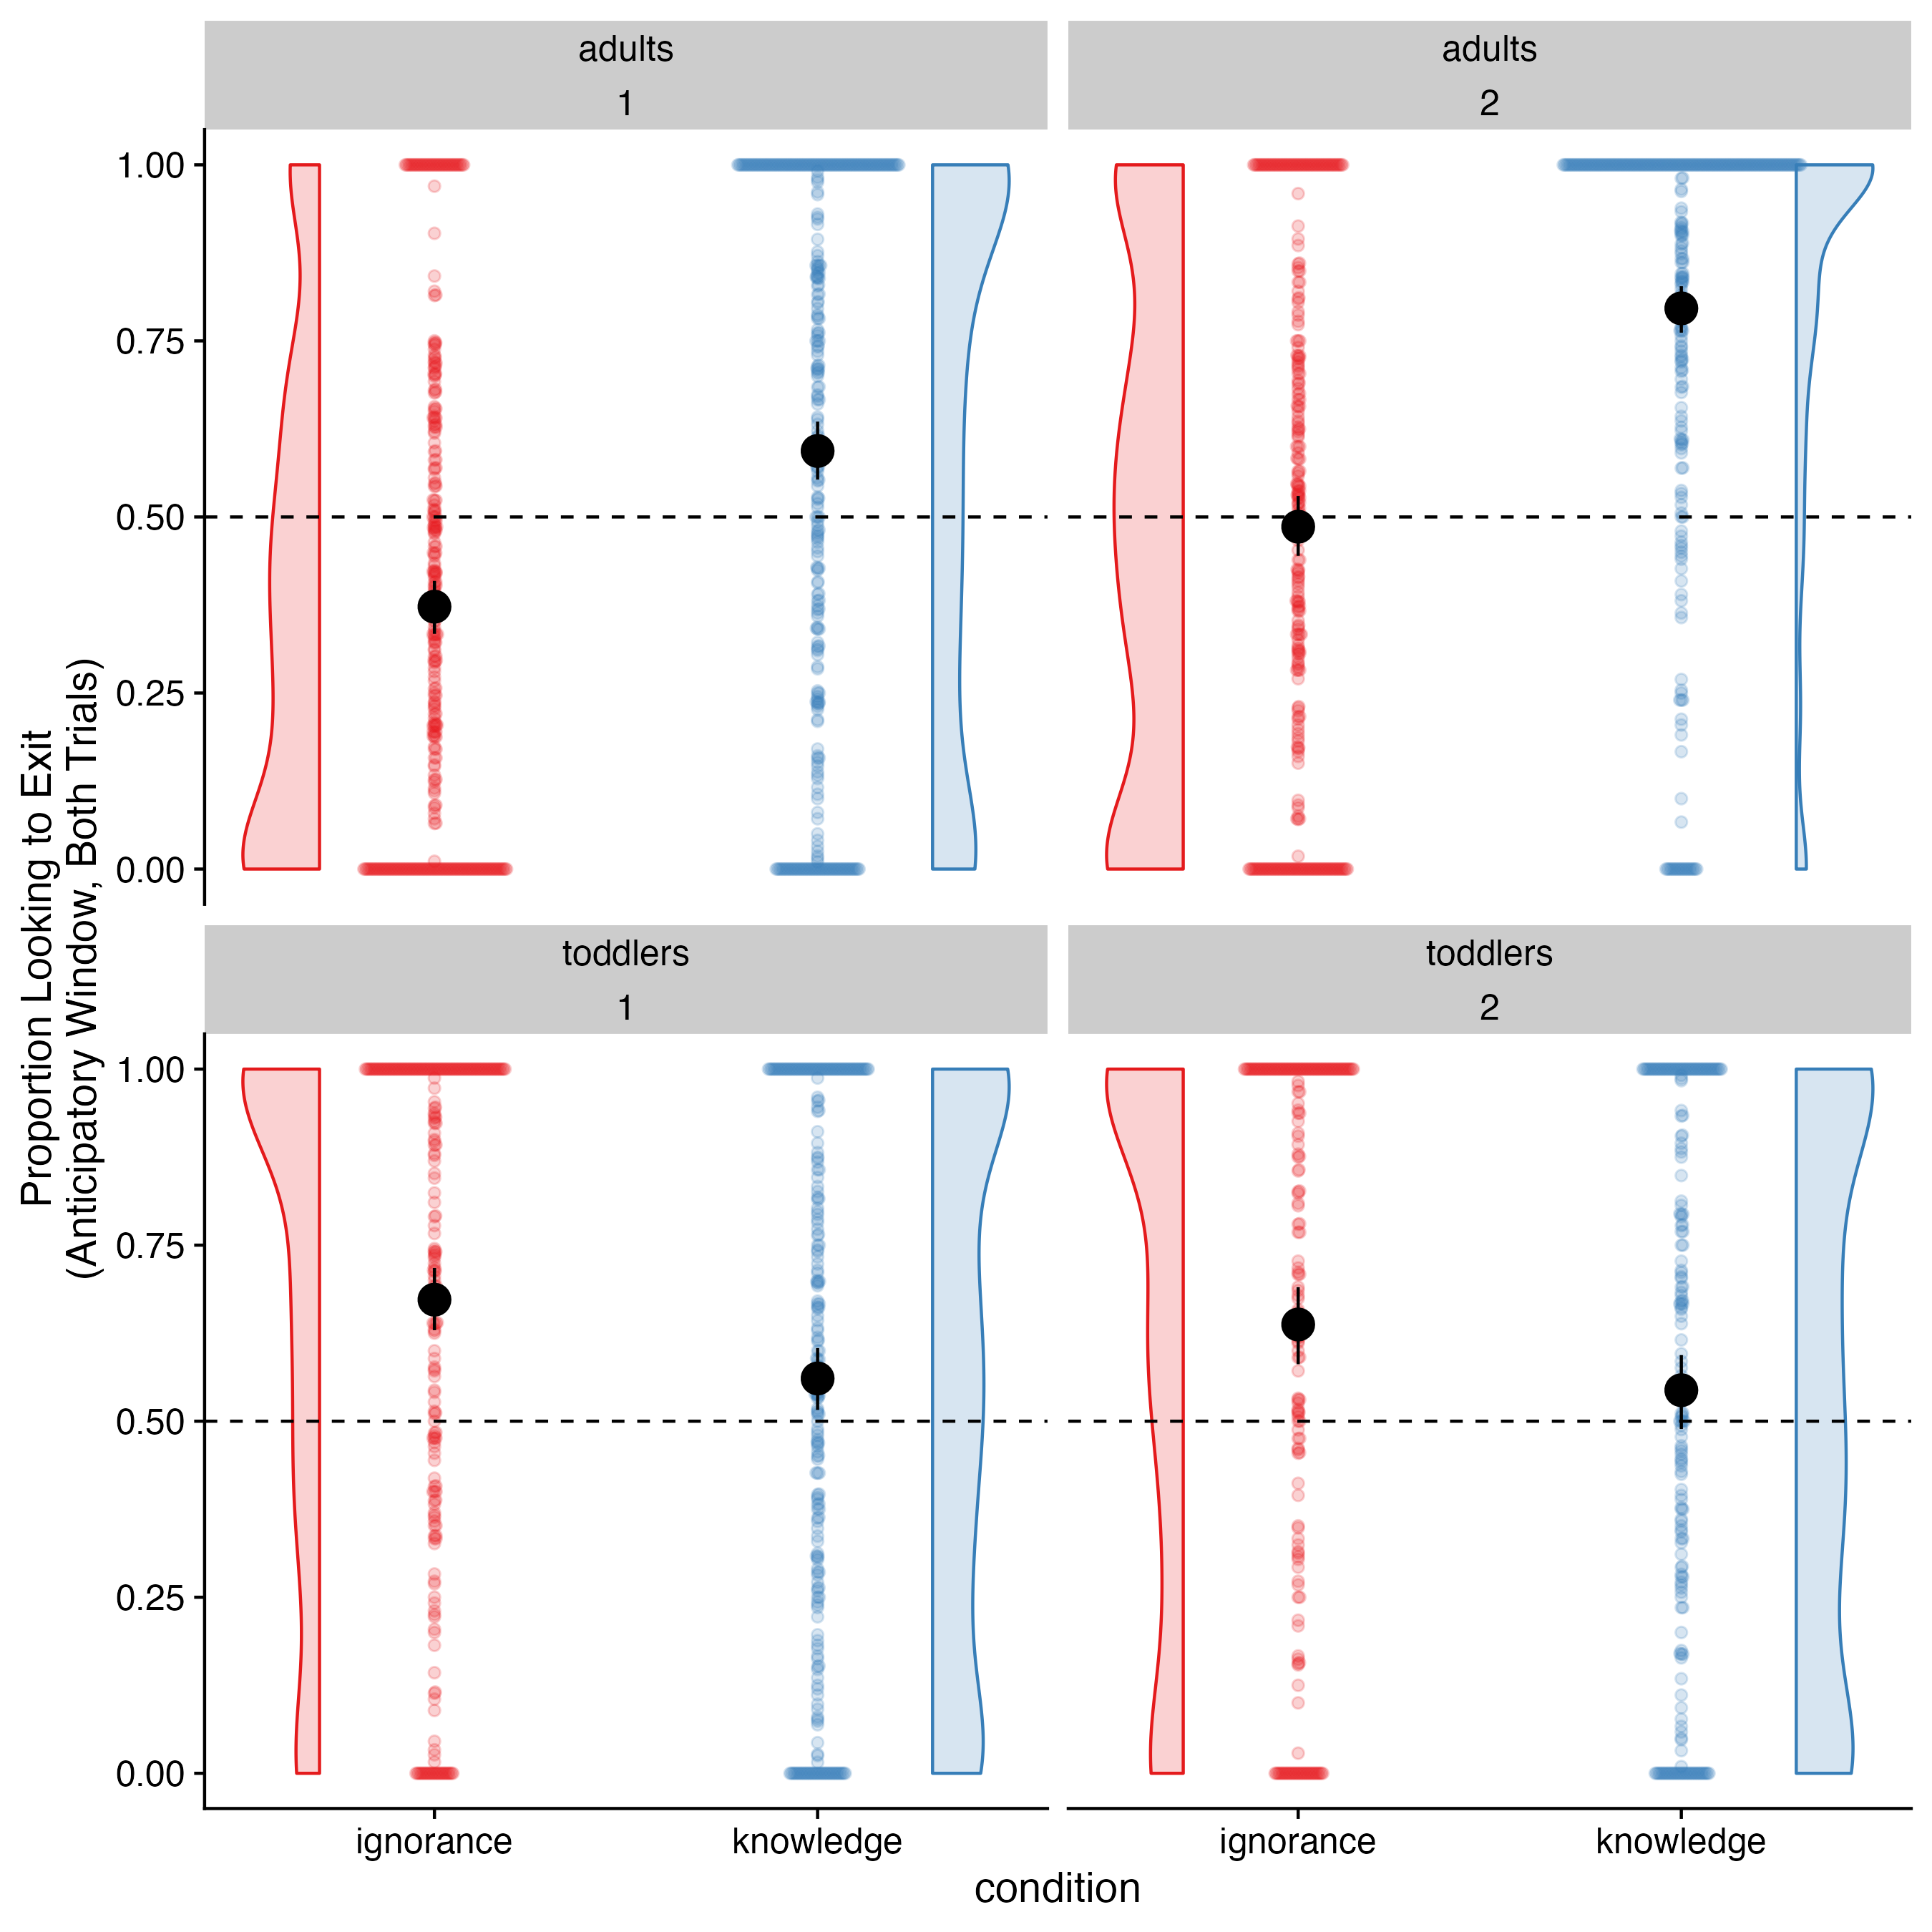
\includegraphics[width=6.8in]{/Users/mellischreiner/Documents/GitHub/mb2-analysis/paper/Figure_PTL_bothtrials} 

}

\caption{Proportional target looking for the first and second test trial for toddlers and adults in the ignorance and knowledge condition.}\label{fig:fig6}
\end{figure}

\subsubsection{Relationship between familiarization and test}\label{relationship-between-familiarization-and-test}

\begin{center}
\begin{ThreePartTable}

\scriptsize{

\begin{longtable}{llrrrrr}\noalign{\getlongtablewidth\global\LTcapwidth=\longtablewidth}
\caption{\label{tab:Results table of Bayesian regression models fam test relationship}Results of the Bayesian mixed effects models for the relationship between familiarization and test.}\\
\toprule
model & \multicolumn{1}{c}{term} & \multicolumn{1}{c}{estimate} & \multicolumn{1}{c}{est\_error} & \multicolumn{1}{c}{lower\_ci} & \multicolumn{1}{c}{upper\_ci} & \multicolumn{1}{c}{rhat}\\
\midrule
\endfirsthead
\caption*{\normalfont{Table \ref{tab:Results table of Bayesian regression models fam test relationship} continued}}\\
\toprule
model & \multicolumn{1}{c}{term} & \multicolumn{1}{c}{estimate} & \multicolumn{1}{c}{est\_error} & \multicolumn{1}{c}{lower\_ci} & \multicolumn{1}{c}{upper\_ci} & \multicolumn{1}{c}{rhat}\\
\midrule
\endhead
adults sufficient familiarization & Intercept & 0.48 & 0.02 & 0.44 & 0.51 & 1.00\\
 & Condition & -0.20 & 0.03 & -0.26 & -0.14 & 1.00\\
 & Successful Fam Anticipation & 0.04 & 0.03 & -0.02 & 0.10 & 1.00\\
 & Condition:Successful Fam Anticipation & 0.00 & 0.05 & -0.11 & 0.10 & 1.00\\
toddlers sufficient familiarization & Intercept & 0.61 & 0.02 & 0.56 & 0.65 & 1.00\\
 & Condition & 0.10 & 0.04 & 0.02 & 0.17 & 1.00\\
 & Successful Fam Anticipation & 0.03 & 0.04 & -0.04 & 0.11 & 1.00\\
 & Condition:Successful Fam Anticipation & 0.02 & 0.06 & -0.11 & 0.14 & 1.00\\
adults correct first look & Intercept & 0.48 & 0.02 & 0.45 & 0.52 & 1.00\\
 & Condition & -0.20 & 0.03 & -0.26 & -0.13 & 1.00\\
 & Correct First Look Final Fam & -0.04 & 0.03 & -0.10 & 0.03 & 1.00\\
 & Condition:Correct First Look Final Fam & -0.08 & 0.06 & -0.19 & 0.04 & 1.00\\
toddlers correct first look & Intercept & 0.62 & 0.02 & 0.58 & 0.65 & 1.00\\
 & Condition & 0.07 & 0.04 & 0.00 & 0.15 & 1.00\\
 & Correct First Look Final Fam & 0.00 & 0.04 & -0.07 & 0.07 & 1.00\\
 & Condition:Correct First Look Final Fam & -0.05 & 0.06 & -0.17 & 0.07 & 1.00\\
\bottomrule
\end{longtable}

}

\end{ThreePartTable}
\end{center}

We will explore whether condition differences vary for participants who show higher rates of anticipation during the four familiarization trials. For example, we might group participants according to whether they did or did not show correct AL at the end of the familiarization phase, defined as overall longer looking at the correct AOI than the incorrect AOI on average in trials 3 and 4 of the familiarization phase.

To investigate whether participants who show anticipatory looking during the familiarization phase also exhibit anticipatory looking during the test phase, we explored three different measures. First, we assessed anticipatory looking in participants who successfully anticipated during the final familiarization trial, defined as those whose first fixation was on the target. Second, we examined anticipatory looking in participants who consistently demonstrated anticipatory behavior across all familiarization trials, operationalized as having a PTL greater than 0.5 in each trial. Finally, we computed correlations to explore whether performance in the familiarization phase was related to performance in the test trials.

\paragraph{Relationship between anticipatory looking during the first test trial and first look during final familiarization trial}\label{relationship-between-anticipatory-looking-during-the-first-test-trial-and-first-look-during-final-familiarization-trial}

We fitted a main Bayesian hierarchical model testing the fixed effects of condition (ignorance vs.~knowledge), first look during the final familiarization trial (target vs.~distractor), and their interaction on first-trial proportion target looking during the anticipatory window for toddlers and adults separately. Random intercepts and slopes for all fixed effects and their interaction were included at the lab level, accounting for variability across different experimental settings.
For toddlers, the Bayes factor comparing this model to the simpler null model without the interaction of condition and first look during the final familiarization trial indicated that the data slightly favored the simpler null model over the full model, BF = 0.7. The effect of condition was positive, but its confidence interval narrowly included zero, suggesting weak evidence for a condition effect (see Table 5). The effect of performance during the final familiarization trial was close to zero, indicating no substantial main effect of prior performance. Similarly, the interaction between condition and performance in the final familiarization trial was small and non-significant. These results suggest that while there was some weak evidence for a main effect of condition on anticipatory looking, neither performance during the final familiarization trial nor its interaction with condition substantially predicted anticipatory looking during the test trial. This result indicates that the relation between anticipatory looking during the first test trial and condition did not depend significantly on prior familiarization performance.

For adults, the Bayes factor comparing this model to the simpler null model without the main effect of condition was estimated to be BF \textgreater{} 1000, strongly favoring the base model over the null model. The regression coefficients showed a significant negative effect of condition, indicating that anticipatory looking was lower in ignorance trials compared to knowledge trials. The decisive Bayes factor strongly favors the inclusion of condition and familiarization trial performance in the model, suggesting that these predictors are relevant for understanding anticipatory looking in adults. However, the small and non-significant estimates for the effects of familiarization trial performance and its interaction with condition imply that condition is the primary driver of anticipatory looking differences, with performance in familiarization trials contributing minimally.

\paragraph{Only \textgreater50\% looking to target during familiarization trials}\label{only-50-looking-to-target-during-familiarization-trials}

To examine the effect of condition and successful anticipatory looking during familiarization (above 50\% target looking during all familiarization trials) on anticipatory looking during the first test trial, we fitted Bayesian mixed-effects models for each age group separately. The models included fixed effects for condition, anticipatory looking during familiarization trials, and their interaction. Random intercepts and slopes for these predictors were included at the lab level. Comparing the full model to the null model of toddlers revealed a Bayes Factor of BF = 10.9, providing strong evidence favoring the full model over a null model that excludes these predictors, suggesting that these factors contribute meaningfully to explaining the variance in test trial anticipatory looking. The regression analysis showed a positive main effect of condition, indicating higher anticipatory looking in one condition compared to the other (see Table 5). There was a small positive, but non-significant, effect of successful anticipatory looking during familiarization. The interaction between condition and successful anticipatory looking during familiarization was also small and non-significant. These results indicate that condition is a meaningful predictor of anticipatory looking during test trials in toddlers, with participants showing different levels of anticipatory looking based on condition. However, the successful anticipatory looking during familiarization trials and its interaction with condition appear to have minimal additional impact. The strong Bayes factor further supports the importance of including these predictors in the model but highlights that condition remains the primary driver of test trial differences.

The estimated Bayes factor in favor of the full model of adults over the null model was BF \textgreater{} 1000, indicating that the predictors substantially contribute to explaining test trial anticipatory looking. The regression coefficients revealed a significant main effect of condition, with participants showing lower anticipatory looking in the ignorance condition compared to the knowledge condition. There was a small, positive, and non-significant effect of successful anticipatory looking during familiarization and the interaction between condition and successful successful anticipatory looking during familiarization was negligible. These results indicate that condition has a substantial and meaningful impact on anticipatory looking during the first test trial in adults, while successful anticipatory looking in familiarization trials and its interaction with condition have limited additional influence. The extremely large Bayes factor highlights the strong explanatory power of including these predictors in the model, although condition remains the primary driver of the observed differences.

\paragraph{Correlation between familiarization and test}\label{correlation-between-familiarization-and-test}

\begin{figure}

{\centering 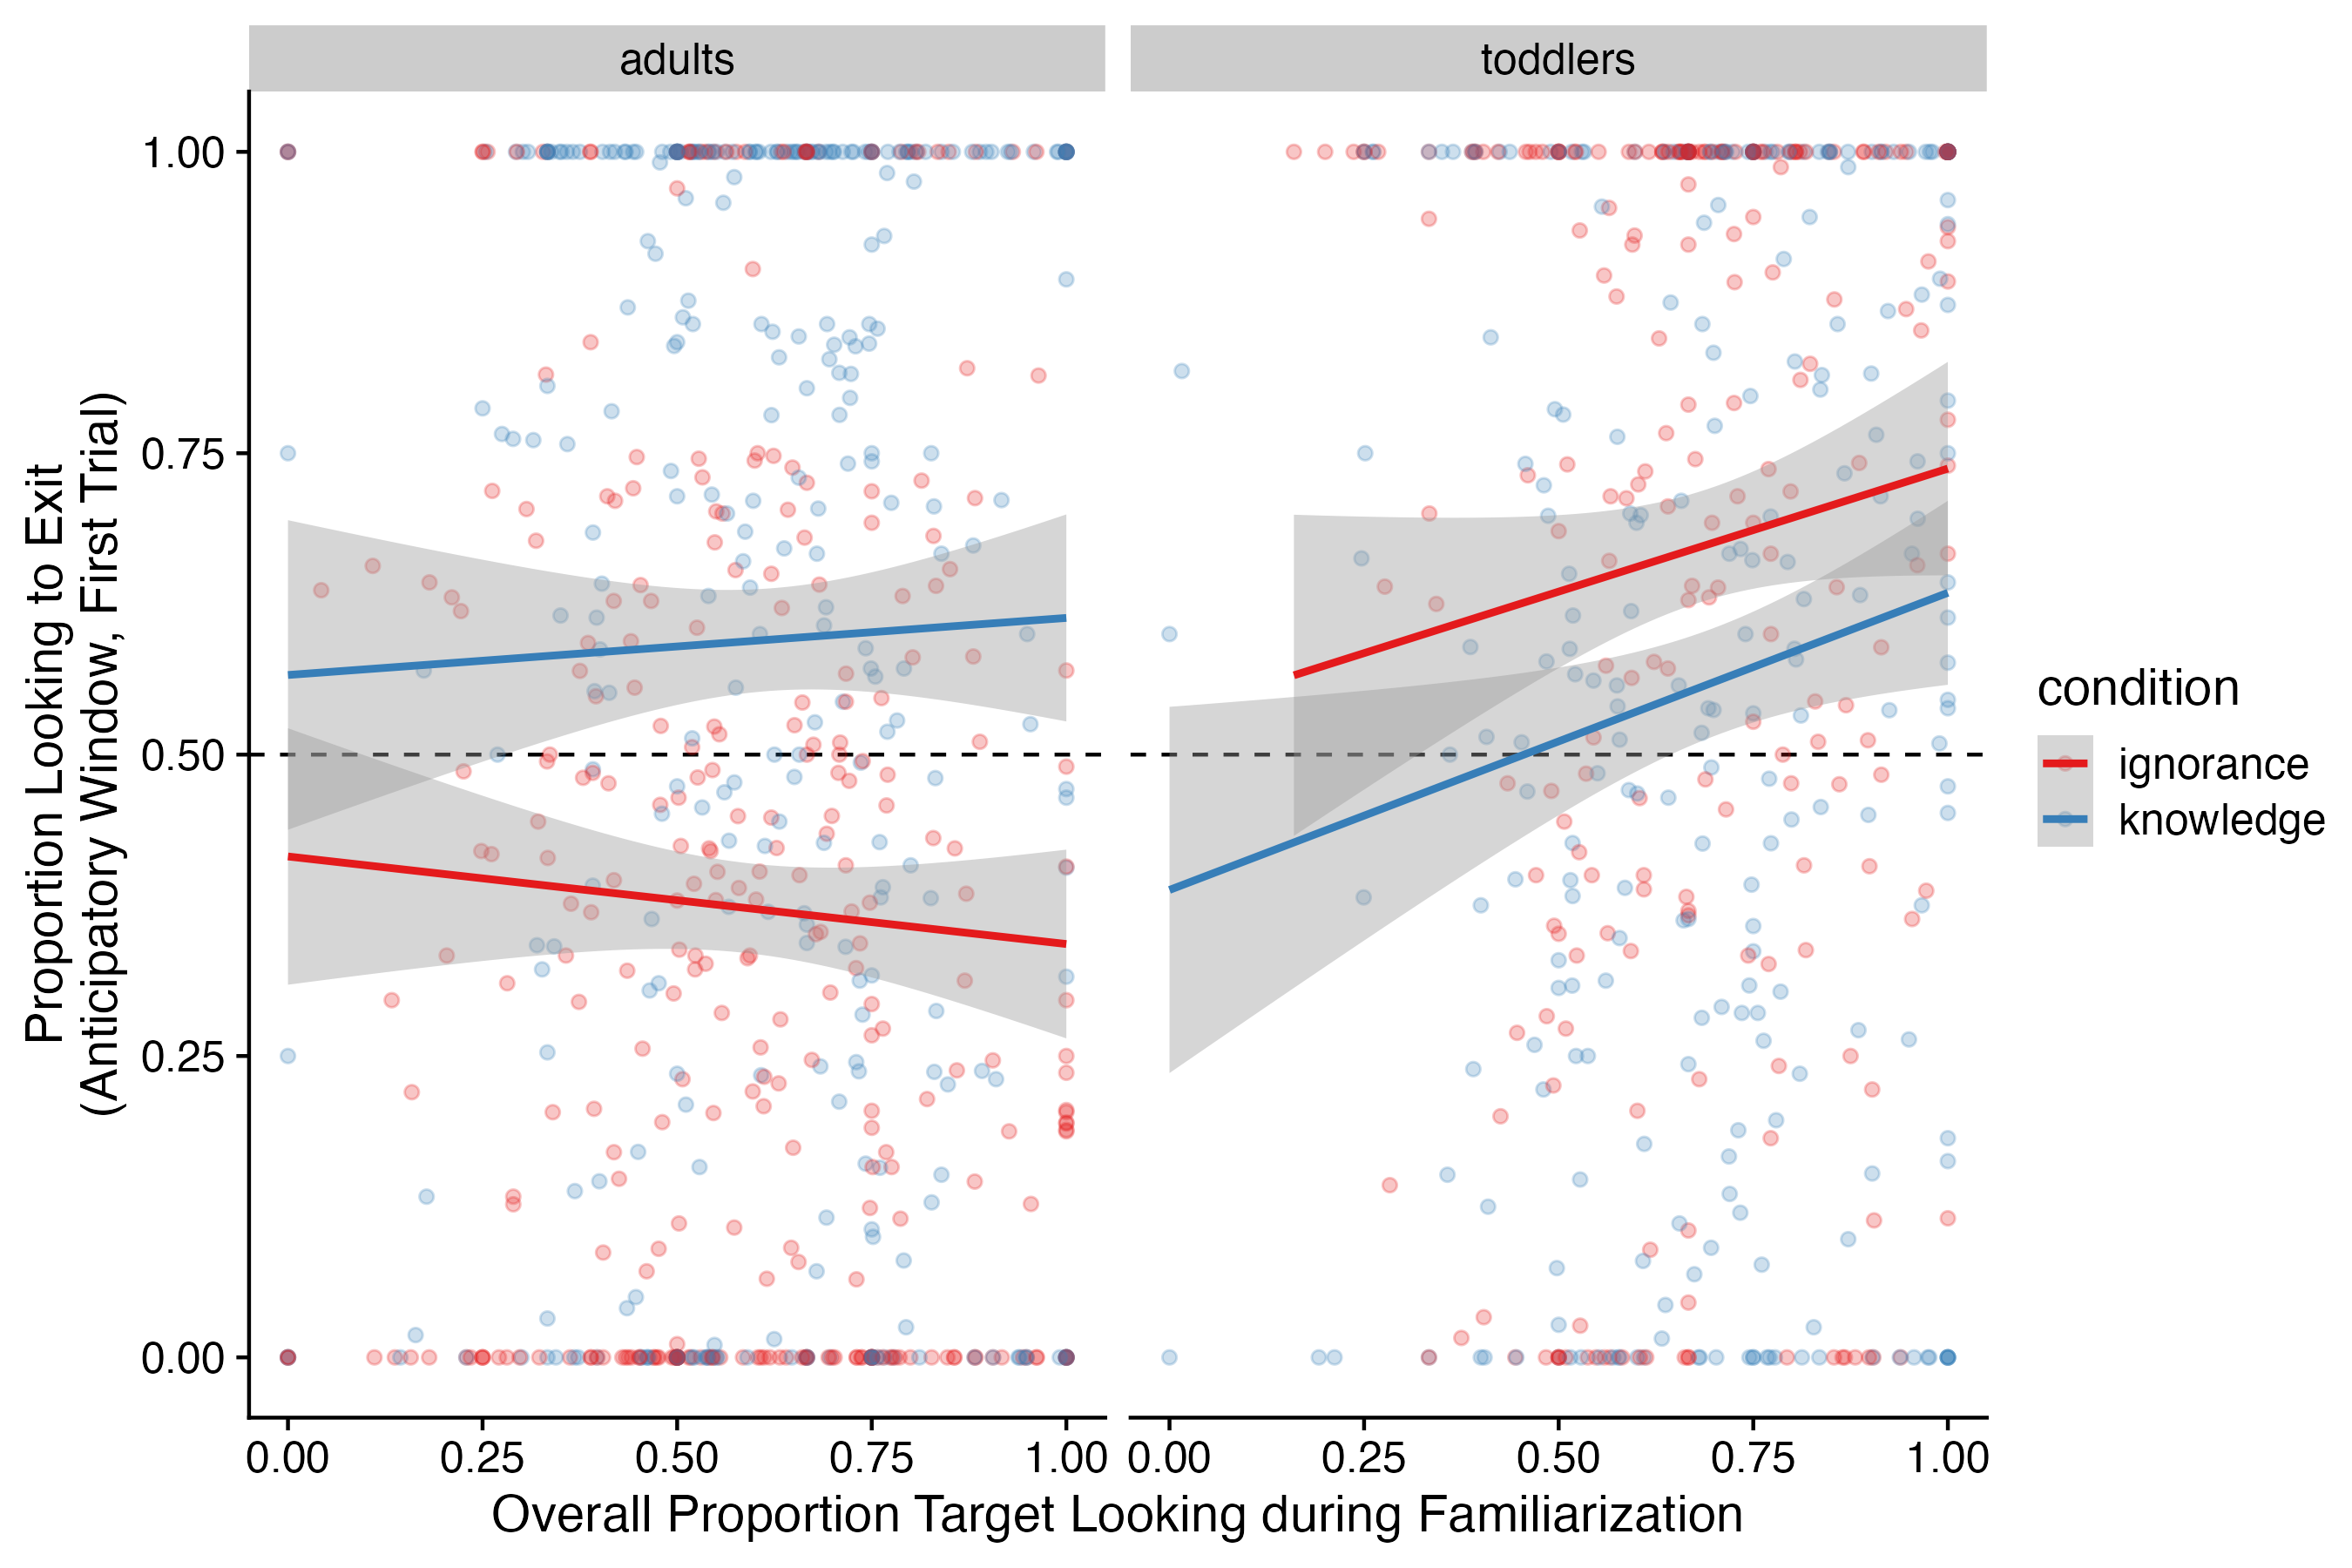
\includegraphics[width=6.8in]{/Users/mellischreiner/Documents/GitHub/mb2-analysis/paper/correlation_plot_fam_test} 

}

\caption{Relationship of anticipatory looking during familiarization and test for both age cohorts and conditions.}\label{fig:fig7}
\end{figure}

We also examined the correlation between familiarization and test performance across the two age cohorts and conditions (see Figure 7). While no significant correlations were found for adults in either condition, toddlers in the knowledge condition exhibited a significant positive correlation of anticipatory looking in familiarization and test, \emph{r}=0.15, \emph{t}(254)=2.35, \emph{p}=0.02, suggesting that toddlers, who showed higher proportional target looking overall during familiarization, also showed higher proportional target looking in the first test trial. No such significant correlation was found for toddlers in the ignorance condition , \emph{r}=0.11, \emph{t}(234)=1.68, \emph{p}=0.09. However, there was also no significant interaction between condition and the correlation in anticipatory looking between familiarization and test for toddlers (p = .79).

\subsubsection{Looking patterns during mouse's change of location.}\label{looking-patterns-during-mouses-change-of-location.}

To examine whether participants monitored both the bear and the mouse during the mouse's location change, and whether this influenced AL in the test phase, we defined new time windows of interest (TOIs) corresponding to the mouse's location change in each condition and new AOIs for both the mouse and bear. We hypothesized that participants who attended to both AOIs would exhibit greater AL compared to those who predominantly tracked the mouse during its location change. Specifically, we analyzed the frequency of gaze shifts between the mouse and bear mouse's location change. An additional exploratory analysis of differential gaze duration directed toward mouse and bear during the mouse's location change is provided in the Supplement S3.

\paragraph{Comparing the number of shifts of toddlers and adults during the location change of the mouse.}\label{comparing-the-number-of-shifts-of-toddlers-and-adults-during-the-location-change-of-the-mouse.}

We fitted a Bayesian mixed-effects model to examine the relationship between the number of shifts between mouse and bear and age cohort during location change of the mouse, while accounting for random effects by lab. The effect of condition was negative and approached significance, suggesting a potential reduction in the number of shifts for the ignorance condition compared to the knowledge condition. The main effect of age cohort was positive and credible, Estimate=0.56, indicating that the number of shifts was higher for adults than for toddlers. Importantly, the interaction between condition and age cohort was negative and credible, indicating that the negative effect of condition was more pronounced in the adult cohort (see Figure 8).
Comparing this model to a simpler model without the interaction of condition and age cohort, a Bayes Factor of BF \textgreater{} 1000 was computed.
This provides strong evidence in favor of including the interaction of condition and age cohort in the model.

\begin{figure}

{\centering 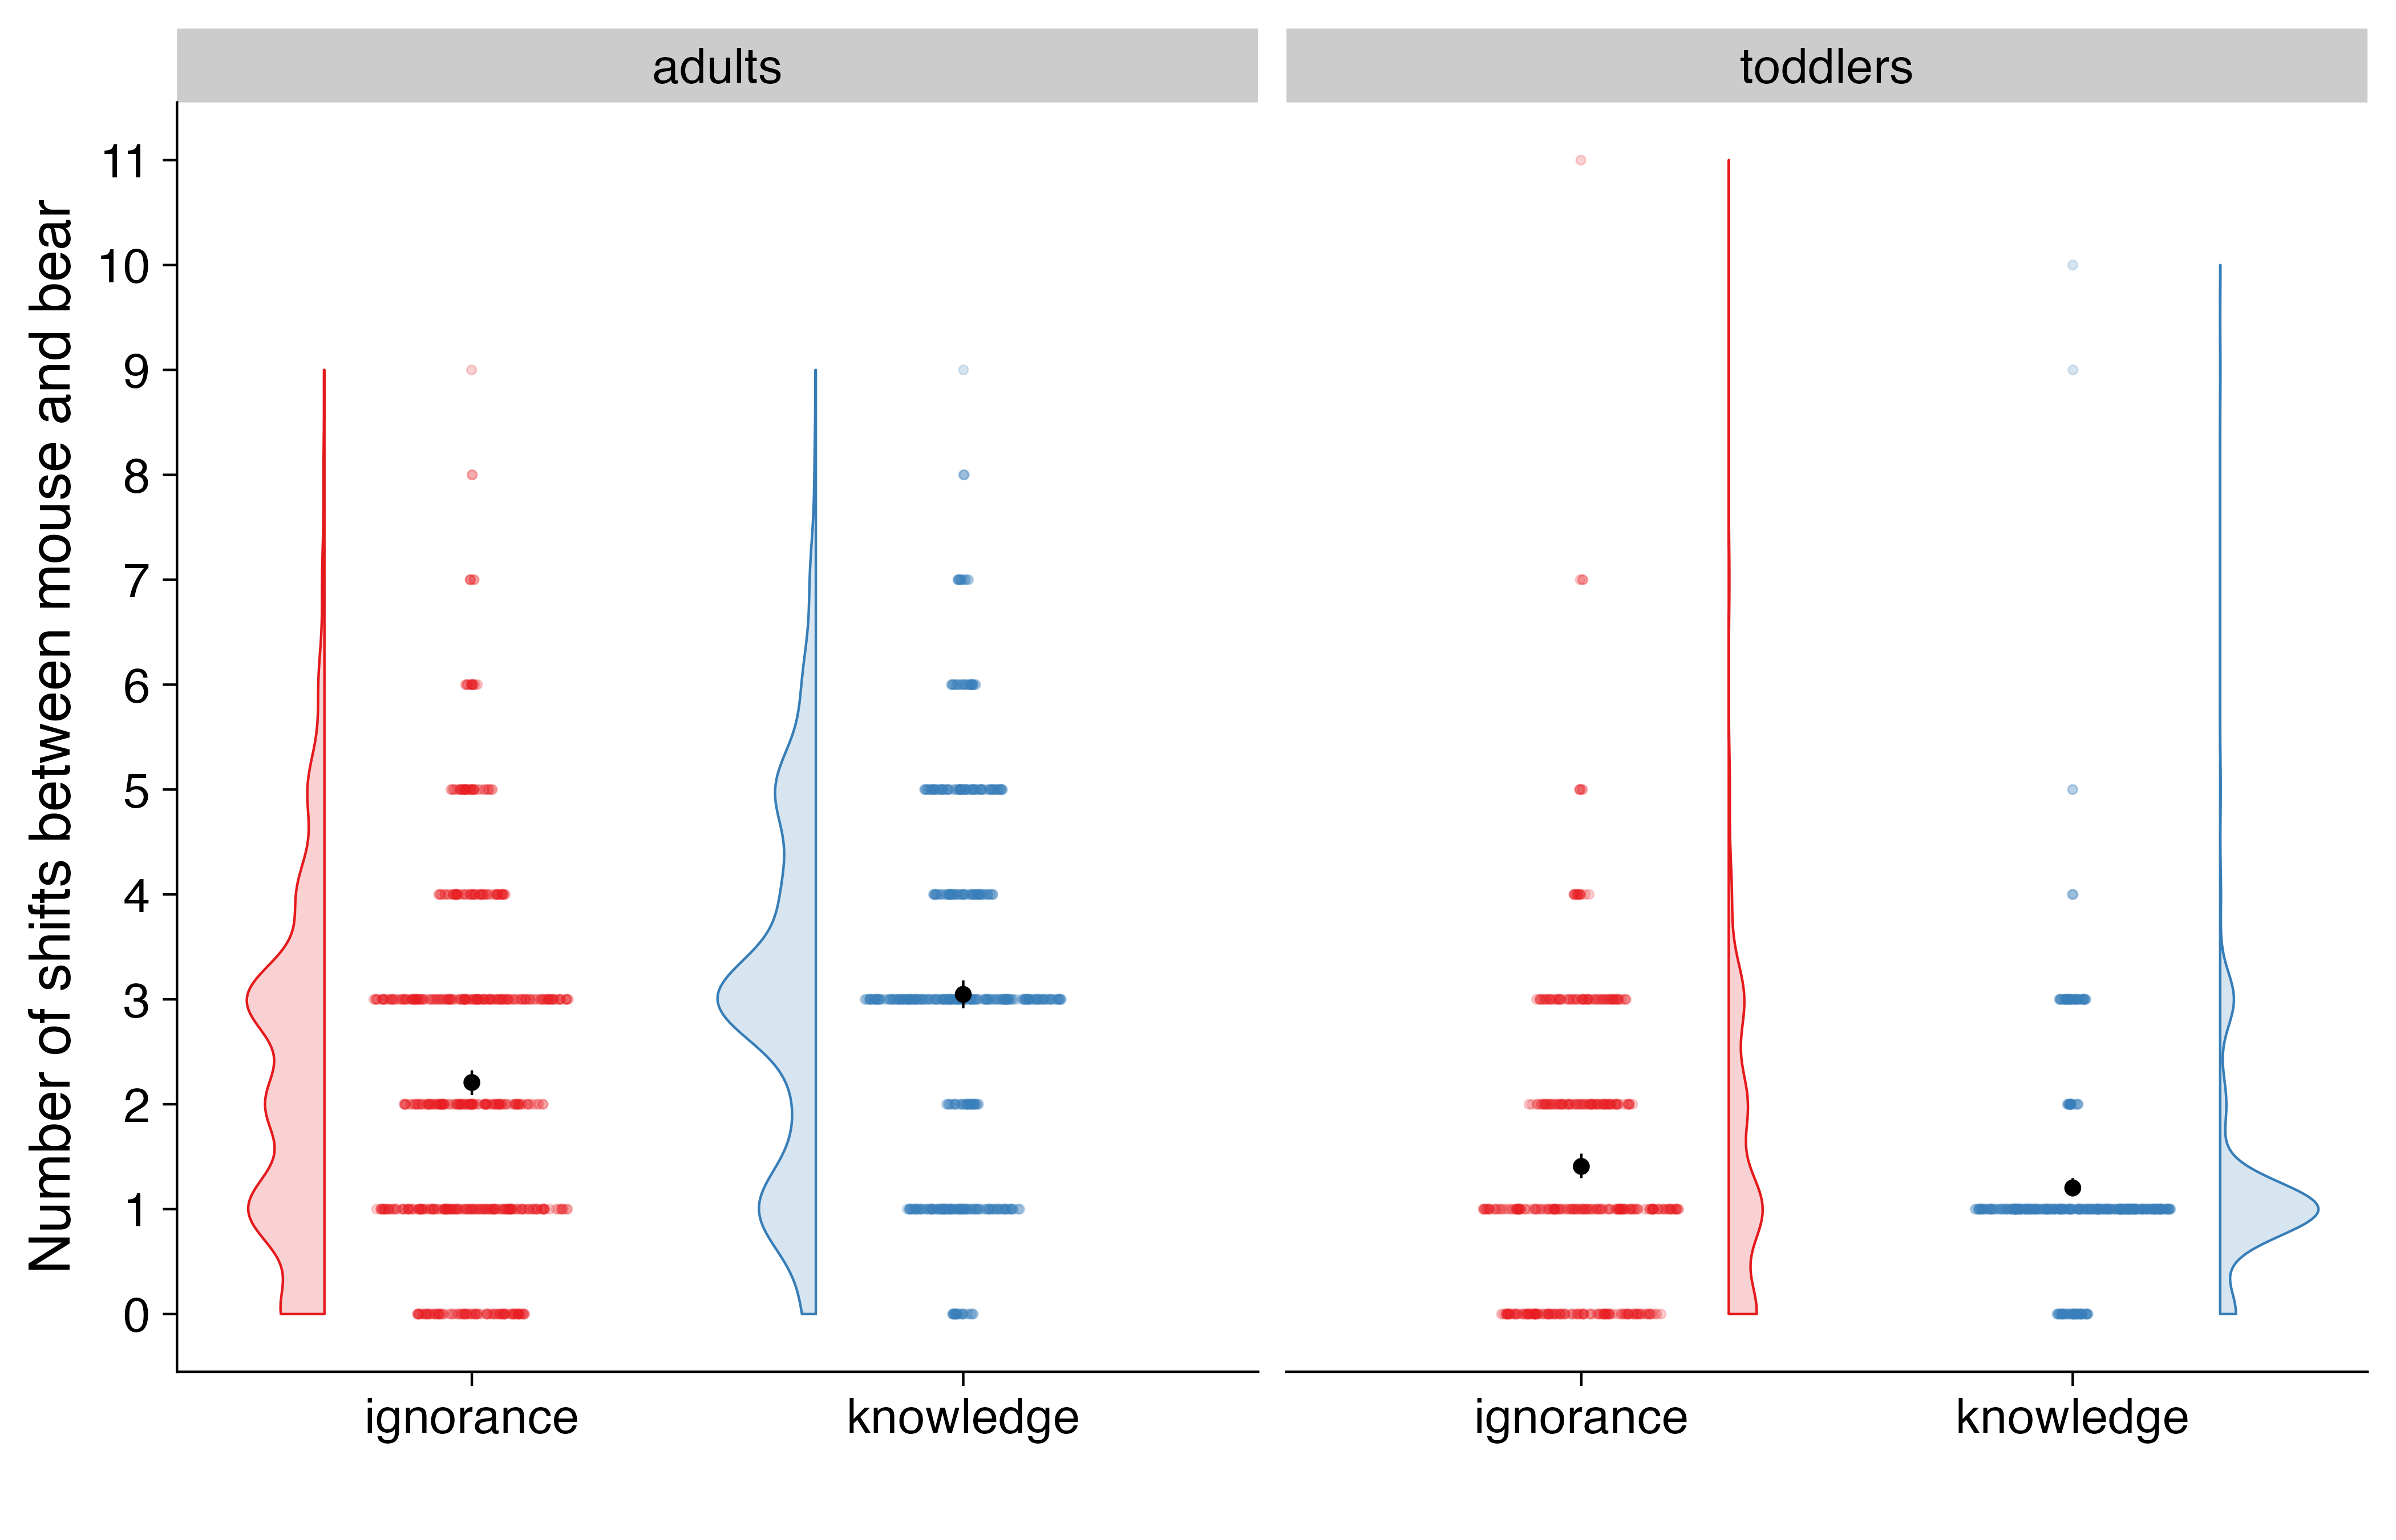
\includegraphics[width=6.8in]{/Users/mellischreiner/Documents/GitHub/mb2-analysis/paper/Figure6b} 

}

\caption{Number of shifts between mouse and bear during location change of mouse in the test phase for toddlers and adults in the ignorance and knowledge condition.}\label{fig:fig8}
\end{figure}

\paragraph{AL as a function of number of gaze shifts between mouse and bear during location change}\label{al-as-a-function-of-number-of-gaze-shifts-between-mouse-and-bear-during-location-change}

In order to examine the effect of condition and the number of shifts between mouse and bear during location change of the mouse on anticipatory looking, we fitted Bayesian mixed-effects models for each age cohort separately (see Figure 9). The dependent variable was PTL in the anticipation period. The fixed effects included the main effects of condition, the number of shifts, and their interaction. We also included random intercepts and slopes for number of shifts within each participant and within each lab, allowing us to account for the hierarchical structure of the data and potential variability between labs and participants.

For toddlers, comparing this model to a simpler model without the interaction of condition and number of shifts, a Bayes Factor of BF \textless{} 0.1 was computed, indicating that the data strongly favors the null model over the full model. This suggests that the predictors number of shifts and the interaction with condition included in the full model do not improve the explanation of the observed data compared to the null model.

For adults, the number of shifts showed a small but credible positive effect, suggesting that more shifts were associated with an increase in PTL. The interaction between condition and the number of shifts was negative and credible, indicating that the effect of condition became more negative as the number of shifts increased. The estimated Bayes factor comparing the full model to the null model was approximately BF \textgreater{} 1000, providing strong evidence in favor of the full model over the null model.

\begin{figure}

{\centering 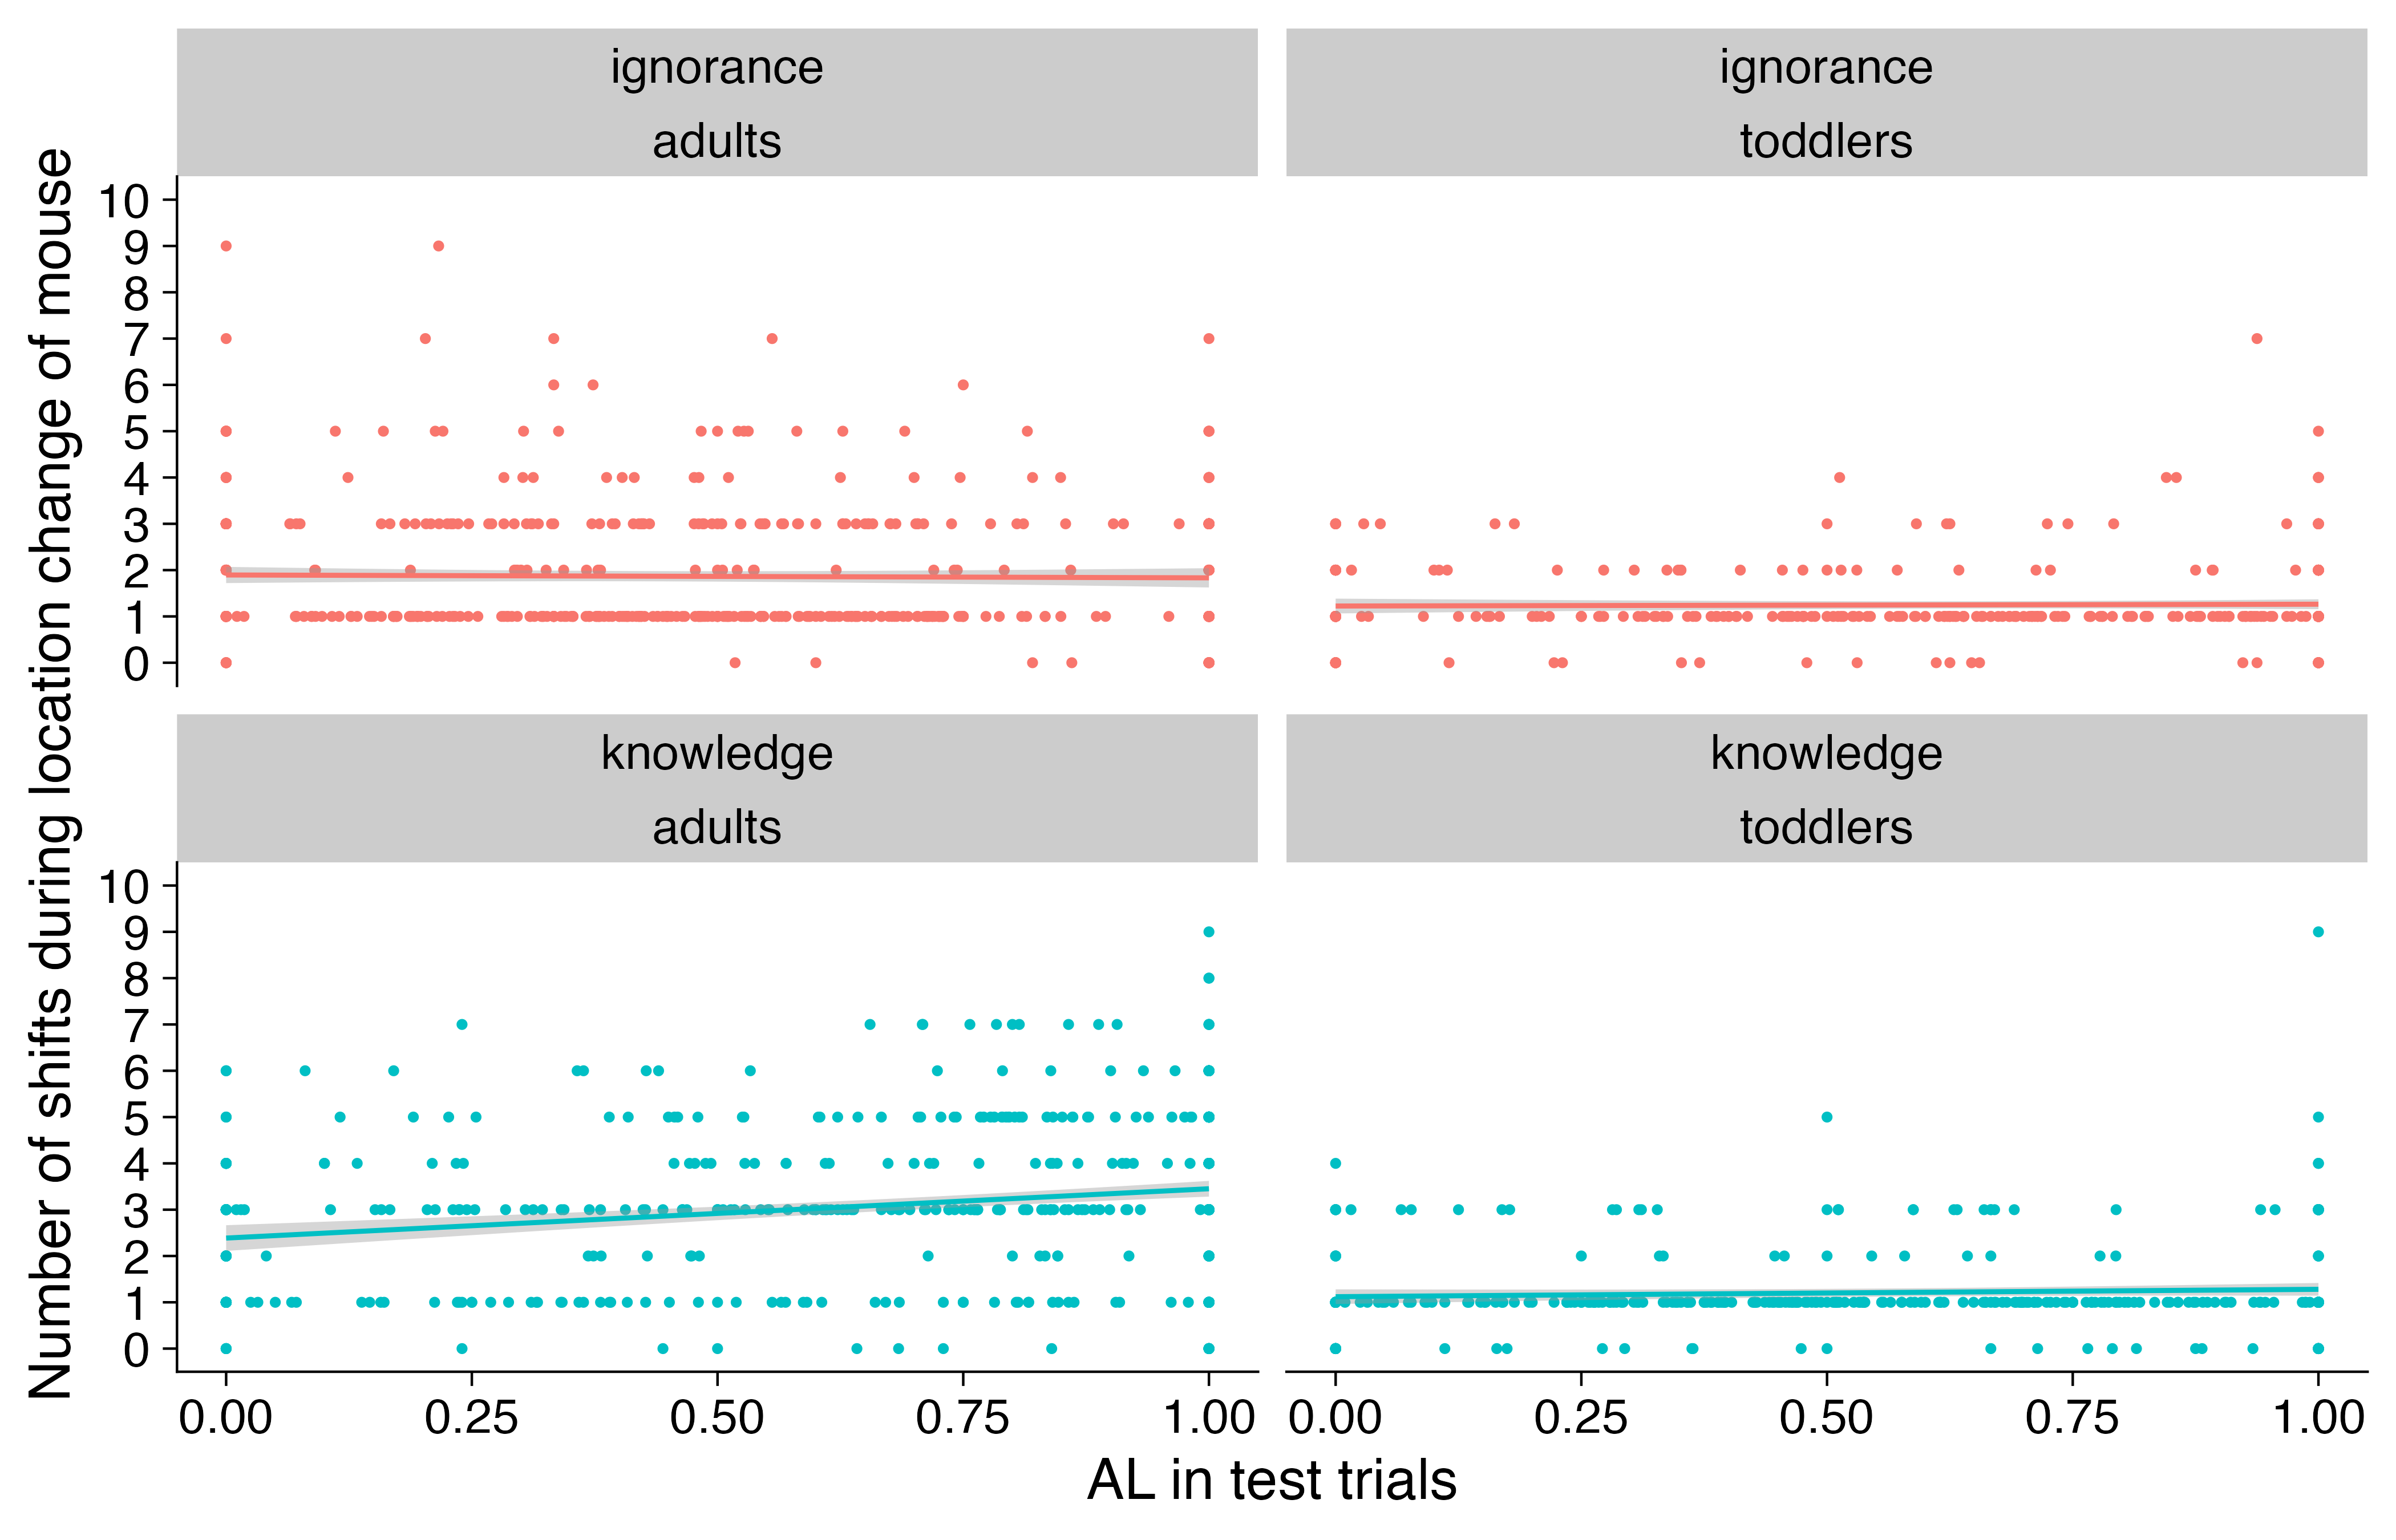
\includegraphics[width=6.8in]{/Users/mellischreiner/Documents/GitHub/mb2-analysis/paper/Figure7} 

}

\caption{AL as a function of number of shifts between mouse and bear during location change of mouse in the test phase for toddlers and adults.}\label{fig:fig9}
\end{figure}

\section{General Discussion}\label{general-discussion}

The overarching aim of the ManyBabies 2 consortium is to investigate the robustness and replicability of studies showing spontaneous Theory of Mind from infancy across the lifespan. The first project, the initial steps of which are reported here, takes a systematic, sequential bottom-up approach to address anticipatory looking as a measure of spontaneous Theory of Mind and pursues three objectives. First, we aim to develop stimulus material (i.e., videos) that reliably and generally elicits spontaneous, goal-based action anticipation -- such that young children and adults look where an agent will go as a function of their goal. In this way, the problem of very high exclusion rates in previous studies (of children who did not spontaneously anticipate) could be overcome (e.g., Kampis et al., 2020; Kulke, Reiß, et al., 2018; Schuwerk et al., 2018; Southgate et al., 2007). If the first goal can be met, the second goal is to examine whether young children and adults demonstrate action anticipation that is sensitive to basic epistemic states of agents: do they anticipate as a function of whether the agent has or has not seen crucial events and is thus knowledgeable or ignorant of them? If the second goal can be fully met, the third goal, to be addressed in future work, is to test the replicability of the original findings of the false belief/true belief contrast. In this paper, we focused on the first two steps and laid the foundation for future work on the third.
\#\# Summary and evaluation of main findings
Concerning our first goal, the present work was successful. In two pilot studies (see Supplement S1) and the main study reported here, toddlers and adults reliably engaged in spontaneous goal-based action anticipation: they looked ahead of time towards the location where an agent would go, given their goal. This licensed the conclusion that the present stimulus material is suitable for studying spontaneous action anticipation and laid the foundation for addressing the second goal in the main study: is spontaneous action anticipation sensitive to the agent's epistemic status?
The results of this study were mixed, even with the large sample size of more than 500 toddlers and 700 adults tested in over 30 labs around the world. By accounting for random effects due to lab, our modeling approach allows us to generalize our findings to toddlers and adults across diverse socio-cultural and lab contexts.
Adults showed clear evidence of the anticipatory looking patterns that one would expect if they engaged in action anticipation that is sensitive to the agent's epistemic status. When the agent (chaser) witnessed the crucial events in the Knowledge condition and thus knew where the target (chasee) was, adults looked in anticipation towards the corresponding location. This anticipation was indicated by both first looks and proportional looking time. When the chaser did not witness the crucial event in the Ignorance condition and thus did not know where the chasee was, they did not show such a pattern of anticipatory looking and rather looked at the tunnel exit opposite of the chasee's actual location. Supporting this interpretation, there were clear condition differences in both the first-looks measure and proportion of anticipatory looking.
For toddlers, the findings were different and puzzling. They tended to show qualitatively the same anticipatory looking (both in first looks and in proportional looking time) towards the target location in both Knowledge and Ignorance trials. The qualitative result in the Knowledge condition is consistent with adult behavior. Yet quantitatively, children anticipated substantially more in the Ignorance compared to the Knowledge condition in their proportion of anticipatory looking-- precisely the reverse effect of what one would expect if children tracked the agent's epistemic status.
The overall picture that the present study presents is thus the following: The findings with adults were straightforward and in line with our predictions. In their anticipatory looking, adults engaged in spontaneous goal-based action anticipation (pilot studies and main study), and in doing so, they took into account the agent's epistemic status (main study). Based on this, the next step would be to pursue the third goal: testing whether adults take into account true/false beliefs of an agent in their spontaneous action anticipation. Specifically, adults are expected to anticipate that the agent will go to the actual location of the target in the true belief condition but to the location where the agent falsely believes the target to be in the false belief condition (e.g., Schneider et al., 2012; Senju et al., 2009).
In contrast, the findings with the toddlers are puzzling and not in line with our predictions. Although toddlers did engage in spontaneous goal-based action anticipation (pilot studies and main study), they did not show clear evidence of taking into account the agent's epistemic status (main study) in the way adults did.
\#\# Big open question: How can the puzzling looking patterns in toddlers be explained?
The puzzle is what to make of these findings with children. How did the surprising anticipatory looking pattern of children come about? Why did toddlers not anticipate more clearly the chaser's action in the Knowledge condition? And why did they show anticipatory looking to the box with the chasee in the Ignorance condition (where they should not do so, or at least to a lesser degree)? A number of initially plausible explanations could be ruled out via exploratory analyses. One such explanation was that behind the grouped data, more nuanced sub-group patterns were hidden. For example, older children could be performing as expected, while younger children were not; or children who anticipated strongly in the familiarization trials could be performing as expected, while children who showed little or no anticipation were not. However, corresponding exploratory analyses along these lines did not find compelling evidence for such sub-group patterns. Neither toddlers' age nor anticipatory looking in the familiarization trials had an effect on the pattern of test trial results. Another explanation was that perseveration from the last familiarization trial to the first test trials (such that children persevere in looking in anticipation to the location they have previously looked to) differentially affected Knowledge and Ignorance conditions and could thus account for at least parts of the puzzling pattern. But the relevant exploratory control analyses (for details see Supplemental Material) did not find any convincing evidence for such a possibility.
How then can these puzzling anticipatory looking patterns in the Knowledge vs.~Ignorance conditions in toddlers be explained? More specifically, how can we explain why toddlers in the Ignorance condition engaged in strong anticipatory looking towards the unpredicted location (where the chasee currently is, unbeknownst to the chaser)? And how can we explain why they showed only very weak correct action predictions in the Knowledge condition -- weaker than in the Ignorance condition, and weaker than in the familiarization trials? We discuss several possibilities below. These are currently all, needless to say, post hoc speculations. But they may lay the foundation for testing them in future studies.
\#\#\# Timing differences between conditions
One possibility regarding the Ignorance condition is that slight differences in timing between the conditions may have posed challenges for toddlers. Specifically, in the Ignorance condition, the chaser hides at the back and fails to witness the key events where the chasee moves first to one box and then to another. In contrast, in the Knowledge condition, the chaser observes the chasee going to one box, then leaves, returns and witnesses how the chasee moves between the boxes (see Figure 2). As a result, the conditions differed subtly in timing. In the Ignorance condition, there was a slightly longer interval between the initial hiding event at location 1 and the anticipatory looking phase. This extended interval may have impaired children's memory of the event, making location 1 less salient and leading them to focus more on location 2 during the anticipation phase. Although the lack of an age effect between 18- and 27-month-olds slightly undermines the memory-capacity explanation (because increasing memory capacity in this age interval should have produced an effect of age), future studies could address this issue by equating the temporal structures of both conditions.
\#\#\# Attentional and other processing demands
A second possible explanation for the obtained pattern of results, and in particular, why toddlers did not anticipate more clearly and strongly in the Knowledge condition, may relate to attentional and other processing demands of the Knowledge and Ignorance conditions.
Regarding attention, the Knowledge condition raises particular demands of distributing and coordinating attentional focus. In the familiarization trials, children show clear and strong goal-based action anticipation. However, in these trials, the chaser remains present in the scene all the time (it never goes towards the back), and the chasee goes to one box in the chaser's presence but does not change to the other box. In the Knowledge test trials, in contrast, there is much more going on: the chaser leaves towards the back and then returns, and the chasee first goes to one box, and then relocates to the other. Perhaps dividing attention between the relevant events (chaser is at the back, chasee at the same time in one box) and coordinating it over time (keeping track of what the chaser has witnessed when) was too demanding for toddlers, and as a result they lost track of the narrative structure of the events. Exploratory analyses of gaze shifts between chaser and chasee in toddlers vs.~adults may be seen as an indication that there is something to this explanation: Adults seemed to track the chaser's perceptual access, as indicated by many gaze shifts between chaser and chase during the location change. In contrast, toddlers' attention remained largely on the moving chasee with fewer gaze shifts towards the chaser who was witnessing the relocation in the Knowledge condition. Future studies could test more directly whether attentional demands made the present Knowledge condition particularly demanding. The chaser could be continuously present all the time, for example, and never leave towards the back (which was introduced to keep the Knowledge condition as similar as possible to the Ignorance condition) -- thus reducing the need to divide and coordinate attention between chaser and chasee. The corresponding Ignorance condition could then be realized differently, not such that the chaser leaves, but, for example, such that their view becomes blocked by an occluder, or they falls asleep or is otherwise blindfolded.
Relatedly and more generally, the complexity of the event sequences to be followed and tracked in both conditions may pose excessive performance demands that mask children's competence to understand the agent's epistemic status. Overburdened by such processing demands, toddlers may revert to simpler cognitive strategies influenced by dynamic visual salience, for example. Future research should aim to address these cognitive constraints by further simplifying task demands and optimizing event timing.
\#\#\# Challenges of understanding the implementation of the Ignorance condition
A third possibility is that toddlers' (and adults') anticipation is related to their differing conceptual understanding of the scenes in the Ignorance trials. In the Ignorance condition, the chaser leaves but its back is visible. This requires monitoring and understanding that this does not give the chaser epistemic access to the events, which may overburden toddlers. Additionally, the Ignorance condition presents a challenge regarding what to anticipate: should participants expect that the chaser will come out at one of the two exits at random? Or that the chaser will go to the location where the chase is not? Interestingly, adults' looking behavior in the Ignorance condition suggests that they expected the chaser to go to the incorrect location, similar to what might be predicted in a False-Belief scenario or an ignorance-leads-to-error heuristic (e.g., Ruffman, 1996; but see Friedman \& Petrashek, 2009). Adults and toddlers looked comparably in Knowledge trials with slightly above chance anticipation (albeit stronger in adults), whereas the two groups showed entirely opposite patterns in the Ignorance condition. This raises important questions about how toddlers interpreted the Ignorance condition. Did they entirely lose track of the chaser's epistemic state? Did they show a `pull of the real', focusing on the actual location of the chasee? If so, why did this not occur in the Knowledge condition? Alternatively, they may have been governed by altogether different assumptions about the events in the scene. This raises the possibility that the Ignorance condition may not be the most optimal comparison to the Knowledge condition for toddlers. These concerns could be addressed by exploring alternative implementations of the Ignorance condition, such as those proposed above.
\#\#\# Differential habituation and task construal across trials between the conditions
A fourth possibility, finally, is that toddlers habituated to and construed the events over time differently in the Knowledge and Ignorance conditions. In the Knowledge condition, from toddlers' perspective the first test trial was the fifth trial (after the four familiarization trials) that was similar in the sense that the chaser went to look for the chasee after watching it hide. So they might have simply begun to lose interest in the task. In contrast, no such habituation may have taken place in the Ignorance condition in which the first test trial did differ from the last familiarization trial in that the chaser did not witness the chasee hiding.
In addition, this may have been gone along with a different and very rich construal by toddlers of the events in the first Ignorance test trial: For the first time, in this trial the chaser did not know where to go, and the chasee knew that. Rather than not keeping track of the agents' perspectives on the scene (under-thinking), toddlers may have engaged in very complex reasoning (over-thinking) about such perspectives along the following lines: They may have looked toward the chasee's box because they expected the chasee to signal its hiding location in some way, to help the chaser find it and allow their cooperative game to continue. From this perspective, toddlers thus not only understood the chaser's ignorance, but they expected the chasee to understand it too and to act accordingly. This made the chasee, rather than the chaser, the focus of toddlers' anticipation: They anticipated that the chasee would somehow signal its location, to help the chaser find it. This interpretation of the task also indicates that it may measure something different in toddlers and adults and that anticipatory looking in toddlers can have a different meaning than it has in adults -- i.e.~a lack of measurement invariance (Meredith, 1964). While such a very rich interpretation does not receive any direct support from the present data, it could be put to systematic test in future studies (for example, by having the two agents interact in less cooperative ways).

\subsection{Conclusion and future directions}\label{conclusion-and-future-directions}

The current large-scale study examined the robustness and reliability of studies using anticipatory looking as a measure of spontaneous Theory of Mind in toddlers and adults. The novel stimuli designed for this study reliably elicited spontaneous goal-based action anticipation, as shown in two pilot studies and in the main study. Spontaneous anticipatory looking occurred to a higher degree and resulted in lower exclusion rates than in previous studies - confirming the importance of the baseline checks, especially in replication studies. In this sense, the current study provides robust stimulus material suitable to elicit goal-based AL in both toddlers and adults.
The main study tested whether toddlers and adults, in their spontaneous action anticipation, take into account the epistemic status of an agent who witnesses relevant events and knows where the target is (Knowledge condition) or fails to do so (Ignorance condition). Adults clearly did take into account the agent's epistemic status and distinguished between the Knowledge and the Ignorance condition: they anticipated that the agent would go to the target in the Knowledge, but expected the opposite in the Ignorance condition. In contrast, toddlers showed anticipatory looking to the target location in both conditions, but did so in quantitatively stronger ways in the Ignorance than in the Knowledge condition, which is the reverse as expected.
Future research with adults could build on the present findings, for example, by testing whether adults engage in belief-based action anticipation and thus whether original findings of implicit Theory of Mind in adults can be replicated. Future research with children, in contrast, should first sort out the sources of the unexpected results found here. This will require systematic follow-up studies along several lines: First, the Knowledge-Ignorance condition contrast could be implemented in alternative, ideally simpler, ways as suggested in the above discussion. Second, an interesting extension would be to test whether young children do indicate some understanding of the present Knowledge-Ignorance contrasts in other measures. Anticipatory looking itself may be a demanding measure due to its predictive nature (cf. Johnson, Posner, \& Rothbart, 1991). Postdictive measures, in contrast, such as looking behavior and pupil dilation in response to events that are/are not expected given the agent's Knowledge/Ignorance may be more sensitive to uncover early competence (e.g., Daum, Attig, Gunawan, Prinz, \& Gredebäck, 2012). Currently, a spin-off project (\url{https://manybabies.org/MB2P/}) is running the first follow-up studies in this direction. Finally, looking at children at different ages, for example, older children approaching an age of verbal Theory of Mind reasoning, could shed light on whether their behavior in this task may be related to an underlying conceptual understanding (e.g., Wiesmann et al., 2018). Taken together, these future studies will hopefully shed more light on the reality and robustness of implicit Theory of Mind from infancy to adulthood.
To conclude, this study represents a critical step forward in understanding the development and robustness of spontaneous Theory of Mind across the lifespan. By developing novel, reliable stimuli and implementing a large-scale, multi-lab approach, it has laid the groundwork for replicable research in this domain. The findings demonstrate that adults' anticipatory looking aligns with epistemic sensitivity, while the unexpected, puzzling patterns in toddlers challenge existing assumptions and thus open up exciting new avenues for future research. By addressing these puzzles, this work paves the way for deeper insights into the developmental trajectory of Theory of Mind and the cognitive mechanisms underlying its expression in infancy, childhood, and beyond.

\newpage

\section{References}\label{references}

\begingroup
\setlength{\parindent}{-0.5in}
\setlength{\leftskip}{0.5in}

\phantomsection\label{refs}
\begin{CSLReferences}{1}{0}
\bibitem[\citeproctext]{ref-apperly2009humans}
Apperly, I. A., \& Butterfill, S. A. (2009). Do humans have two systems to track beliefs and belief-like states? \emph{Psychological Review}, \emph{116}(4), 953.

\bibitem[\citeproctext]{ref-baillargeon2018invited}
Baillargeon, R., Buttelmann, D., \& Southgate, V. (2018). Invited commentary: Interpreting failed replications of early false-belief findings: Methodological and theoretical considerations. \emph{Cognitive Development}, \emph{46}, 112--124.

\bibitem[\citeproctext]{ref-baillargeon2010false}
Baillargeon, R., Scott, R. M., \& He, Z. (2010). False-belief understanding in infants. \emph{Trends in Cognitive Sciences}, \emph{14}(3), 110--118.

\bibitem[\citeproctext]{ref-barone2019infants}
Barone, P., Corradi, G., \& Gomila, A. (2019). Infants' performance in spontaneous-response false belief tasks: A review and meta-analysis. \emph{Infant Behavior and Development}, \emph{57}, 101350.

\bibitem[\citeproctext]{ref-barr2013random}
Barr, D. J. (2013). Random effects structure for testing interactions in linear mixed-effects models. Frontiers Media SA.

\bibitem[\citeproctext]{ref-burkner2017brms}
Bürkner, P.-C. (2017). Brms: An r package for bayesian multilevel models using stan. \emph{Journal of Statistical Software}, \emph{80}, 1--28.

\bibitem[\citeproctext]{ref-burnside2018implicit}
Burnside, K., Ruel, A., Azar, N., \& Poulin-Dubois, D. (2018). Implicit false belief across the lifespan: Non-replication of an anticipatory looking task. \emph{Cognitive Development}, \emph{46}, 4--11.

\bibitem[\citeproctext]{ref-buttelmann2009eighteen}
Buttelmann, D., Carpenter, M., \& Tomasello, M. (2009). Eighteen-month-old infants show false belief understanding in an active helping paradigm. \emph{Cognition}, \emph{112}(2), 337--342.

\bibitem[\citeproctext]{ref-buttelmann201914}
Buttelmann, F., \& Kovács, Á. M. (2019). 14-month-olds anticipate others' actions based on their belief about an object's identity. \emph{Infancy}, \emph{24}(5), 738--751.

\bibitem[\citeproctext]{ref-buttelmann2015you}
Buttelmann, F., Suhrke, J., \& Buttelmann, D. (2015). What you get is what you believe: Eighteen-month-olds demonstrate belief understanding in an unexpected-identity task. \emph{Journal of Experimental Child Psychology}, \emph{131}, 94--103.

\bibitem[\citeproctext]{ref-carruthers2013mindreading}
Carruthers, P. (2013). Mindreading in infancy. \emph{Mind \& Language}, \emph{28}(2), 141--172.

\bibitem[\citeproctext]{ref-clements1994implicit}
Clements, W. A., \& Perner, J. (1994). Implicit understanding of belief. \emph{Cognitive Development}, \emph{9}(4), 377--395.

\bibitem[\citeproctext]{ref-csibra2007obsessed}
Csibra, G., \& Gergely, G. (2007). {``Obsessed with goals''}: Functions and mechanisms of teleological interpretation of actions in humans. \emph{Acta Psychologica}, \emph{124}(1), 60--78.

\bibitem[\citeproctext]{ref-daum2012actions}
Daum, M. M., Attig, M., Gunawan, R., Prinz, W., \& Gredebäck, G. (2012). Actions seen through babies' eyes: A dissociation between looking time and predictive gaze. \emph{Frontiers in Psychology}, \emph{3}, 370.

\bibitem[\citeproctext]{ref-dennett1989intentional}
Dennett, D. C. (1989). \emph{The intentional stance}. MIT press.

\bibitem[\citeproctext]{ref-dorrenberg2018not}
Dörrenberg, S., Rakoczy, H., \& Liszkowski, U. (2018). How (not) to measure infant theory of mind: Testing the replicability and validity of four non-verbal measures. \emph{Cognitive Development}, \emph{46}, 12--30.

\bibitem[\citeproctext]{ref-dorrenberg2019reliability}
Dörrenberg, S., Wenzel, L., Proft, M., Rakoczy, H., \& Liszkowski, U. (2019). Reliability and generalizability of an acted-out false belief task in 3-year-olds. \emph{Infant Behavior and Development}, \emph{54}, 13--21.

\bibitem[\citeproctext]{ref-elsner2021infants}
Elsner, B., \& Adam, M. (2021). Infants' goal prediction for simple action events: The role of experience and agency cues. \emph{Topics in Cognitive Science}, \emph{13}(1), 45--62.

\bibitem[\citeproctext]{ref-fabricius2010true}
Fabricius, W. V., Boyer, T. W., Weimer, A. A., \& Carroll, K. (2010). True or false: Do 5-year-olds understand belief? \emph{Developmental Psychology}, \emph{46}(6), 1402.

\bibitem[\citeproctext]{ref-flavell1988development}
Flavell, J. H. (1988). \emph{The development of children's knowledge about the mind: From cognitive connections to mental representations.}

\bibitem[\citeproctext]{ref-flavell1981young}
Flavell, J. H., Everett, B. A., Croft, K., \& Flavell, E. R. (1981). Young children's knowledge about visual perception: Further evidence for the level 1--level 2 distinction. \emph{Developmental Psychology}, \emph{17}(1), 99.

\bibitem[\citeproctext]{ref-frank2017collaborative}
Frank, M. C., Bergelson, E., Bergmann, C., Cristia, A., Floccia, C., Gervain, J., \ldots{} Yurovsky, D. (2017). A collaborative approach to infant research: Promoting reproducibility, best practices, and theory-building. \emph{Infancy}, \emph{22}(4), 421--435. \url{https://doi.org/10.1111/infa.12182}

\bibitem[\citeproctext]{ref-frank2012measuring}
Frank, M. C., Vul, E., \& Saxe, R. (2012). Measuring the development of social attention using free-viewing. \emph{Infancy}, \emph{17}(4), 355--375.

\bibitem[\citeproctext]{ref-friedman2009children}
Friedman, O., \& Petrashek, A. R. (2009). Children do not follow the rule {``ignorance means getting it wrong.''} \emph{Journal of Experimental Child Psychology}, \emph{102}(1), 114--121.

\bibitem[\citeproctext]{ref-frith2006neural}
Frith, C. D., \& Frith, U. (2006). The neural basis of mentalizing. \emph{Neuron}, \emph{50}(4), 531--534.

\bibitem[\citeproctext]{ref-ganglmayer2019infants}
Ganglmayer, K., Attig, M., Daum, M. M., \& Paulus, M. (2019). Infants' perception of goal-directed actions: A multi-lab replication reveals that infants anticipate paths and not goals. \emph{Infant Behavior and Development}, \emph{57}, 101340.

\bibitem[\citeproctext]{ref-gergely2003teleological}
Gergely, G., \& Csibra, G. (2003). Teleological reasoning in infancy: The na{ı}ve theory of rational action. \emph{Trends in Cognitive Sciences}, \emph{7}(7), 287--292.

\bibitem[\citeproctext]{ref-gergely1995taking}
Gergely, G., Nádasdy, Z., Csibra, G., \& Bı́ró, S. (1995). Taking the intentional stance at 12 months of age. \emph{Cognition}, \emph{56}(2), 165--193.

\bibitem[\citeproctext]{ref-gliga2014early}
Gliga, T., Jones, E. J., Bedford, R., Charman, T., \& Johnson, M. H. (2014). From early markers to neuro-developmental mechanisms of autism. \emph{Developmental Review}, \emph{34}(3), 189--207.

\bibitem[\citeproctext]{ref-gronau2017tutorial}
Gronau, Q. F., Sarafoglou, A., Matzke, D., Ly, A., Boehm, U., Marsman, M., \ldots{} Steingroever, H. (2017). A tutorial on bridge sampling. \emph{Journal of Mathematical Psychology}, \emph{81}, 80--97.

\bibitem[\citeproctext]{ref-grosse2017implicit}
Grosse Wiesmann, C., Friederici, A. D., Singer, T., \& Steinbeis, N. (2017). Implicit and explicit false belief development in preschool children. \emph{Developmental Science}, \emph{20}(5), e12445.

\bibitem[\citeproctext]{ref-hare2001chimpanzees}
Hare, B., Call, J., \& Tomasello, M. (2001). Do chimpanzees know what conspecifics know? \emph{Animal Behaviour}, \emph{61}(1), 139--151.

\bibitem[\citeproctext]{ref-hayashi2020macaques}
Hayashi, T., Akikawa, R., Kawasaki, K., Egawa, J., Minamimoto, T., Kobayashi, K., et al.others. (2020). Macaques exhibit implicit gaze bias anticipating others' false-belief-driven actions via medial prefrontal cortex. \emph{Cell Reports}, \emph{30}(13), 4433--4444.

\bibitem[\citeproctext]{ref-heyes2014submentalizing}
Heyes, C. (2014). Submentalizing: I am not really reading your mind. \emph{Perspectives on Psychological Science}, \emph{9}(2), 131--143.

\bibitem[\citeproctext]{ref-hogrefe1986ignorance}
Hogrefe, G.-J., Wimmer, H., \& Perner, J. (1986). Ignorance versus false belief: A developmental lag in attribution of epistemic states. \emph{Child Development}, 567--582.

\bibitem[\citeproctext]{ref-horschler2020non}
Horschler, D. J., MacLean, E. L., \& Santos, L. R. (2020). Do non-human primates really represent others' beliefs? \emph{Trends in Cognitive Sciences}, \emph{24}(8), 594--605.

\bibitem[\citeproctext]{ref-johnson1991components}
Johnson, M. H., Posner, M. I., \& Rothbart, M. K. (1991). Components of visual orienting in early infancy: Contingency learning, anticipatory looking, and disengaging. \emph{Journal of Cognitive Neuroscience}, \emph{3}(4), 335--344.

\bibitem[\citeproctext]{ref-kaminski2008chimpanzees}
Kaminski, J., Call, J., \& Tomasello, M. (2008). Chimpanzees know what others know, but not what they believe. \emph{Cognition}, \emph{109}(2), 224--234.

\bibitem[\citeproctext]{ref-kampis2020developing}
Kampis, D., Buttelmann, F., \& Kovács, Á. M. (2020). \emph{Developing a theory of mind: Are infants sensitive to how other people represent the world?}

\bibitem[\citeproctext]{ref-kampis2021two}
Kampis, D., Karman, P., Csibra, G., Southgate, V., \& Hernik, M. (2021). A two-lab direct replication attempt of southgate, senju and csibra (2007). \emph{Royal Society Open Science}, \emph{8}(8), 210190.

\bibitem[\citeproctext]{ref-kano2019great}
Kano, F., Krupenye, C., Hirata, S., Tomonaga, M., \& Call, J. (2019). Great apes use self-experience to anticipate an agent's action in a false-belief test. \emph{Proceedings of the National Academy of Sciences}, \emph{116}(42), 20904--20909.

\bibitem[\citeproctext]{ref-karg2015goggles}
Karg, K., Schmelz, M., Call, J., \& Tomasello, M. (2015). The goggles experiment: Can chimpanzees use self-experience to infer what a competitor can see? \emph{Animal Behaviour}, \emph{105}, 211--221.

\bibitem[\citeproctext]{ref-kiraly2018retrospective}
Király, I., Oláh, K., Csibra, G., \& Kovács, Á. M. (2018). Retrospective attribution of false beliefs in 3-year-old children. \emph{Proceedings of the National Academy of Sciences}, \emph{115}(45), 11477--11482.

\bibitem[\citeproctext]{ref-knudsen201218}
Knudsen, B., \& Liszkowski, U. (2012). 18-month-olds predict specific action mistakes through attribution of false belief, not ignorance, and intervene accordingly. \emph{Infancy}, \emph{17}(6), 672--691.

\bibitem[\citeproctext]{ref-kovacs2016belief}
Kovács, Á. M. (2016). Belief files in theory of mind reasoning. \emph{Review of Philosophy and Psychology}, \emph{7}, 509--527.

\bibitem[\citeproctext]{ref-kovacs2010social}
Kovács, Á. M., Téglás, E., \& Endress, A. D. (2010). The social sense: Susceptibility to others' beliefs in human infants and adults. \emph{Science}, \emph{330}(6012), 1830--1834.

\bibitem[\citeproctext]{ref-krupenye2016great}
Krupenye, C., Kano, F., Hirata, S., Call, J., \& Tomasello, M. (2016). Great apes anticipate that other individuals will act according to false beliefs. \emph{Science}, \emph{354}(6308), 110--114.

\bibitem[\citeproctext]{ref-kulke2018implicit}
Kulke, L., Duhn, B. von, Schneider, D., \& Rakoczy, H. (2018). Is implicit theory of mind a real and robust phenomenon? Results from a systematic replication study. \emph{Psychological Science}, \emph{29}(6), 888--900.

\bibitem[\citeproctext]{ref-kulke2021implicit}
Kulke, L., \& Hinrichs, M. A. B. (2021). Implicit theory of mind under realistic social circumstances measured with mobile eye-tracking. \emph{Scientific Reports}, \emph{11}(1), 1215.

\bibitem[\citeproctext]{ref-kulke2019can}
Kulke, L., Johannsen, J., \& Rakoczy, H. (2019). Why can some implicit theory of mind tasks be replicated and others cannot? A test of mentalizing versus submentalizing accounts. \emph{PloS One}, \emph{14}(3), e0213772.

\bibitem[\citeproctext]{ref-KulkeRakoczy2017}
Kulke, L., \& Rakoczy, H. (2017). How reliable and valid are anticipatory looking measures in theory of mind task? \emph{Are Implicit Theory of Mind Findings Robust? Some Doubts from Converging Non-Replications Across the Lifespan}. Austin, Texas: Society for Research in Child Development Biennial Meeting.

\bibitem[\citeproctext]{ref-kulke2018implicitdata}
Kulke, L., \& Rakoczy, H. (2018). Implicit theory of mind--an overview of current replications and non-replications. \emph{Data in Brief}, \emph{16}, 101--104.

\bibitem[\citeproctext]{ref-kulke2019testing}
Kulke, L., \& Rakoczy, H. (2019). Testing the role of verbal narration in implicit theory of mind tasks. \emph{Journal of Cognition and Development}, \emph{20}(1), 1--14.

\bibitem[\citeproctext]{ref-kulke2018robust}
Kulke, L., Reiß, M., Krist, H., \& Rakoczy, H. (2018). How robust are anticipatory looking measures of theory of mind? Replication attempts across the life span. \emph{Cognitive Development}, \emph{46}, 97--111.

\bibitem[\citeproctext]{ref-kulke2019implicit}
Kulke, L., Wübker, M., \& Rakoczy, H. (2019). Is implicit theory of mind real but hard to detect? Testing adults with different stimulus materials. \emph{Royal Society Open Science}, \emph{6}(7), 190068.

\bibitem[\citeproctext]{ref-leslie2005developmental}
Leslie, A. M. (2005). Developmental parallels in understanding minds and bodies. \emph{Trends in Cognitive Sciences}, \emph{9}(10), 459--462.

\bibitem[\citeproctext]{ref-liszkowski2007pointing}
Liszkowski, U., Carpenter, M., \& Tomasello, M. (2007). Pointing out new news, old news, and absent referents at 12 months of age. \emph{Developmental Science}, \emph{10}(2), F1--F7.

\bibitem[\citeproctext]{ref-low2013attributing}
Low, J., \& Watts, J. (2013). Attributing false beliefs about object identity reveals a signature blind spot in humans' efficient mind-reading system. \emph{Psychological Science}, \emph{24}(3), 305--311.

\bibitem[\citeproctext]{ref-luo200712}
Luo, Y., \& Baillargeon, R. (2007). Do 12.5-month-old infants consider what objects others can see when interpreting their actions? \emph{Cognition}, \emph{105}(3), 489--512.

\bibitem[\citeproctext]{ref-luo2010toward}
Luo, Y., \& Baillargeon, R. (2010). Toward a mentalistic account of early psychological reasoning. \emph{Current Directions in Psychological Science}, \emph{19}(5), 301--307.

\bibitem[\citeproctext]{ref-martin2016cognitive}
Martin, A., \& Santos, L. R. (2016). What cognitive representations support primate theory of mind? \emph{Trends in Cognitive Sciences}, \emph{20}(5), 375--382.

\bibitem[\citeproctext]{ref-mellers2001frequency}
Mellers, B., Hertwig, R., \& Kahneman, D. (2001). Do frequency representations eliminate conjunction effects? An exercise in adversarial collaboration. \emph{Psychological Science}, \emph{12}(4), 269--275.

\bibitem[\citeproctext]{ref-meredith1964notes}
Meredith, W. (1964). Notes on factorial invariance. \emph{Psychometrika}, \emph{29}(2), 177--185.

\bibitem[\citeproctext]{ref-meristo2012belief}
Meristo, M., Morgan, G., Geraci, A., Iozzi, L., Hjelmquist, E., Surian, L., \& Siegal, M. (2012). Belief attribution in deaf and hearing infants. \emph{Developmental Science}, \emph{15}(5), 633--640.

\bibitem[\citeproctext]{ref-moll2006level}
Moll, H., \& Tomasello, M. (2006). Level 1 perspective-taking at 24 months of age. \emph{British Journal of Developmental Psychology}, \emph{24}(3), 603--613.

\bibitem[\citeproctext]{ref-o1996two}
O'Neill, D. K. (1996). Two-year-old children's sensitivity to a parent's knowledge state when making requests. \emph{Child Development}, \emph{67}(2), 659--677.

\bibitem[\citeproctext]{ref-onishi200515}
Onishi, K. H., \& Baillargeon, R. (2005). Do 15-month-old infants understand false beliefs? \emph{Science}, \emph{308}(5719), 255--258.

\bibitem[\citeproctext]{ref-papoutsaki2016proceedings}
Papoutsaki, A., Sangkloy, P., Laskey, J., Daskalova, N., Huang, J., \& Hays, J. (2016). \emph{Proceedings of the 25th international joint conference on artificial intelligence (IJCAI)}.

\bibitem[\citeproctext]{ref-perner1991understanding}
Perner, J. (1991). \emph{Understanding the representational mind.} The MIT Press.

\bibitem[\citeproctext]{ref-perner2005infants}
Perner, J., \& Ruffman, T. (2005). Infants' insight into the mind: How deep? \emph{Science}, \emph{308}(5719), 214--216.

\bibitem[\citeproctext]{ref-phillips2021knowledge}
Phillips, J., Buckwalter, W., Cushman, F., Friedman, O., Martin, A., Turri, J., \ldots{} Knobe, J. (2021). Knowledge before belief. \emph{Behavioral and Brain Sciences}, \emph{44}, e140.

\bibitem[\citeproctext]{ref-poulin2018infants}
Poulin-Dubois, D., Rakoczy, H., Burnside, K., Crivello, C., Dörrenberg, S., Edwards, K., et al.others. (2018). Do infants understand false beliefs? We don't know yet--a commentary on baillargeon, buttelmann and southgate's commentary. \emph{Cognitive Development}, \emph{48}, 302--315.

\bibitem[\citeproctext]{ref-powell2018replications}
Powell, L. J., Hobbs, K., Bardis, A., Carey, S., \& Saxe, R. (2018). Replications of implicit theory of mind tasks with varying representational demands. \emph{Cognitive Development}, \emph{46}, 40--50.

\bibitem[\citeproctext]{ref-premack1978does}
Premack, D., \& Woodruff, G. (1978). Does the chimpanzee have a theory of mind? \emph{Behavioral and Brain Sciences}, \emph{1}(4), 515--526.

\bibitem[\citeproctext]{ref-priewasser2020mistaken}
Priewasser, B., Fowles, F., Schweller, K., \& Perner, J. (2020). Mistaken max befriends duplo girl: No difference between a standard and an acted-out false belief task. \emph{Journal of Experimental Child Psychology}, \emph{191}, 104756.

\bibitem[\citeproctext]{ref-priewasser2018helping}
Priewasser, B., Rafetseder, E., Gargitter, C., \& Perner, J. (2018). Helping as an early indicator of a theory of mind: Mentalism or teleology? \emph{Cognitive Development}, \emph{46}, 69--78.

\bibitem[\citeproctext]{ref-rayner2009eye}
Rayner, K., Smith, T. J., Malcolm, G. L., \& Henderson, J. M. (2009). Eye movements and visual encoding during scene perception. \emph{Psychological Science}, \emph{20}(1), 6--10.

\bibitem[\citeproctext]{ref-ruffman1996children}
Ruffman, T. (1996). Do children understand the mind by means of simulation or a theory? Evidence from their understanding of inference. \emph{Mind \& Language}, \emph{11}(4), 388--414.

\bibitem[\citeproctext]{ref-schneider2012eye}
Schneider, D., Bayliss, A. P., Becker, S. I., \& Dux, P. E. (2012). Eye movements reveal sustained implicit processing of others' mental states. \emph{Journal of Experimental Psychology: General}, \emph{141}(3), 433.

\bibitem[\citeproctext]{ref-schneider2013temporally}
Schneider, D., Slaughter, V. P., Bayliss, A. P., \& Dux, P. E. (2013). A temporally sustained implicit theory of mind deficit in autism spectrum disorders. \emph{Cognition}, \emph{129}(2), 410--417.

\bibitem[\citeproctext]{ref-schneider2017current}
Schneider, D., Slaughter, V. P., \& Dux, P. E. (2017). Current evidence for automatic theory of mind processing in adults. \emph{Cognition}, \emph{162}, 27--31.

\bibitem[\citeproctext]{ref-schuwerk2018robustness}
Schuwerk, T., Priewasser, B., Sodian, B., \& Perner, J. (2018). The robustness and generalizability of findings on spontaneous false belief sensitivity: A replication attempt. \emph{Royal Society Open Science}, \emph{5}(5), 172273.

\bibitem[\citeproctext]{ref-scott2009penguin}
Scott, R. M., \& Baillargeon, R. (2009). Which penguin is this? Attributing false beliefs about object identity at 18 months. \emph{Child Development}, \emph{80}(4), 1172--1196.

\bibitem[\citeproctext]{ref-scott2017early}
Scott, R. M., \& Baillargeon, R. (2017). Early false-belief understanding. \emph{Trends in Cognitive Sciences}, \emph{21}(4), 237--249.

\bibitem[\citeproctext]{ref-scott2015infants}
Scott, R. M., Richman, J. C., \& Baillargeon, R. (2015). Infants understand deceptive intentions to implant false beliefs about identity: New evidence for early mentalistic reasoning. \emph{Cognitive Psychology}, \emph{82}, 32--56.

\bibitem[\citeproctext]{ref-senju2010absence}
Senju, A., Southgate, V., Miura, Y., Matsui, T., Hasegawa, T., Tojo, Y., \ldots{} Csibra, G. (2010). Absence of spontaneous action anticipation by false belief attribution in children with autism spectrum disorder. \emph{Development and Psychopathology}, \emph{22}(2), 353--360.

\bibitem[\citeproctext]{ref-senju201118}
Senju, A., Southgate, V., Snape, C., Leonard, M., \& Csibra, G. (2011). Do 18-month-olds really attribute mental states to others? A critical test. \emph{Psychological Science}, \emph{22}(7), 878--880.

\bibitem[\citeproctext]{ref-senju2009mindblind}
Senju, A., Southgate, V., White, S., \& Frith, U. (2009). Mindblind eyes: An absence of spontaneous theory of mind in asperger syndrome. \emph{Science}, \emph{325}(5942), 883--885.

\bibitem[\citeproctext]{ref-sheskin2020online}
Sheskin, M., Scott, K., Mills, C. M., Bergelson, E., Bonawitz, E., Spelke, E. S., et al.others. (2020). Online developmental science to foster innovation, access, and impact. \emph{Trends in Cognitive Sciences}, \emph{24}(9), 675--678.

\bibitem[\citeproctext]{ref-southgate2010motor}
Southgate, V., Johnson, M. H., Karoui, I. E., \& Csibra, G. (2010). Motor system activation reveals infants' on-line prediction of others' goals. \emph{Psychological Science}, \emph{21}(3), 355--359.

\bibitem[\citeproctext]{ref-southgate2007action}
Southgate, V., Senju, A., \& Csibra, G. (2007). Action anticipation through attribution of false belief by 2-year-olds. \emph{Psychological Science}, \emph{18}(7), 587--592.

\bibitem[\citeproctext]{ref-southgate2014belief}
Southgate, V., \& Vernetti, A. (2014). Belief-based action prediction in preverbal infants. \emph{Cognition}, \emph{130}(1), 1--10.

\bibitem[\citeproctext]{ref-surian2007attribution}
Surian, L., Caldi, S., \& Sperber, D. (2007). Attribution of beliefs by 13-month-old infants. \emph{Psychological Science}, \emph{18}(7), 580--586.

\bibitem[\citeproctext]{ref-surian2020domain}
Surian, L., \& Franchin, L. (2020). On the domain specificity of the mechanisms underpinning spontaneous anticipatory looks in false-belief tasks. \emph{Developmental Science}, \emph{23}(6), e12955.

\bibitem[\citeproctext]{ref-surian2012will}
Surian, L., \& Geraci, A. (2012). Where will the triangle look for it? Attributing false beliefs to a geometric shape at 17 months. \emph{British Journal of Developmental Psychology}, \emph{30}(1), 30--44.

\bibitem[\citeproctext]{ref-thoermer2012continuity}
Thoermer, C., Sodian, B., Vuori, M., Perst, H., \& Kristen, S. (2012). Continuity from an implicit to an explicit understanding of false belief from infancy to preschool age. \emph{British Journal of Developmental Psychology}, \emph{30}(1), 172--187.

\bibitem[\citeproctext]{ref-trauble2010early}
Träuble, B., Marinović, V., \& Pauen, S. (2010). Early theory of mind competencies: Do infants understand others' beliefs? \emph{Infancy}, \emph{15}(4), 434--444.

\bibitem[\citeproctext]{ref-wellman2001theory}
Wellman, H. M., \& Cross, D. (2001). Theory of mind and conceptual change. \emph{Child Development}, \emph{72}(3), 702--707.

\bibitem[\citeproctext]{ref-wiesmann2018longitudinal}
Wiesmann, C. G., Friederici, A. D., Disla, D., Steinbeis, N., \& Singer, T. (2018). Longitudinal evidence for 4-year-olds' but not 2-and 3-year-olds' false belief-related action anticipation. \emph{Cognitive Development}, \emph{46}, 58--68.

\bibitem[\citeproctext]{ref-woodward2000twelve}
Woodward, A. L., \& Sommerville, J. A. (2000). Twelve-month-old infants interpret action in context. \emph{Psychological Science}, \emph{11}(1), 73--77.

\bibitem[\citeproctext]{ref-yang2002latency}
Yang, Q., Bucci, M. P., \& Kapoula, Z. (2002). The latency of saccades, vergence, and combined eye movements in children and in adults. \emph{Investigative Ophthalmology \& Visual Science}, \emph{43}(9), 2939--2949.

\end{CSLReferences}

\endgroup


\end{document}
